%https://github.com/SublimeText/LaTeXTools/issues/1439
%!TEX output_directory=latexcache

% You can build this using the command:
% latexmk -pdf -jobname=output -output-directory=cache -aux-directory=cache -pdflatex="pdflatex -interaction=nonstopmode" -use-make main.tex

% When the bibliography includes a cyclic reference to another bibliography,
% you need to run `pdflatex` 5 times on the following order:
% 1. `pdflatex`,
% 2. `biber`,
% 3. `pdflatex`
% 4. `pdflatex`
% 5. `pdflatex`
% 6. `biber`
% 7. `pdflatex`

% Monograph LaTeX Template for UFSC based on:
% 1. https://github.com/royertiago/tcc
% 2. http://portal.bu.ufsc.br/normalizacao/
% 3. https://github.com/evandrocoan/ufscthesisx
% 4. http://www.latextemplates.com/template/simple-sectioned-essay

% Initially translated from Portuguese with help of https://github.com/omegat-org/omegat <Computer Assisted Translation of LaTeX document>
% https://tex.stackexchange.com/questions/313732/computer-assisted-translation-of-latex-document

% Allows you to write your thesis both in English and Portuguese
% https://tex.stackexchange.com/questions/5076/is-it-possible-to-keep-my-translation-together-with-original-text
\newif\ifenglish\englishfalse
\newif\ifadvisor\advisorfalse

% Uncomment the line `\englishtrue` to set the document default language to English
% \englishtrue
\advisortrue

% https://tex.stackexchange.com/questions/131002/how-to-expand-ifthenelse-so-that-it-can-be-used-in-parshape
\newcommand{\lang}[2]{\ifenglish#1\else#2\fi}
\newcommand{\advisor}[2]{\ifadvisor#1\else#2\fi}

% https://tex.stackexchange.com/questions/385895/how-to-make-passoptionstopackage-add-the-option-as-the-last
% https://tex.stackexchange.com/questions/484400/changing-the-cleveref-package-language-conjunction-definition
% https://tex.stackexchange.com/questions/516058/why-isnt-my-biblatex-language-changing-when-passing-the-language-on-my-document
\ifenglish
    \PassOptionsToPackage{brazil,main=english,spanish,french}{babel}
\else
    \PassOptionsToPackage{main=brazil,english,spanish,french}{babel}
\fi

% Simple alias for English and Portuguese words
% https://tex.stackexchange.com/questions/513019/argument-of-bbltempd-has-an-extra
\newcommand{\brazilword}[1]{\protect\foreignlanguage{brazil}{#1}}
\newcommand{\englishword}[1]{\protect\foreignlanguage{english}{#1}}

% Allow you to write `Evandro's house` in latex as `Evandro\s house` instead of `Evandro\textquotesingle{}s house`
% https://tex.stackexchange.com/questions/31091/space-after-latex-commands
\newcommand{\s}[0]{\textquotesingle{}s\xspace}
\newcommand{\q}[0]{\textquotesingle{}\xspace}

% Uncomment the following line if you want to use other biblatex settings
% \PassOptionsToPackage{style=numeric,repeatfields=true,backend=biber,backref=true,citecounter=true}{biblatex}
\documentclass[
\lang{english}{brazilian,brazil}, % https://tex.stackexchange.com/questions/484400/changing-the-cleveref-package-language-conjunction-definition
12pt, % Padrão UFSC para versão final
a4paper, % Padrão UFSC para versão final
oneside, % Impressão nos dois lados da folha
chapter=TITLE, % Título de capítulos em caixa alta
section=TITLE, % Título de seções em caixa alta
]{setup/ufscthesisx}
\usepackage{amsmath}

% Utilize o arquivo aftertext/references.bib para incluir sua bibliografia.
% http://tug.ctan.org/tex-archive/macros/latex/contrib/cleveref/cleveref.pdf
\addbibresource{aftertext/references.bib}

% https://www.overleaf.com/learn/latex/Inserting_Images
\graphicspath{{pictures/}}

% FIXME: Preencha com seus dados
\autor{\brazilword{Anderson Vinícius de Oliveira Rosa}}
\titulo{\lang{Development of a low cost device to sensor deformation}{Desenvolvimento de dispositivo de baixo custo para sensoriamento de deformação}}

% FIXME: Se houver subtítulo, descomente a linha abaixo
% \subtitulo{\lang{Subtitle}{Subtítulo}}

% FIXME: Siglas para grau de formação Dr./Dra., Me./Ma, Bel. Bela. (inglês: PhD., MSc., Bs.)
\orientador[\lang{Supervisor}{Orientador}]{\brazilword{Andrea Piga Carboni}, \lang{Phd.}{Dr.}}

% FIXME: Se houver coorientador, descomente a linha abaixo
\coorientador[\lang{Co-supervisor}{Coorientador}]{\brazilword{Marcos Alves Rabelo}, \lang{Phd.}{Dr.}}

% FIXME: Preencher com o nome do Coordenador de TCCs/Teses do seu curso
\coordenador[\lang{Coordinator}{Coordenador(a)}]{\brazilword{Nome do Coordenador(a)}, \lang{Phd.}{Dr.}}

% FIXME: Local da sua defesa
\local{\brazilword{Joinville, Santa Catarina} -- \lang{Brazil}{Brasil}}

% FIXME: Ano da sua defesa
\ano{2021}
\biblioteca{\lang{University Library}{Biblioteca Universitária}}

% FIXME: Sigla da sua instituição
\instituicaosigla{UFSC}
\instituicao{\brazilword{Universidade Federal de Santa Catarina}}

% FIXME: Preencha com Tese, Dissertação, Monografia ou Trabalho de Conclusão de Curso, Bachelor's Thesis, etc
\tipotrabalho{\lang{Bachelor\s Thesis}{Trabalho de Conclusão de Curso}}

% FIXME: Se houver Área de Concentração, descomente a linha abaixo
% \area{\lang{Formal Languages}{Linguagens Formais}}

% FIXME: Preencha com Doutor, Bacharel ou Mestrando
\formacao{\lang
    {Bachelor in Automotive Engineering}
    {Bacharel em Engenharia Automotiva}%
}
\programa{\lang
    {Mobility Engineering Department}
    {Departamento de Engenharias da Mobilidade}%
}

% FIXME: Preencha com Departamento de XXXXXX, Centro de XXXXXX
\centro{\lang
    {CTJ -- Joinville Technological Center}
    {CTJ -- Centro Tecnológico de Joinville}%
}

% FIXME: Preencha com Campus XXXXXX     ou     Centro de XXXXXX
\campus{\brazilword{Centro Tecnológico de Joinville}}

% FIXME: Data da sua defesa
\data{\lang{15 of december of}{15 de dezembro de} 2021}

% O preambulo deve conter tipo do trabalho, objetivo, nome da instituição e a área de concentração.
\preambulo{\lang%
    {%
        \imprimirtipotrabalho~submitted to the \imprimirprograma~of
        \imprimirinstituicao~for degree acquirement in \imprimirformacao.%

    }{%
        \imprimirtipotrabalho~submetido ao \imprimirprograma~da
        \imprimirinstituicao~para a obtenção do Grau de \imprimirformacao.%
    }%
}

% Allows you to use ~= instead of `\hyp{}`
% https://tex.stackexchange.com/questions/488008/how-to-create-an-alternative-to-shortcut-or-hyp
% https://tex.stackexchange.com/questions/405718/depending-on-babel-language-setting-i-get-biblatex-error-argument-of-language
% https://tex.stackexchange.com/questions/340661/argument-of-languageactivearg-has-an-extra-i-use-includegraphics-and-r
\useshorthands{~}\defineshorthand{~=}{\hyp{}}

\palavraschaveufsc{palavraschaveingles}   {Keyword 1}
\palavraschaveufsc{palavraschaveportugues}{Palavra~=Chave 1}

\palavraschaveufsc{palavraschaveingles}   {Keyword 2}
\palavraschaveufsc{palavraschaveportugues}{Palavra~=Chave 2}

\palavraschaveufsc{palavraschaveingles}   {Keyword 3}
\palavraschaveufsc{palavraschaveportugues}{Palavra~=Chave 3}


\hypersetup
{
    pdfsubject={Thesis' Abstract},
    pdfcreator={LaTeX with abnTeX2 for UFSC},
    pdftitle={\imprimirtitulo},
    pdfauthor={\imprimirautor},
    pdfkeywords={\lang{\palavraschaveinglessemitem}{\palavraschaveportuguessemitem}},
}

% Altere o arquivo 'settings.tex' para incluir customizações de aparência da sua tese
%----------------------------------------------------------------------------------------
%   Thesis Tweaks and Utilities
%----------------------------------------------------------------------------------------
\makeatletter


% Uncomment this if you are debugging pages' badness Underfull & Overflow
% https://tex.stackexchange.com/questions/115908/geometry-showframe-landscape
% https://tex.stackexchange.com/questions/387077/what-is-the-difference-between-usepackageshowframe-and-usepackageshowframe
% https://tex.stackexchange.com/questions/387257/how-to-do-the-memoir-headings-fix-but-not-have-my-text-going-over-the-page-botto
% https://tex.stackexchange.com/questions/14508/print-page-margins-of-a-document
% \usepackage[showframe,pass]{geometry}

% To use the font Times New Roman, instead of the default LaTeX font
% more up-to-date than '\usepackage{mathptmx}'
% \usepackage{newtxtext}
% \usepackage{newtxmath}

% https://tex.stackexchange.com/questions/182569/how-to-manually-set-where-a-word-is-split
\hyphenation{Ge-la-im}
\hyphenation{Cis-la-ghi}

% Add missing translations for Portuguese
% https://tex.stackexchange.com/questions/8564/what-is-the-right-way-to-redefine-macros-defined-by-babel
\@ifpackageloaded{babel}{\@ifpackagewith{babel}{brazil}{\addto\captionsbrazil{%
  \renewcommand{\mytextpreliminarylistname}{Breve Sumário}
}}{}}{}
\@ifundefined{advisor}{\newcommand{\advisor}[2]{#1}}{}

% Selects a sans serif font family
% \renewcommand{\sfdefault}{cmss}

% Selects a monospaced (“typewriter”) font family
% \renewcommand{\ttdefault}{cmtt}

% Spacing between lines and paragraphs
% https://tex.stackexchange.com/questions/70212/ifpackageloaded-question
\@ifclassloaded{memoir}
{
  % New custom chapter style VZ14, see other chapters styles in:
  % http://repositorios.cpai.unb.br/ctan/info/latex-samples/MemoirChapStyles/MemoirChapStyles.pdf
  \newcommand\thickhrulefill{\leavevmode \leaders \hrule height 1ex \hfill \kern \z@}
  \makechapterstyle{VZ14} { %
    % \thispagestyle{empty}
    \setlength\beforechapskip{50pt}
    \setlength\midchapskip{20pt}
    \setlength\afterchapskip{20pt}
    \renewcommand\chapternamenum{}
    \renewcommand\printchaptername{}
    \renewcommand\chapnamefont{\Huge\scshape}
    \renewcommand\printchapternum {%
      \chapnamefont\null\thickhrulefill\quad
      \@chapapp\space\thechapter\quad\thickhrulefill
    }
    \renewcommand\printchapternonum {%
      \par\thickhrulefill\par\vskip\midchapskip
      \hrule\vskip\midchapskip
    }
    \renewcommand\chaptitlefont{\huge\scshape\centering}
    \renewcommand\afterchapternum {%
      \par\nobreak\vskip\midchapskip\hrule\vskip\midchapskip
    }
    \renewcommand\afterchaptertitle {%
      \par\vskip\midchapskip\hrule\nobreak\vskip\afterchapskip
    }
  }

  % Apply the style `VZ14` just created
  % \chapterstyle{VZ14}

  % http://mirrors.ibiblio.org/CTAN/macros/latex/contrib/memoir/memman.pdf
  \setlength\beforechapskip{0pt}
  \setlength\midchapskip{15pt}
  \setlength\afterchapskip{15pt}

  % Memoir: Warnings “The material used in the headers is too large” w/ accented titles
  % https://tex.stackexchange.com/questions/387293/how-to-change-the-page-layout-with-memoir
  \setheadfoot{30.0pt}{\footskip}
  \checkandfixthelayout
}{}

% Controlling the spacing between one paragraph and another
% Default value for UFSC 0.0cm
\setlength{\parskip}{\advisor{0.0cm}{0.2cm}}

% Paragraph size is given by
% Default value for UFSC 1.5cm
% \setlength{\parindent}{1.3cm}

% https://tex.stackexchange.com/questions/148647/how-to-remove-space-before-enumerate
% https://tex.stackexchange.com/questions/433543/behaviour-of-enumitem-setlist
\advisor{}{
    \setlist*[enumerate]{label=\arabic*,}
    \setlist*[enumerateoptional]{label=\arabic*,}

    % https://tex.stackexchange.com/questions/24454/space-after-float-with-h
    % https://tex.stackexchange.com/questions/23313/how-can-i-reduce-padding-after-figure
    \AtBeginEnvironment{figure}{
      \setlength{\intextsep}{5pt} % Vertical space above & below [h] floats
      % \setlength{\textfloatsep}{10pt} % Vertical space below (above) [t] ([b]) floats
      % \setlength{\abovecaptionskip}{10pt}
      % \setlength{\belowcaptionskip}{5pt}
    }

    % Patch the `abntex2` citacao environment removing the extra space from its top
    % https://tex.stackexchange.com/questions/300340/topsep-itemsep-partopsep-and-parsep-what-does-each-of-them-mean-and-wha
    \xpatchcmd{\citacao}
    {\list{}}
    {\list{}{\topsep=0pt}}
    {}
    {\FAILEDPATCHINGCITACAO}
}


% Color settings across the document
\@ifpackageloaded{xcolor}
{
  % RGB colors in absolute values from 0 to 255 by using `RGB` tag
  \definecolor{darkblue}{RGB}{26,13,178}

  % Colors names definitions as RGB colors in percentage notation by using `rgb` tag
  \definecolor{mygreen}{rgb}{0,0.6,0}
  \definecolor{mygray}{rgb}{0.5,0.5,0.5}
  \definecolor{mymauve}{rgb}{0.58,0,0.82}
  \definecolor{figcolor}{rgb}{1,0.4,0}
  \definecolor{tabcolor}{rgb}{1,0.4,0}
  \definecolor{eqncolor}{rgb}{1,0.4,0}
  \definecolor{linkcolor}{rgb}{1,0.4,0}
  \definecolor{citecolor}{rgb}{1,0.4,0}
  \definecolor{seccolor}{rgb}{0,0,1}
  \definecolor{abscolor}{rgb}{0,0,1}
  \definecolor{titlecolor}{rgb}{0,0,1}
  \definecolor{biocolor}{rgb}{0,0,1}
  \definecolor{blue}{RGB}{41,5,195}

  % PDF Hyperlinks settings
  \@ifpackageloaded{hyperref}
  {
    \hypersetup
    {
      colorlinks=true,     % false: boxed links; true: colored links
      linkcolor=darkblue,  % color of internal links
      citecolor=darkblue, % color of links to bibliography
      filecolor=black,     % color of file links
      urlcolor=\advisor{black}{darkgreen},
      bookmarksdepth=4,
      pdfencoding=auto,%
      psdextra,
    }
  }
}{}


% Filtering and Mapping Bibliographies
% \DeclareFieldFormat{url}{Disponível~em:\addspace\url{#1}}

% https://tex.stackexchange.com/questions/517526/how-to-make-biblatex-url-links-generated-with-brackets-around-it-url-correctly
\DeclareFieldFormat{url}{\bibstring{urlfrom}\addcolon\space\textless\url{#1}\textgreater}
\DefineBibliographyStrings{brazil}{urlfrom = {Disponível em}}
\DefineBibliographyStrings{english}{urlfrom = {Available from}}

% https://tex.stackexchange.com/questions/391695/is-possible-to-remove-the-link-color-of-the-comma-on-the-citation-link
% \DeclareFieldFormat{citehyperref}{#1}

% % https://tex.stackexchange.com/questions/203764/reduce-font-size-of-bibliography-overfull-bibliography
% \newcommand{\bibliographyfontsize}{\fontsize{10.0pt}{10.5pt}\selectfont}
% \renewcommand*{\bibfont}{\bibliographyfontsize}

% Uncomment this to insert the abstract into your bibliography entries when the abstract is available
% https://tex.stackexchange.com/questions/398666/how-to-correctly-insert-and-justify-abstract
\ifadvisor
\else
  \DeclareFieldFormat{abstract}%
  {%
    \par\justifying
    \begin{adjustwidth}{1cm}{}
      \textbf{\bibsentence\bibstring{abstract}:} #1
    \end{adjustwidth}
  }
  \renewbibmacro*{finentry}%
  {%
    \iffieldundef{abstract}
    {\finentry}
    {\finentrypunct
      \printfield{abstract}%
      \renewcommand*{\finentrypunct}{}%
      \finentry
    }
  }

  % Backref package settings, pages with citations in bibliography
  \newcommand{\biblatexcitedntimes}{\autocap{c}ited \arabic{citecounter} times}
  \newcommand{\biblatexcitedonetime}{\autocap{c}ited one time}
  \newcommand{\biblatexcitednotimes}{\autocap{n}o citation in the text}

  \@ifpackageloaded{babel}{\@ifpackagewith{babel}{brazil}{\addto\captionsbrazil{%
    \renewcommand{\biblatexcitedntimes}{\autocap{c}itado \arabic{citecounter} vezes}
    \renewcommand{\biblatexcitedonetime}{\autocap{c}itado uma vez}
    \renewcommand{\biblatexcitednotimes}{\autocap{n}enhuma citação no texto}
  }}{}}{}
  \@ifpackageloaded{biblatex}
  {%
    % https://tex.stackexchange.com/questions/483707/how-to-detect-whether-the-option-citecounter-was-enabled-on-biblatex
    \ifx\blx@citecounter\relax
      \message{Is citecounter defined? NO!^^J}
    \else
      \message{Is citecounter defined? YES!^^J}
      \ifbacktracker
        \message{Is backtracker defined? YES!^^J}
        \renewbibmacro*{pageref}
        {%
          % https://tex.stackexchange.com/questions/516054/how-to-use-a-dot-to-separate-my-new-bibliography-entry
          \renewcommand*{\bibpagerefpunct}{\addperiod\space}%
          \iflistundef{pageref}%
          {\printtext{\biblatexcitednotimes}}
          {%
            \printtext
            {%
              \ifnumgreater{\value{citecounter}}{1}
                {\biblatexcitedntimes}
                {\biblatexcitedonetime}%
            }%
            \setunit{\addspace}%
            \ifnumgreater{\value{pageref}}{1}
              {\bibstring{backrefpages}\ppspace}
              {\bibstring{backrefpage}\ppspace}%
            \printlist[pageref][-\value{listtotal}]{pageref}%
          }%
        }

        \DefineBibliographyStrings{brazil}
        {
          backrefpage  = {na página},
          backrefpages = {nas páginas},
        }

        \DefineBibliographyStrings{english}
        {
          backrefpage  = {on page},
          backrefpages = {on pages},
        }
      \else
        \message{Is backtracker defined? NO!^^J}
      \fi
    \fi
  }{}
\fi


% https://tex.stackexchange.com/questions/516056/why-an-empty-or-not-biblatex-declaresourcemap-is-removing-my-bibliography-acces
% https://github.com/abntex/biblatex-abnt/pull/56/files
\DeclareStyleSourcemap{%% >>>2
  % This maps some fields used in abntex2cite to biblatex fields.
  \maps[datatype=bibtex]{%
    \map{%
      \step[fieldsource=conference-number,fieldtarget=number]%
      \step[fieldsource=conference-year,fieldtarget=eventdate]%
      \step[fieldsource=conference-location,fieldtarget=venue]%
      \step[fieldsource=conference-number,fieldtarget=number]%
      \step[fieldsource=org-short,fieldtarget=shortauthor]%
      \step[fieldsource=urlaccessdate,fieldtarget=urldate]%
      \step[fieldsource=year-presented,fieldtarget=eventyear]%
      \step[fieldsource=furtherresp,fieldtarget=titleaddon]%
      \step[typesource=journalpart,typetarget=supperiodical]%
    }%
    \map[overwrite=false]{%
      \step[fieldsource=reprinted-from, final]%
      \step[fieldset=related, origfieldval]%
    }%
    \map[overwrite=false]{%
      \step[fieldsource=reprinted-text, final]%
      \step[fieldset=relatedtype, fieldvalue={reprintfrom}]%
    }%
    \map{%
      \pertype{patent}% Use the organization as sourcekey for patents
      \step[fieldsource=organization, final]%
      \step[fieldset=sortkey, origfieldval]%
    }%
    \map[overwrite=false]{%
      \pertype{thesis}%
      \pertype{phdthesis}%
      \pertype{mastersthesis}%
      \pertype{monography}%
      \step[fieldset=bookpagination, fieldvalue={sheet}]%
    }%
    % remove fields that are always useless
    \map{
      % \step[fieldset=abstract, null]
      \step[fieldset=pagetotal, null]
    }
    % % remove URLs for types that are primarily printed
    % \map{
    %   \pernottype{software}
    %   \pernottype{online}
    %   \pernottype{report}
    %   \pernottype{techreport}
    %   \pernottype{standard}
    %   \pernottype{manual}
    %   \pernottype{misc}
    %   \step[fieldset=url, null]
    %   \step[fieldset=urldate, null]
    % }
    \map{
      \pertype{inproceedings}
      % remove mostly redundant conference information
      \step[fieldset=venue, null]
      \step[fieldset=eventdate, null]
      \step[fieldset=eventtitle, null]
      % do not show ISBN for proceedings
      \step[fieldset=isbn, null]
      % Citavi bug
      \step[fieldset=volume, null]
    }
  }%
}% <<<2


% https://tex.stackexchange.com/questions/14314/changing-the-font-of-the-numbers-in-the-toc-in-the-memoir-class
\renewcommand{\cftpartfont}{\ABNTEXpartfont\color{black}}
\renewcommand{\cftpartpagefont}{\ABNTEXpartfont\color{black}}

\renewcommand{\cftchapterfont}{\ABNTEXchapterfont\color{black}}
\renewcommand{\cftchapterpagefont}{\ABNTEXchapterfont\color{black}}

\renewcommand{\cftsectionfont}{\ABNTEXsectionfont\color{black}}
\renewcommand{\cftsectionpagefont}{\ABNTEXsectionfont\color{black}}

\renewcommand{\cftsubsectionfont}{\ABNTEXsubsectionfont\color{black}}
\renewcommand{\cftsubsectionpagefont}{\ABNTEXsubsectionfont\color{black}}

\renewcommand{\cftsubsubsectionfont}{\ABNTEXsubsubsectionfont\color{black}}
\renewcommand{\cftsubsubsectionpagefont}{\ABNTEXsubsubsectionfont\color{black}}

\renewcommand{\cftparagraphfont}{\ABNTEXsubsubsubsectionfont\color{black}}
\renewcommand{\cftparagraphpagefont}{\ABNTEXsubsubsubsectionfont\color{black}}

% Memoir has another mechanism for the job: \cftsetindents{‹kind›}{indent}{numwidth}. Here kind is
% chapter, section, or whatever; the indent specifies the ‘margin’ before the entry starts; and the
% width is of the box into which the number is typeset (so needs to be wide enough for the largest
% number, with the necessary spacing to separate it from what comes after it in the line.
% http://www.tex.ac.uk/FAQ-tocloftwrong.html
% https://tex.stackexchange.com/questions/264668/memoir-indentation-of-unnumbered-sections-in-table-of-contents
% https://tex.stackexchange.com/questions/394227/memoir-toc-indent-the-second-line-by-numberspace
%
% `\cftlastnumwidth` and these `\cftsetindents` are defined by the abntex2 class,
% obeying the `ABNTEXsumario-abnt-6027-2012`. \newlength{\cftlastnumwidth}
% \setlength{\cftlastnumwidth}{\cftsubsubsectionnumwidth}
% \addtolength{\cftlastnumwidth}{-1em}

% http://www.tex.ac.uk/FAQ-tocloftwrong.html
% Use \setlength\cftsectionnumwidth{4em} to override all these values at once
\ifadvisor
\else
  \makechapterstyle{fixedabntex2indentation}
  {%
    \renewcommand{\chapterheadstart}{}
    \setlength{\beforechapskip}{20pt}
    \setlength{\midchapskip}{20pt}
    \setlength{\afterchapskip}{15pt}

    \ifx \chapternamenumlength \undefined
      \newlength{\chapternamenumlength}
    \fi

    % tamanhos de fontes de chapter e part
    \ifthenelse{\equal{\ABNTEXisarticle}{true}}{%
      \setlength\beforechapskip{\baselineskip}%
      \renewcommand{\chaptitlefont}{\ABNTEXsectionfont\ABNTEXsectionfontsize}%
    }{%else
       \setlength{\beforechapskip}{0pt}%
       \renewcommand{\chaptitlefont}{\ABNTEXchapterfont\ABNTEXchapterfontsize}%
    }

    \renewcommand{\chapnumfont}{\chaptitlefont}
    \renewcommand{\parttitlefont}{\ABNTEXpartfont\ABNTEXpartfontsize}
    \renewcommand{\partnumfont}{\ABNTEXpartfont\ABNTEXpartfontsize}
    \renewcommand{\partnamefont}{\ABNTEXpartfont\ABNTEXpartfontsize}

    % tamanhos de fontes de section, subsection, subsubsection e subsubsubsection
    \setsecheadstyle{\ABNTEXsectionfont\ABNTEXsectionfontsize\ABNTEXsectionupperifneeded}
    \setsubsecheadstyle{\ABNTEXsubsectionfont\ABNTEXsubsectionfontsize\ABNTEXsubsectionupperifneeded}
    \setsubsubsecheadstyle{\ABNTEXsubsubsectionfont\ABNTEXsubsubsectionfontsize\ABNTEXsubsubsectionupperifneeded}
    \setsubsubsubsecheadstyle{\ABNTEXsubsubsubsectionfont\ABNTEXsubsubsubsectionfontsize\ABNTEXsubsubsubsectionupperifneeded}

    % Impressão do número do capítulo
    \renewcommand{\chapternamenum}{}

    % Impressão do nome do capítulo
    \renewcommand{\printchaptername}{%
       \chaptitlefont%
       \ifthenelse{\boolean{abntex@apendiceousecao}}{\appendixname}{}%
    }

    % Impressão do título do capítulo
    \def\printchaptertitle##1{%
      \chaptitlefont%
      \ifthenelse{\boolean{abntex@innonumchapter}}{\centering\ABNTEXchapterupperifneeded{##1}}{%
      \ifthenelse{\boolean{abntex@apendiceousecao}}{%
        \centering%
        \settowidth{\chapternamenumlength}{\printchaptername\printchapternum\afterchapternum}%
        \ABNTEXchapterupperifneeded{##1}%
      }{%
        \settowidth{\chapternamenumlength}{\printchaptername\printchapternum\afterchapternum}%
        \parbox[t]{\columnwidth-\chapternamenumlength}{\ABNTEXchapterupperifneeded{##1}}}%
      }%
    }

    % https://tex.stackexchange.com/questions/264668/memoir-indentation-of-unnumbered-sections-in-table-of-contents
    \renewcommand{\tocinnonumchapter}{%
      \addtocontents{toc}{\cftsetindents{chapter}{2.5em}{2em}}%
      \cftinserthook{toc}{A}}

    % Impressão do número do capítulo (no capítulo e não toc)
    \renewcommand{\printchapternum}{%
      \setboolean{abntex@innonumchapter}{false}%
      \chapnumfont%
      ~~\thechapter~%
      \ifthenelse{\boolean{abntex@apendiceousecao}}{%
        \tocinnonumchapter%
        ~\ABNTEXcaptiondelim~~%
      }{}%
    }

    \renewcommand{\ABNTEXcaptiondelim}{~\textendash~}
    \renewcommand{\afterchapternum}{}

    % Impressão do capítulo não numerado
    \renewcommand\printchapternonum{%
      \setboolean{abntex@innonumchapter}{true}%
    }
  }
  \chapterstyle{fixedabntex2indentation}

  \cftsetindents{part}          {0em} {3em}
  \cftsetindents{chapter}       {0em} {3em}
  \cftsetindents{section}       {0em} {4.3em}
  \cftsetindents{subsection}    {0em} {5.2em}
  \cftsetindents{subsubsection} {0em} {5.1em}
  \cftsetindents{paragraph}     {0em} {6.0em}
  \cftsetindents{subparagraph}  {0em} {7.0em}
\fi


\makeatother



% When writing a large document, it is sometimes useful to work on selected sections of the document
% to speed up compilation time: https://en.wikibooks.org/wiki/TeX/includeonly
\newif\ifforcedinclude\forcedincludefalse

% \addtoincludeonly{beforetext/agradecimentos}
% \addtoincludeonly{beforetext/epigrafe}
% \addtoincludeonly{beforetext/fichacatalografica}
% \addtoincludeonly{beforetext/folhadeaprovacao}
% \addtoincludeonly{beforetext/resumos}
% \addtoincludeonly{beforetext/siglas}
% \addtoincludeonly{beforetext/simbolos}

% Part 1
% \addtoincludeonly{chapters/introduction}
% \addtoincludeonly{chapters/motivation}
% \addtoincludeonly{chapters/beautifiers}

% Part 2
\addtoincludeonly{chapters/object_beautifier}
% \addtoincludeonly{chapters/conclusion}
% \addtoincludeonly{aftertext/aftertext}

% Control whether the full document will be generated
% Note: It will also generate severals errors like the following, which can be ignored
%       Latexmk: Missing input file: 'chapters/test.aux'
%
% You can make latex stop generate these errors, if you generate a full version
% of the document, before uncommenting these lines.
%
% Uncomment these two lines, to only partially generate the document
% \doincludeonly
% \forcedincludetrue


% https://tex.stackexchange.com/questions/85113/xrightarrow-text
\makeatletter
\newcommand{\xRightarrow}[2][]{\ext@arrow 0359\Rightarrowfill@{#1}{#2}}
\newcommand{\xLeftarrow}[2][]{\ext@arrow 0359\Leftarrowfill@{#1}{#2}}
\makeatother

% https://tex.stackexchange.com/questions/32208/footnote-runs-onto-second-page
\interfootnotelinepenalty=10000

% Disable the empty pages automatically put by memoir class, except the ones by \cleardoublepage
\ifforcedinclude\openany\else\fi

% https://tex.stackexchange.com/questions/171999/overfull-hbox-in-biblatex
% https://tex.stackexchange.com/questions/499457/why-my-document-is-not-hyphenation-on-words-starting-with-upper-case-letter-i
\emergencystretch=5em

% https://tex.stackexchange.com/questions/23313/how-can-i-reduce-padding-after-figure
% https://tex.stackexchange.com/questions/499580/how-to-keep-my-default-floating-environment-spacing-before-them-while-reducing
% \xpretocmd{\figure}{\setlength{\belowcaptionskip}{-10pt}}{}{}


\begin{document}
    % FIXME: Comment this after finishing the thesis, so you can start fixing the \flushbottom vs \raggedbottom
    % https://tex.stackexchange.com/questions/65355/flushbottom-vs-raggedbottom
    \raggedbottom

    % https://tex.stackexchange.com/questions/4705/double-space-between-sentences
    \frenchspacing

    % Uncomment this to put a ←← | ← (Go To Top/Go Back) on each section header
    \advisor{}{\addGoToSummary}

    % ELEMENTOS PRÉ-TEXTUAIS
    

% ELEMENTOS PRÉ-TEXTUAIS
\ifforcedinclude\else
    % Fix the \textpreliminarycontents not showing up when @twoside is disabled
    \newif\ifufscThesisXisMemoirTwoSidesEnabled

    % https://tex.stackexchange.com/questions/360785/how-do-i-check-if-a-document-is-oneside-or-twoside
    \ifthenelse{\boolean{@twoside}}{%
        \ufscThesisXisMemoirTwoSidesEnabledtrue%
    }{%
        \ufscThesisXisMemoirTwoSidesEnabledfalse%
    }%
    \setboolean{@twoside}{true}

    % pretextual settings
    % https://tex.stackexchange.com/questions/386446/how-to-fix-destination-with-the-same-identifier-namepage-a-has-been-already
    % https://tex.stackexchange.com/questions/67989/pdftex-warning-has-been-referenced-but-does-not-exist-replaced-by-a-fixed-one
    \hypersetup{pageanchor=false}
    \PRIVATEbookmarkthis{Capa}
    \addtotextpreliminarycontent{Capa}
    \pretextual

    % Capa
    % \includepdf{pictures/FrenteCapaUFSC.pdf}
    % https://tex.stackexchange.com/questions/227711/blank-page-after-titlingpage
    \advisor{}{\AtBeginShipoutNext{\AtBeginShipoutNext{\AtBeginShipoutDiscard}}}
    \imprimircapa

    % https://tex.stackexchange.com/questions/386446/how-to-fix-destination-with-the-same-identifier-namepage-a-has-been-already
    % https://tex.stackexchange.com/questions/67989/pdftex-warning-has-been-referenced-but-does-not-exist-replaced-by-a-fixed-one
    \hypersetup{pageanchor=true}

    % Custom list throw LaTeX Error: Command \mycustomfiction already defined?
    % https://tex.stackexchange.com/questions/388489/custom-list-throw-latex-error-command-mycustomfiction-already-defined/
    \advisor{}{%
        % Manually add the `\textpreliminarycontents` to the Table of Contents here
        % to keep the hyper link pointing to the beginning of the page, instead of
        % the beginning of `\textpreliminarycontents`
        % https://tex.stackexchange.com/questions/44088/when-do-i-need-to-invoke-phantomsection
        \phantomsection\addcontentsline{toc}{chapter}{\mytextpreliminarylistname}

        % https://tex.stackexchange.com/questions/234398/list-of-figures-and-tables-when-there-are-no-figures-or-tables
        \whenlistisnotempty{\mytextpreliminarylistname}{%
            \begin{KeepFromToc}
                \textpreliminarycontents
            \end{KeepFromToc}
        }

        \clearpage
    }

    % Fix the \textpreliminarycontents not showing up when @twoside is disabled
    \ifufscThesisXisMemoirTwoSidesEnabled
        \setboolean{@twoside}{true}
    \else
        \setboolean{@twoside}{false}
    \fi

    % Folha de rosto (o * indica que haverá a ficha bibliográfica)
    % https://tex.stackexchange.com/questions/74439/table-of-contents-incorrect-page-numbering
    \addtotextpreliminarycontent{\folhaderostoname}
    \imprimirfolhaderosto*{}

    % Inserir a ficha bibliografica
    %
    % Isto é um exemplo de Ficha Catalográfica, ou ``Dados internacionais de
    % catalogação-na-publicação''. Você pode utilizar este modelo como referência.
    % Porém, provavelmente a biblioteca da sua universidade lhe fornecerá um PDF
    % com a ficha catalográfica definitiva após a defesa do trabalho. Quando estiver
    % com o documento, salve-o como PDF no diretório do seu projeto e substitua todo
    % o conteúdo de implementação deste arquivo pelo comando abaixo:
    \PRIVATEbookmarkthis{Ficha Catalográfica}
    \addtotextpreliminarycontent{Ficha Catalográfica}

    

\ifenglish

%Legal Notes:
%
%There is no warranty for any part of the documented software. The authors have taken care in the
%preparation of this thesis, but make no expressed or implied warranty of any kind and assume no
%responsibility for errors or omissions. No liability is assumed for incidental or consequential
%damages in connection with or arising out of the use of the information or programs contained here.

\else

%Notas legais:
%
%Não há garantia para qualquer parte do software documentado. Os autores tomaram cuidado na
%preparação desta tese, mas não fazem nenhuma garantia expressa ou implícita de qualquer tipo e não
%assumem qualquer responsabilidade por erros ou omissões. Não se assume qualquer responsabilidade por
%danos incidentais ou consequentes em conexão ou decorrentes do uso das informações ou programas aqui
%contidos.

\fi


% http://portalbu.ufsc.br/ficha
% http://portal.bu.ufsc.br/servicos/ficha-de-identificacao-da-obra/
\begin{fichacatalografica}
    \vspace*{\fill}

    \begin{center}

        \lang
        {Cataloging at source by the University Library of the Federal University of Santa Catarina.}
        {Catalogação na fonte pela Biblioteca Universitária da Universidade Federal de Santa Catarina.}

%        \lang
%        {File compiled at \currenttime h of the day \today.}
%        {Arquivo compilado às \currenttime h do dia \today.}

        \framebox[\textwidth]
        {
            % https://tex.stackexchange.com/questions/369918/use-the-value-of-title-with-removed-linebreak
            \begin{minipage}{0.98\textwidth}
            \begingroup \let\\=\space

                \ttfamily
                \imprimirautor

                \hspace{0.5cm} \imprimirtitulo%
                \ifnotempty{\imprimirsubtitulo}{~:~\imprimirsubtitulo}%
                ~/~\imprimirautor%
                ;~\imprimirorientadorRotulo,~\imprimirorientador%
                \ifnotempty{\imprimircoorientador}{;~\imprimircoorientadorRotulo,~\imprimircoorientador}%
                ~--~\imprimirlocal,~\imprimirdata.

                % Prints how much pages there are on the document and links to the last page
                \hspace{0.5cm} \pageref{LastPage} p.
                \bigskip

                \hspace{0.5cm} \imprimirtipotrabalho~--~\imprimirinstituicao,
                \imprimircentro,~\imprimirprograma.
                \bigskip

                \hspace{0.5cm} \lang{Includes references}{Inclui referências}
                \bigskip

                % https://tex.stackexchange.com/questions/54055/using-lower-case-roman-numerals-in-enumerate-lists
                % https://tex.stackexchange.com/questions/61811/how-to-define-inparaenum-in-the-preamble
                \hspace{0.5cm}
                \begin{inparaenum}
                    \lang{\palavraschaveinglescomvirgula}{\palavraschaveportuguescomvirgula}%
                \end{inparaenum}%
                \begin{inparaenum}[I.]
                    \item \imprimirorientador~
                    \ifnotempty{\imprimircoorientador}{\item \imprimircoorientador~}
                    \item \imprimirprograma~
                    \item \imprimirtitulo~
                \end{inparaenum}%
                \bigskip

                \hspace{7.75cm} CDU 02:141:005.7

            \endgroup
            \end{minipage}
        }

    \end{center}

\end{fichacatalografica}


    % https://tex.stackexchange.com/questions/91440/how-to-include-multiple-pages-in-latex
    % 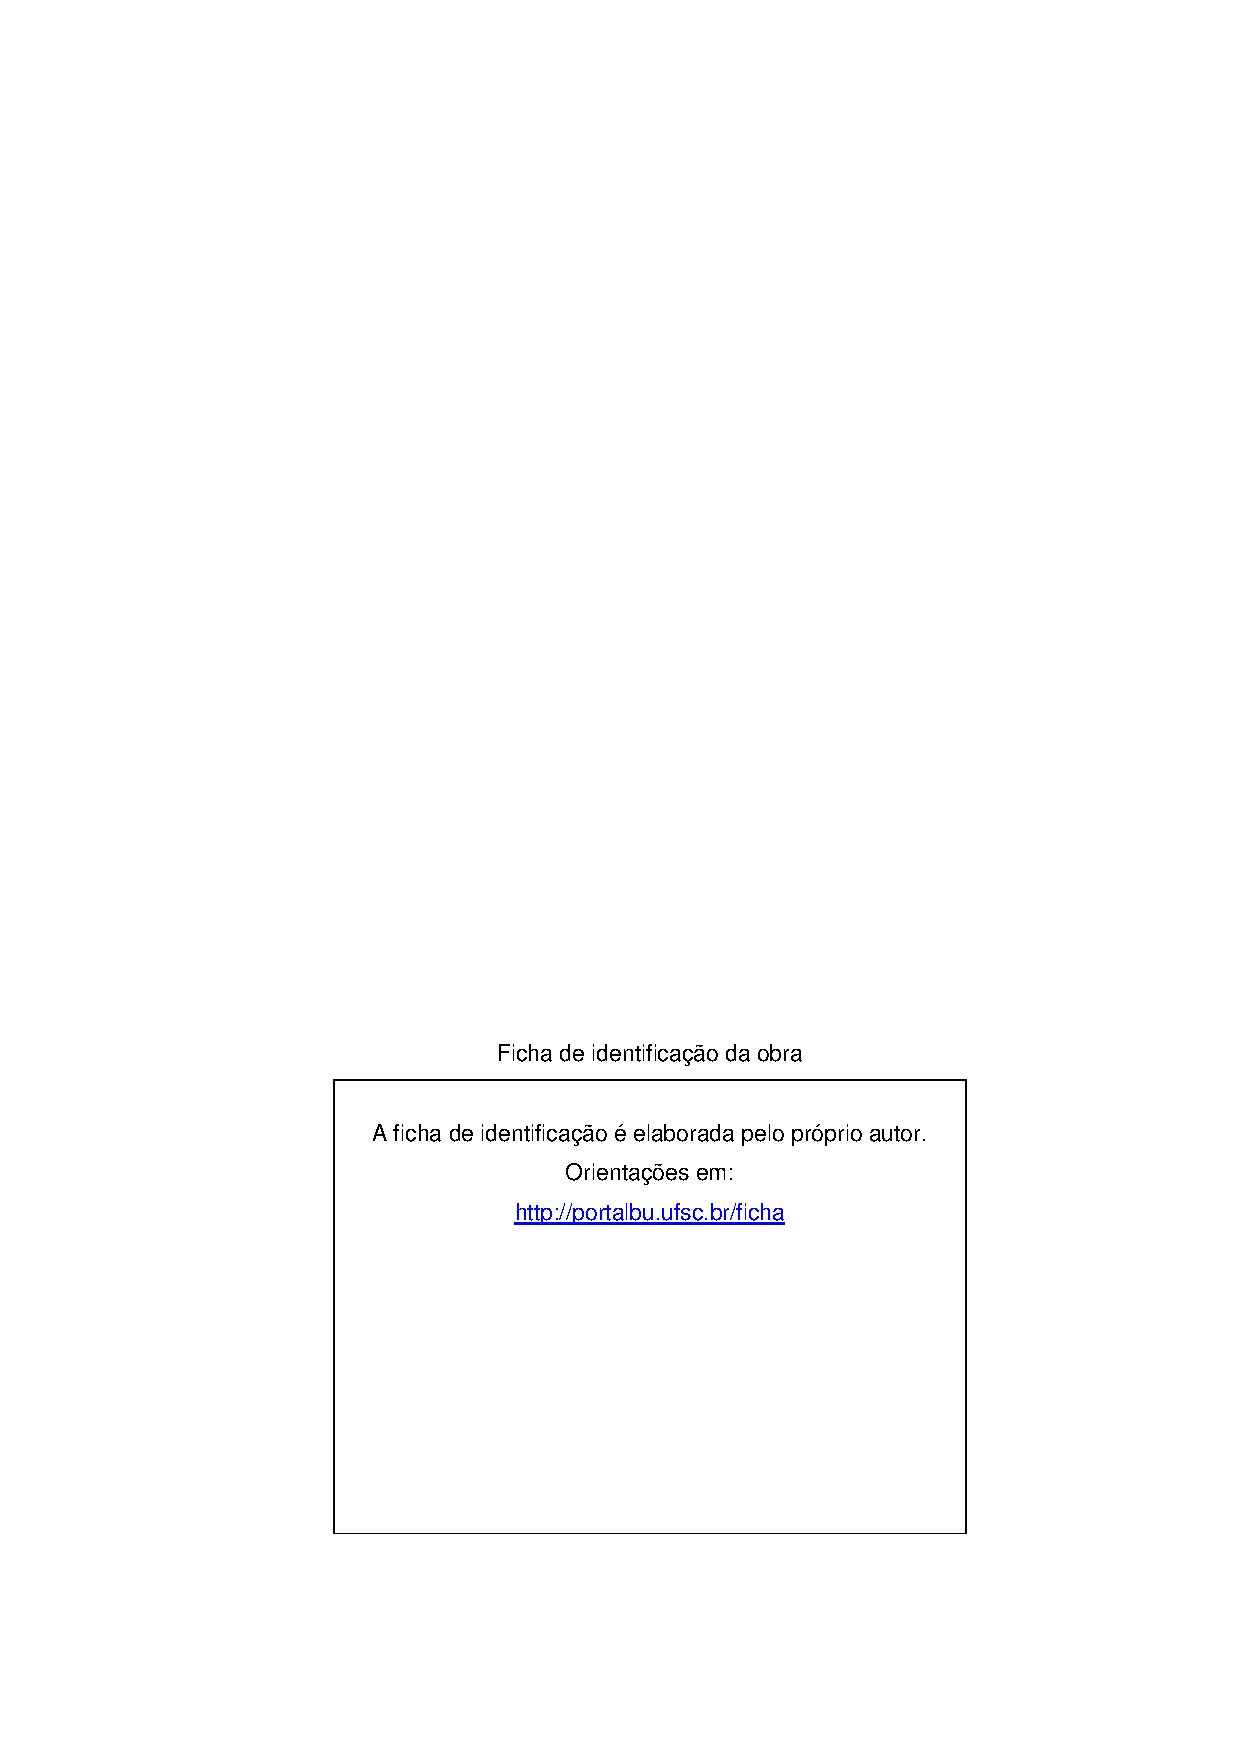
\includepdf{pictures/Ficha_Catalografica.pdf}
    \ifforcedinclude\else\cleardoublepage\fi
\fi


% Inserir errata

% Inserir folha de aprovação. Isto é um exemplo de Folha de aprovação, elemento obrigatório da
% NBR 14724/2011 (seção 4.2.1.3). Você pode utilizar este modelo até a aprovação do trabalho.
% Após isso, substitua todo o conteúdo deste arquivo por uma imagem da página assinada pela
% banca com o comando abaixo:
\ifforcedinclude\else\cleardoublepage\fi


\addtotextpreliminarycontent{\lang{Approval Sheet}{Folha de Aprovação}}

\begin{folhadeaprovacao}

    \begin{center}
        {\imprimirautor}

        \begin{center}
            \ABNTEXchapterfont\bfseries\MakeUppercase{\imprimirtitulo}\ifnotempty{\imprimirsubtitulo}{: \imprimirsubtitulo}
        \end{center}

        \begin{minipage}{\textwidth}
            \lang
            {
                This \imprimirtipotrabalho~was considered appropriate to get the \imprimirformacao,
                \ifnotempty{\imprimirarea}{in the area of \imprimirarea,}
                and it was approved by the \imprimirprograma~of \imprimircentro~of \imprimirinstituicao.
            }
            {
                Este(a) \imprimirtipotrabalho~foi julgado adequado(a) para obtenção do Título de \imprimirformacao,
                \ifnotempty{\imprimirarea}{na área de concentração de \imprimirarea,}
                e foi aprovado em sua forma final pelo \imprimirprograma~
                do \imprimircentro~da \imprimirinstituicao.
            }
         \end{minipage}%
    \end{center}

    \begin{center}
        \imprimirlocal, \imprimirdata.
    \end{center}

    \assinatura{%
        \textbf{\imprimircoordenador} \\
        \imprimircoordenadorRotulo~\lang{of}{do} \imprimirprograma
    }

    % \newpage
    \begin{flushleft}
        \textbf{\lang{Examination Board}{Banca Examinadora}:}
    \end{flushleft}

    \assinatura{%
        \textbf{\imprimirorientador} \\ \imprimirorientadorRotulo\\
        \imprimirinstituicao~--~\imprimirinstituicaosigla
    }

    \ifnotempty{\imprimircoorientador}{%
        \assinatura{%
            \textbf{\imprimircoorientador} \\ \imprimircoorientadorRotulo \\
            \imprimirinstituicao~--~\imprimirinstituicaosigla
        }
    }

    \assinatura{%
        \textbf{Prof. Convidado 1, \lang{PhD.}{Dr.}} \\
        Instituição 1 -- Sigla 1
    }

    \assinatura{%
        \textbf{Prof. Convidado 2, \lang{PhD.}{Dr.}} \\
        Instituição 2 -- Sigla 2
    }

    \assinatura{%
        \textbf{Prof. Convidado 3, \lang{PhD.}{Dr.}} \\
        Instituição 3 -- Sigla 3
    }

    \assinatura{%
        \textbf{Prof. Convidado 4, \lang{PhD.}{Dr.}} \\
        Instituição 4 -- Sigla 4
    }

\end{folhadeaprovacao}


% \includepdf{pictures/folhadeaprovacao_final.pdf}


% Dedicatória
%\ifforcedinclude\else\cleardoublepage\fi
%\ifforcedinclude\else

\addtotextpreliminarycontent{\lang{Dedicatory}{Dedicatória}}

\begin{dedicatoria}

    \vspace*{\fill}
    \centering
    \noindent
    \textit{\lang
    {
        This work is dedicated to adult children who, \\
        When small, dreamed of becoming scientists.
    }
    {
        Este trabalho é dedicado às crianças adultas que,\\
        quando pequenas, sonharam em se tornar cientistas.
    }}
    \vspace*{\fill}

\end{dedicatoria}


\fi

% Agradecimentos
\ifforcedinclude\else\cleardoublepage\fi


\addtotextpreliminarycontent{\lang{Acknowledgement}{Agradecimentos}}

\begin{agradecimentos}

\lang
{
    Greetings.
}
{

    Os meus agradecimentos são direcionados aos meus professores orientadores, o professor Andrea Piga Carboni que me nestes
    últimos 3 anos me acompanhou e orientou com extrema atenção desde o planejamento do trabalho até sua conclusão,
    e ao meu co-orientador, e o professor Marcos Alves Rabelo, pela excelente orientação sempre que necessário, principalmente
    nas etapas experimentais do trabalho.

}

\end{agradecimentos}


%Mesmo padrão da seção primária, porém sem indicativo numérico. Assim como: Dedicatória, Resumo, Abstract, Sumário, Listas, Referências, Apêndices e Anexos.
%
%
%Corpo do texto, fonte 10,5, justificado, recuo especial da primeira linha de 1 cm, espaçamento simples.
%


% Epígrafe
%\ifforcedinclude\else\cleardoublepage\fi
%

\addtotextpreliminarycontent{\lang{Epigraph}{Epigrafe}}

\begin{epigrafe}

\vspace*{\fill}\lang
{
    \begin{flushright}
        \textit{``Learn from yesterday, live for today, hope for tomorrow. The important thing is not to stop questioning.''} \\ Albert Einstein
    \end{flushright}
    \begin{flushright}
        \textit{``The true sign of intelligence is not knowledge but imagination.''} \\  Albert Einstein
    \end{flushright}
    \begin{flushright}
        \textit{``Peace cannot be kept by force; it can only be achieved by understanding.''} \\ Albert Einstein
    \end{flushright}
    \begin{flushright}
        \textit{``Whoever is careless with the truth in small matters cannot be trusted with important matters.''} \\ Albert Einstein
    \end{flushright}
    \begin{flushright}
        \textit{``Extraordinary claims require extraordinary evidence''} \\ Carl Sagan
    \end{flushright}
    \begin{flushright}
        \textit{``Catholic, which I was until I reached the age of reason.''} \\ George Carlin
    \end{flushright}
    \begin{flushright}
        \textit{``We made too many wrong mistakes.''} \\ Yogi Berra
    \end{flushright}
}
{
    \begin{flushright}
        \textit{``Assim como aquele pecado da juventude, este documento te perseguirá pelo resto da vida.''} \\ Enio Valmor Kassick
    \end{flushright}
    \begin{flushright}
        \textit{``Estupidez trará mais autoconfiança do que o conhecimento e a bravura juntas. \englishword{\showfont}''} \\ Adriano Ruseler
    \end{flushright}
}

\end{epigrafe}





% Ajusta o espaçamento dos parágrafos do resumo
\setlength{\absparsep}{18pt}

% RESUMOS
\ifforcedinclude\else\cleardoublepage\fi


\newcommand{\imprimirbrazilabstract}{%
    \cleardoublepage\phantomsection
    \addtotextpreliminarycontent{Resumo em Português}
    \begin{otherlanguage*}{brazil}
    \begin{resumo}[Resumo]

        Segundo a \textcite[3.1-3.2]{NBR6028:2003}, o resumo deve ressaltar o
        objetivo, o método, os resultados e as conclusões do documento. A ordem e a extensão
        destes itens dependem do tipo de resumo (informativo ou indicativo) e do
        tratamento que cada item recebe no documento original. O resumo deve ser
        precedido da referência do documento, com exceção do resumo inserido no
        próprio documento. (\ldots) As palavras-chave devem figurar logo abaixo do
        resumo, antecedidas da expressão Palavras-chave:, separadas entre si por
        ponto e finalizadas também por ponto.

        Além disso, na UFSC o texto do resumo deve ser digitado, em um único bloco, sem espaço de parágrafo. O resumo deve
        ser significativo, composto de uma sequência de frases concisas, afirmativas e não de uma
        enumeração de tópicos. Não deve conter citações. Deve usar o verbo na voz passiva. Abaixo do
        resumo, deve-se informar as palavras-chave (palavras ou expressões significativas retiradas do
        texto) ou, termos retirados de thesaurus da área. \englishword{\showfont}

        \imprimirpalavraschave{Palavras-chaves}{\begin{inparaitem}[]\palavraschaveportugues\end{inparaitem}}

    \end{resumo}
    \end{otherlanguage*}
}


\newcommand{\imprimirenglishabstract}{%
    % https://tex.stackexchange.com/questions/20987/changing-babel-package-inside-a-single-chapter
    % https://tex.stackexchange.com/questions/36526/multiple-language-document-babel-selectlanguage-vs-begin-endotherlanguage
    \cleardoublepage\phantomsection
    \addtotextpreliminarycontent{English's Abstract}
    \begin{otherlanguage*}{english}
    \begin{resumo}[Abstract]

        This is the English abstract.

        \imprimirpalavraschave{Keywords}{\begin{inparaitem}[]\palavraschaveingles\end{inparaitem}}

    \end{resumo}
    \end{otherlanguage*}
}


% \newcommand{\imprimirfrenchabstract}{%
%     \addtotextpreliminarycontent{Français Résumé}
%     \begin{resumo}[Résumé]
%       \begin{otherlanguage*}{french}
%           Il s'agit d'un résumé en français.

%           \imprimirpalavraschave{Mots-clés}{latex. abntex. publication de textes.}
%       \end{otherlanguage*}
%     \end{resumo}
% }


% \newcommand{\imprimirspanishabstract}{%
%     \addtotextpreliminarycontent{Español Resumen}
%     \begin{resumo}[Resumen]
%       \begin{otherlanguage*}{spanish}
%           Este es el resumen en español.

%           \imprimirpalavraschave{Palabras clave}{latex. abntex. publicación de textos.}
%       \end{otherlanguage*}
%     \end{resumo}
% }


\makeatletter
\ifenglish
    \@ifundefined{imprimirbrazilabstract}{}{\imprimirbrazilabstract}

    % https://tex.stackexchange.com/questions/331108/times-new-roman-in-latex-just-some-text
    % https://tex.stackexchange.com/questions/11707/how-to-force-output-to-a-left-or-right-page
    % https://tex.stackexchange.com/questions/132966/do-not-display-chapter-title-in-memoir-class
    \cleardoublepage\phantomsection
    \pretextualchapter{Resumo Expandido}
    \addtotextpreliminarycontent{Resumo Expandido}

    \begin{otherlanguage*}{brazil}
        \setlength{\parskip}{0.2cm}
        \setlength{\parindent}{0.0cm}
        \fontfamily{ptm}\selectfont

        \section*{Introdução}
        O resumo expandido é previsto na Resolução Normativa nº 95/CUn/2017, Art. 55, § 2, de 4 de
        abril de 2017, e exigido para teses e dissertações escritas em idiomas estrangeiros (com
        exceção dos cursos pertinentes ao estudo de idiomas estrangeiros – Programa de Pós-Graduação
        em Estudos da Tradução e Programa de Pós-Graduação em Inglês: Estudos Linguísticos e
        Literários).

        O resumo expandido é considerado um elemento pré-textual e deverá ser incluído no trabalho
        após o resumo e antes do abstract. Deverá iniciar em página impar (no anverso de uma folha)
        continuando no verso da folha. O texto deverá seguir o formato A5, com margens espelhadas:
        superior 2,0 cm, inferior 1,5 cm, interna 2,5 cm e externa 1,5. Deve ser empregada a fonte
        Time New Roman.  Todo o texto deve ser digitado em tamanho 10,5. O espaçamento entre as
        linhas deverá ser simples. A expressão “resumo expandido” deve seguir a mesma tipografia das
        demais sessões primárias do trabalho.

        O texto do resumo expandido deve ser redigido em português e conter as seguintes seções (ver
        modelo): Introdução, Objetivos, Metodologia, Resultados e Discussão e Considerações Finais.
        Deve apresentar no mínimo duas (02) e, no máximo, cinco (05) páginas contendo a mesma
        formatação em A5 do resumo e do abstract, bem como palavras-chave. \englishword{\showfont}

        \section*{Objetivos}
        Lorem ipsum dolor sit amet, consectetur adipiscing elit. Phasellus vitae dolor lacus. Ut
        accumsan vitae felis nec porttitor. Integer interdum fringilla feugiat. Nullam pulvinar sit
        amet tellus eget maximus. Donec sit amet magna eget justo semper fermentum vel eget velit.
        In iaculis imperdiet mauris, ac ornare libero placerat non. Nulla libero lectus, ullamcorper
        ac ornare eget, pulvinar ac nulla. Curabitur vestibulum non nisl eget sagittis. Proin
        gravida lacus id eros bibendum interdum. Mauris ullamcorper elementum tortor sed consequat.
        Integer tempus, est a lobortis vehicula, nisi mi fringilla augue, non semper leo metus in
        quam. Etiam in leo maximus, pulvinar mi eget, vehicula risus. Donec sed dui semper, dictum
        eros at, suscipit felis.

        Nam sagittis vel orci at tempus. Nulla non pellentesque eros.
        Quisque cursus leo massa, eu ultricies nisl lacinia a. Nulla sit amet elementum ligula.
        Proin sodales venenatis dictum. Ut et est cursus, vulputate velit et, viverra odio. Interdum
        et malesuada fames ac ante ipsum primis in faucibus. Maecenas purus diam, tempor a semper
        et, finibus a ex. Cras sagittis felis urna, et consequat arcu lacinia ut. Praesent blandit
        venenatis ante nec porta. Duis rutrum, tellus vitae ullamcorper auctor, lectus ex laoreet
        est, ac tristique ipsum arcu vitae nibh. Nam efficitur felis ut mi consectetur, nec auctor
        odio ornare. In tempor vulputate urna, vitae cursus enim egestas eu. Proin diam augue,
        dignissim vitae ligula eget, lobortis ornare odio. Duis quis elit augue. Fusce quis rhoncus
        tortor. Donec hendrerit at massa a mattis. Sed ipsum neque, aliquam ut sem sed, ultrices
        varius ligula. Suspendisse blandit, dolor ac rhoncus lacinia, dolor purus cursus purus, et
        accumsan orci neque a leo.

        \section*{Metodologia}
        Quisque efficitur dolor in lectus dapibus elementum. Nam ultrices blandit consectetur.
        Nullam ultricies sit amet odio quis placerat. Aenean eget est elit. Maecenas et nulla dolor.
        Orci varius natoque penatibus et magnis dis parturient montes, nascetur ridiculus mus. In
        pulvinar velit sed mi sagittis ornare. Aenean rutrum suscipit egestas. Phasellus pharetra
        eget ex in volutpat. Quisque eu arcu nunc. Vivamus arcu ligula, pharetra at rhoncus sit
        amet, pulvinar sed eros. Sed porta ipsum ipsum, et fermentum magna volutpat sed. Vivamus
        pharetra facilisis orci, sit amet luctus nisl pretium id. Sed consequat, arcu et congue
        pulvinar, risus enim aliquet purus, eget venenatis libero leo sit amet metus. Maecenas vitae
        elit sapien. Fusce mollis libero et gravida placerat. Proin ut quam quis justo aliquam
        dictum. Donec volutpat convallis suscipit. Vivamus metus nisl, placerat ac enim vitae,
        tempus ultricies odio.

        Aliquam ac vehicula arcu, non bibendum nulla. Morbi libero sem,
        imperdiet vel quam et, posuere tempus nunc. Maecenas dictum magna sit amet ligula facilisis
        commodo. Aliquam tellus diam, ornare vel elementum in, dignissim id purus. Ut at tortor non
        sem molestie euismod non at turpis. Phasellus vitae bibendum tellus. Suspendisse odio enim,
        faucibus eget congue quis, semper sit amet tortor. Sed ac lectus est. Pellentesque nec
        mattis mi, et varius dolor. Aliquam quis massa ac tellus malesuada sollicitudin. Maecenas
        ultrices risus massa, nec auctor risus sagittis id. Praesent a sapien nulla. Donec
        tincidunt, metus quis hendrerit facilisis, enim augue convallis elit, sed consequat lacus
        odio vitae magna.

        \section*{Resultados e Discussão}
        Nullam sed cursus leo. Donec commodo volutpat hendrerit. Fusce et tempus lectus, feugiat
        consequat est. Class aptent taciti sociosqu ad litora torquent per conubia nostra, per
        inceptos himenaeos. Nam quis cursus mauris, non tempus orci. Phasellus lobortis et mauris at
        vulputate. Sed nec nisl elementum lorem commodo gravida non a enim. Phasellus neque erat,
        aliquet ac ligula ac, maximus vestibulum sem. Vestibulum vel tincidunt turpis. Donec lacinia
        rutrum dolor dapibus bibendum. Mauris pharetra nibh nec tincidunt iaculis. Vivamus pharetra
        bibendum nisl eget blandit. In lobortis diam non justo eleifend, id lobortis ante fringilla.
        Donec libero tortor, suscipit vestibulum vestibulum id, rutrum accumsan turpis. Phasellus
        sollicitudin luctus tincidunt. Suspendisse potenti. Nam semper metus et mi pharetra, in
        pretium ligula fermentum. Integer consectetur, orci non placerat feugiat, dui ex gravida
        augue, vel placerat ligula augue vel velit. Aliquam sollicitudin pellentesque congue. Donec
        vitae turpis in ante posuere posuere. Pellentesque eu justo leo. Donec quis elit vitae leo
        varius luctus quis eget justo.

        Vestibulum elementum ex neque, quis commodo tortor porttitor
        mattis. Mauris vel sagittis turpis. Aenean ligula turpis, eleifend at felis sed, cursus
        condimentum orci. Fusce accumsan est odio, eu venenatis massa sodales in. Curabitur a tempor
        nisl. Quisque consequat sed arcu a congue. In viverra, ex ut hendrerit condimentum, urna sem
        euismod eros, nec suscipit turpis dolor eget augue. Aenean posuere tellus et consectetur
        condimentum. Mauris et massa et nulla fringilla interdum. Duis quis posuere elit. Donec at
        ex non arcu faucibus rutrum et vel lectus. Vivamus pellentesque vestibulum rutrum. Sed
        pretium, purus sed efficitur feugiat, nisi justo eleifend nibh, id suscipit nunc massa nec
        lectus. In euismod enim eu sapien dictum sodales. Fusce sit amet vulputate orci. Nulla
        rutrum mauris at purus aliquet, ac sollicitudin leo laoreet. Etiam elementum posuere
        feugiat. Maecenas sed libero non augue fermentum ultricies eget at mi. Aenean auctor
        bibendum lacus, dignissim aliquet est tempus eget. Maecenas tempus, nulla id rhoncus
        suscipit, augue leo auctor mi, eget tincidunt magna mi quis dui. Maecenas ut elit in turpis
        tincidunt ultrices. Nulla id nulla aliquet, porttitor eros quis, egestas justo. Nunc nisi
        quam, egestas a accumsan fermentum, ultricies ac elit.

        Nulla porta auctor vestibulum. Sed
        consectetur lacus molestie iaculis ullamcorper. Proin porta posuere massa a lacinia. Nunc a
        lacinia orci, non vehicula ante. Vestibulum ipsum velit, congue et neque aliquam, imperdiet
        ornare augue. Donec et congue sapien. Pellentesque consequat consectetur neque ut varius. In
        aliquam ex quis ante venenatis dapibus. Vivamus et imperdiet urna. Vestibulum quis nibh
        magna. In a congue lectus, eu sodales nunc. Suspendisse id.

        \section*{Considerações Finais}
        Lorem ipsum dolor sit amet, consectetur adipiscing elit. Phasellus vitae dolor lacus. Ut
        accumsan vitae felis nec porttitor. Integer interdum fringilla feugiat. Nullam pulvinar sit
        amet tellus eget maximus. Donec sit amet magna eget justo semper fermentum vel eget velit.
        In iaculis imperdiet mauris, ac ornare libero placerat non. Nulla libero lectus, ullamcorper
        ac ornare eget, pulvinar ac nulla. Curabitur vestibulum non nisl eget sagittis. Proin
        gravida lacus id eros bibendum interdum. Mauris ullamcorper elementum tortor sed consequat.
        Integer tempus, est a lobortis vehicula, nisi mi fringilla augue, non semper leo metus in
        quam. Etiam in leo maximus, pulvinar mi eget, vehicula risus. Donec sed dui semper, dictum
        eros at, suscipit felis.

        Nam sagittis vel orci at tempus. Nulla non pellentesque eros.
        Quisque cursus leo massa, eu ultricies nisl lacinia a. Nulla sit amet elementum ligula.
        Proin sodales venenatis dictum. Ut et est cursus, vulputate velit et, viverra odio. Interdum
        et malesuada fames ac ante ipsum primis in faucibus. Maecenas purus diam, tempor a semper
        et, finibus a ex. Cras sagittis felis urna, et consequat arcu lacinia ut. Praesent blandit
        venenatis ante nec porta. Duis rutrum, tellus vitae ullamcorper auctor, lectus ex laoreet
        est, ac tristique ipsum arcu vitae nibh. Nam efficitur felis ut mi consectetur, nec auctor
        odio ornare. In tempor vulputate urna, vitae cursus enim egestas eu. Proin diam augue,
        dignissim vitae ligula eget, lobortis ornare odio. Duis quis elit augue. Fusce quis rhoncus
        tortor. Donec hendrerit at massa a mattis. Sed ipsum neque, aliquam ut sem sed, ultrices
        varius ligula. Suspendisse blandit, dolor ac rhoncus lacinia, dolor purus cursus purus, et
        accumsan orci neque a leo.


        \imprimirpalavraschave{Palavras-chaves}{\begin{inparaitem}[]\palavraschaveportugues\end{inparaitem}}

    \end{otherlanguage*}

    \@ifundefined{imprimirenglishabstract}{}{\imprimirenglishabstract}

\else
    \@ifundefined{imprimirbrazilabstract}{}{\imprimirbrazilabstract}
    \@ifundefined{imprimirenglishabstract}{}{\imprimirenglishabstract}
\fi

\@ifundefined{imprimirfrenchabstract}{}{\imprimirfrenchabstract}
\@ifundefined{imprimirspanishabstract}{}{\imprimirspanishabstract}
\makeatother



% Some tables of contents
\ifforcedinclude\else
{
    % https://tex.stackexchange.com/questions/179506/disable-colorlinks-locally-or-just-for-the-toc
    \hypersetup{hidelinks}

    % inserir lista de figuras
    \ifforcedinclude\else\cleardoublepage\fi
    % https://tex.stackexchange.com/questions/234398/list-of-figures-and-tables-when-there-are-no-figures-or-tables
    \whenlistisnotempty{\listfigurename}{%
        \addtotextpreliminarycontent{\listfigurename}
        % https://tex.stackexchange.com/questions/121879/remove-spacing-between-per-chapter-figures-in-lof
        {\renewcommand{\addvspace}[1]{}
        \listoffigures*}
    }{\pdfbookmark[0]{\listfigurename}{lof}}

    % inserir lista de quadros
    \ifforcedinclude\else\cleardoublepage\fi
    % https://tex.stackexchange.com/questions/234398/list-of-figures-and-tables-when-there-are-no-figures-or-tables
    \whenlistisnotempty{\listofquadrosname}{%
        \addtotextpreliminarycontent{\listofquadrosname}
        % https://tex.stackexchange.com/questions/121879/remove-spacing-between-per-chapter-figures-in-lof
        {\renewcommand{\addvspace}[1]{}
        \listofquadros*}
    }{\pdfbookmark[0]{\listofquadrosname}{loq}}

    % inserir lista de tabelas
    \ifforcedinclude\else\cleardoublepage\fi
    % https://tex.stackexchange.com/questions/234398/list-of-figures-and-tables-when-there-are-no-figures-or-tables
    \whenlistisnotempty{\listtablename}{%
        \addtotextpreliminarycontent{\listtablename}
        % https://tex.stackexchange.com/questions/121879/remove-spacing-between-per-chapter-figures-in-lof
        {\renewcommand{\addvspace}[1]{}
        \listoftables*}
    }{\pdfbookmark[0]{\listtablename}{lot}}

    % inserir códigos fonte (List of Listings `lol`)
    % https://tex.stackexchange.com/questions/511519/latex-keeps-showing-minted-environment-as-figures-instead-of-listening/511579#511579
    \ifforcedinclude\else\cleardoublepage\fi
    % https://tex.stackexchange.com/questions/234398/list-of-figures-and-tables-when-there-are-no-figures-or-tables
    \whenlistisnotempty{\lstlistlistingname}{%
        \addtotextpreliminarycontent{\lstlistlistingname}
        % https://tex.stackexchange.com/questions/121879/remove-spacing-between-per-chapter-figures-in-lof
        {\renewcommand{\addvspace}[1]{}
        \lstlistoflistings*}
    }{\pdfbookmark[0]{\lstlistlistingname}{lol}}
}
\fi


% inserir lista de abreviaturas e siglas
\ifforcedinclude\else\cleardoublepage\fi


%\addtotextpreliminarycontent{\lang{List of Acronyms}{Lista de Siglas}}
%
%\begin{siglas}
%    \item[ABNT] \lang{Brazilian Association of Technical Standards}{Associação Brasileira de Normas Técnicas}
%    \item[abnTeX] \lang{Absurd Standards for TeX}{ABsurdas Normas para TeX}
%\end{siglas}



% Inserir lista de símbolos
\ifforcedinclude\else\cleardoublepage\fi

\addtotextpreliminarycontent{\lang{List of Symbols}{Lista de Símbolos}}

% Devam aparecer na mesma ordem de ocorrência no texto.
\begin{simbolos}

    \item[$ F_{i} $] {Forças resultantes aplicadas no corpo no eixo i}
    \item[$ M_{i} $] {Momentos aplicados no corpo no eixo i}

    \item[$ \varepsilon $] {Deformação presente no material}
    \item[$ l $] {Comprimento do corpo após deformação}
    \item[$ l_0 $] {Comprimento do corpo sem deformação}

    \item[$ \sigma $] {Tensão interna do material}
    \item[$ E $] {Módulo de elasticidade do material}

    \item[$ \delta $] {Variação de comprimento de uma barra sob tração}
    \item[$ P $] {Carga aplicada no corpo}
    \item[$ A $] {Área da seção transversal}
    \item[$ L $] {Comprimento da barra}

%    \item[$ \tau $] {Tensão torcional no material}
%    \item[$ G $] {Módulo de elasticidade torsional do material}
%    \item[$ r $] {Raio da seção transversal circular}
%    \item[$ \theta $] {Ângulo de deformação}
%
%    \item[$ \nu $] {Módulo de poisson do material}
%
%    \item[$ T $] {Torque aplicado no eixo}
%    \item[$ J $] {Momento polar de inércia da seção transversal}

    \item[$ M $] {Momentos fletor na viga}
    \item[$ I $] {Momento de inércia da seção transversal}
    \item[$ y $] {Distância entre limite e o centróide da área da seção transversal}

    \item[$ k $] {Fator de sensiblidade do extensômetro}
    \item[$ R_s $] {Resistência nominal do extensômetro}
    \item[$ \Delta R $] {Variação de resistência no extensômetro causada pela deformação}

    \item[$ V_{out} $] {Tensão de saída da ponte de wheatstone}
    \item[$ V_{out} $] {Tensão de excitação da ponte de wheatstone}
    \item[$ R_i $] {Resistência nominal dos resistores da ponte de wheatstone}

    \item[$ \varepsilon_{i} $] {Valor de deformação no extensômetro i}

    \item[$ Gain(A) $] {Grau de amplificação do amplificador de sinal}
    \item[$ input $] {Sinal de entrada}
    \item[$ output $] {Sinal amplificado}

    \item[$ \overline{x} $] {Valor médio das amostras}
    \item[$ x_i $] {Valor nominal da amostra i}
    \item[$ n $] {Quantidade de amostras}

    \item[$ Dp $] {Desvio Padrão}

    \item[$ \chi^{2} $] {Valor de chi quadrado}
    \item[$ observed_i $] {Valor experimental observado da amostra i}
    \item[$ expected_i $] {Valor experimental esperado da amostra i}

    \item[$ F(W) $] {Função de calibração}
    \item[$ W $] {Valor nominal do sinal}
    \item[$ W_{high} $] {Carga de calibração de massa alta}
    \item[$ W_{low} $] {Carga de calibração de massa baixa}
    \item[$ output_{high} $] {Valor nominal do sinal obtido pela aplicação da carga alta}
    \item[$ output_{low} $] {Valor nominal do sinal obtido pela aplicação da carga baixa}

\end{simbolos}


% How to remove the self-reference of the ToC from the ToC?
% https://tex.stackexchange.com/questions/10943/how-to-remove-the-self-reference-of-the-toc-from-the-toc
\ifforcedinclude\else\cleardoublepage\fi

\begin{KeepFromToc}
    % https://tex.stackexchange.com/questions/35/what-does-overfull-hbox-mean
    % https://tex.stackexchange.com/questions/59122/how-to-avoid-using-sloppy-document-wide-to-fix-overfull-hbox-problems
    % https://tex.stackexchange.com/questions/257007/adding-color-to-table-of-contents-and-section-headings
    {
        % https://tex.stackexchange.com/questions/179506/disable-colorlinks-locally-or-just-for-the-toc
        \hypersetup{hidelinks}

        % https://tex.stackexchange.com/questions/65711/underfull-vbox-badness-10000-with-memoir
        \raggedbottom

        % https://tex.stackexchange.com/questions/49887/overfull-hbox-warning-for-toc-entries-when-using-memoir-documentclass
        % \makeatletter
            % \renewcommand{\@pnumwidth}{2em}
            % \renewcommand{\@tocrmarg}{3em}
        % \makeatother

        % https://tex.stackexchange.com/questions/57544/memoir-mysterious-overfull-hbox-in-toc-when-mathptmx-is-used
        % \setlength{\cftchapternumwidth}{2.25em}

        % Add the table of contents to the brief table of contents
        % https://tex.stackexchange.com/questions/234398/list-of-figures-and-tables-when-there-are-no-figures-or-tables
        \whenlistisnotempty{\contentsname}{%
            \addtotextpreliminarycontent{\contentsname}
            \tableofcontents
        }{\pdfbookmark[0]{\contentsname}{toc}}
    }

\end{KeepFromToc}



    % ELEMENTOS TEXTUAIS
    \textual
    \setlength\beforechapskip{50pt}
    \setlength\midchapskip{20pt}
    \setlength\afterchapskip{20pt}

    % PARTE
    \ifforcedinclude\else\part{\lang{Research}{Pesquisa}}\fi
    \label{primeira_parte}

    % Introdução (exemplo de capítulo sem numeração, mas presente no Sumário)
    
\phantomsection

\chapter{\lang{Introduction}{Introdução}}
\phantomsection

Atualmente, é notado o constante aumento da importância da otimização dos projetos de componentes em projetos de produtos na indústria automotiva, produtos altamente otimizados resultam em um menor custo de material e de fabricação dos componentes, (Hibbeler) afirma que “a carga para a qual um elemento é projetado pode ser diferente das cargas realmente aplicadas. As dimensões estipuladas no projeto de uma estrutura ou máquina podem não ser exatas, na realidade, por causa de erros de fabricação ou cometidos na montagem de seus componentes”.

Segundo (Hibbeler) “Para se garantir a segurança, é preciso escolher uma tensão admissível que restrinja a carga aplicada a um valor menor do que a carga que o elemento pode suportar totalmente.” Então como resposta às incertezas envolvidas no projeto analítico de um componente os projetistas devem projetar componentes que suportam forças superiores às presentes na utilização do componente. O que resulta em altos valores de fator de segurança em um projeto, o que causa impacto monetário e aumento de massa do componente. Uma das maneiras que permite a diminuição de valores de fator de segurança é a alimentação do projeto do componente com dados de cargas que representam o mais próximo o possível aos presentes na situação real.

Dados reais de utilização podem ser obtidos por sensores em componentes reais ou de teste submetidos a situações reais, porém atualmente certos parâmetros não podem ser facilmente medidos de maneira direta em um veículo, dentre eles forças normais e forças torcionais (Nurprasetio 2018). Hibbeler afirma que “as medições de deformação são experimentais e, uma vez obtidas, podem ser relacionadas com as cargas aplicadas, ou tensões, que agem no interior do corpo.” Logo conclui-se que uma maneira direta de medir as forças internas atuantes em um componentes é obtendo os dados de deformação local.

Foi observado que dispositivos utilizados para obter dados de deformação em tempo real com precisão são usualmente utilizados em testes de impacto e de controle de qualidade em componentes pela indústria automotiva, esses dispositivos apresentam altos níveis de precisão e confiabilidade e, consequentemente altos custos, o que inviabiliza sua utilização fora do produto final. Os valores de deformação local em um componente podem ser obtidos utilizando sensores de deformação chamados de extensômetros, esses sensores apresentam uma boa disponibilidade no mercado e são amplamente utilizados em células de carga. Os sinais gerados por esse tipo de sensor devem ser instrumentados, ampliados e convertidos para possibilitar sua obtenção por uma interface controladora.

O presente trabalho propõe o desenvolvimento de um protótipo de um dispositivo de baixo custo para obtenção de dados de deformação em componentes. O desenvolvimento do dispositivo seguirá a metodologia de projeto de produto PRODIP com o objetivo de garantir replicabilidade, permitir futuras otimizações e expansões e facilitar sua implementação em um caso real. Por fim, o funcionamento, efetividade e precisão do protótipo desenvolvido será avaliado comparando dados obtidos pelo protótipo e por um dispositivo industrial homologado, seguindo a metodologia de Stefani (2017).

\section{Objetivos}
% ----------------------------------------------------------

Os objetivos do trabalho são apresentados nas seções a seguir.

% ----------------------------------------------------------
\subsection{Objetivo Geral}
% ----------------------------------------------------------

Desenvolver um dispositivo de baixo custo para obtenção de dados em tempo real de deflexão em componentes mecânicos.


% ----------------------------------------------------------
\subsection{Objetivos Específicos}
% ----------------------------------------------------------

Obter dados de deflexão em vigas

Obter módulo de elasticidade de uma liga desconhecida

Desenvolver utilizando tecnologias de código aberto

Obter valores de precisão do protótipo desenvolvido


% https://tex.stackexchange.com/questions/5076/is-it-possible-to-keep-my-translation-together-with-original-text
% \chapter{\lang{Introduction}{Introdução}}
% \phantomsection

% A Tabela~\ref{tab:a_table_formatacao_de_texto} mostra  informações do modelo de teses da Biblioteca Universitária da UFSC (BU-UFSC).

% % What does [t] and [ht] mean?
% % https://tex.stackexchange.com/questions/8652/what-does-t-and-ht-mean
% %
% % How can I get rid of the LaTeX warning: Float too large for page?
% % https://tex.stackexchange.com/questions/36252/how-can-i-get-rid-of-the-latex-warning-float-too-large-for-page
% %
% % "warning: Text page X contains only floats" How to suppress this warning?
% % https://tex.stackexchange.com/questions/223149/warning-text-page-x-contains-only-floats-how-to-suppress-this-warning
% %
% % Make a table span multiple pages
% % https://tex.stackexchange.com/questions/26462/make-a-table-span-multiple-pages
% %
% % How to make the longtable to work with centering & caption on memoir class?
% % https://tex.stackexchange.com/questions/386541/how-to-make-the-longtable-to-work-with-centering-caption-on-memoir-class
% %
% % How to fix this Package array Error: Only one column-spec allowed?
% % https://tex.stackexchange.com/questions/367069/how-to-fix-this-package-array-error-only-one-column-spec-allowed
% %
% % How to auto adjust my last table column width, and why is there Underfull \vbox badness on this table?
% % https://tex.stackexchange.com/questions/387238/how-to-auto-adjust-my-last-table-column-width-and-why-is-there-underfull-vbox/387251
% \setlength\extrarowheight{2pt}
% \begin{tabularx}{\linewidth}{>{\RaggedRight}p{3cm}|>{\arraybackslash}X}

% \caption[Formatação do texto]{Formatação do texto \showfont}
% \label{tab:a_table_formatacao_de_texto} \\
% \hline
% \endfirsthead

% % How to set font size of footnotes correctly in memoir?
% % https://tex.stackexchange.com/questions/213927/how-to-set-font-size-of-footnotes-correctly-in-memoir
% \multicolumn{2}{p{\dimexpr\textwidth-2\tabcolsep\relax}}{\ufsccaptionsize\tablename~\thetable:
% Formatação do texto (continuação) \showfont} \\
% \hline
% \endhead

% % Set multicolumn width to default table width
% % https://tex.stackexchange.com/questions/99326/set-multicolumn-width-to-default-table-width
% \hline
% \multicolumn{2}{p{\dimexpr\textwidth-2\tabcolsep\relax}}{\footnotesize continua na próxima página\protect\englishword{\showfont}}
% \endfoot

% \hline
% \multicolumn{2}{p{\dimexpr\textwidth-2\tabcolsep\relax}}{\fonte{O autor -- \showfont} }
% \endlastfoot
%     Cor                          & Branco - \englishword{\showfont}                                 \\ \hline
%     Formato do papel             & A4                                                               \\ \hline
%     Gramatura                    & 75                                                               \\ \hline
%     Impressão                    & Frente e verso                                                   \\ \hline
%     Margens                      & Direita e superior 3, Inferior e esquerda: 2.                    \\ \hline
%     Cabeçalho                    & 0,7                                                              \\ \hline
%     Rodapé                       & 0,7                                                              \\ \hline
%     Paginação                    & Externa                                                          \\ \hline
%     Alinhamento vertical         & Superior                                                         \\ \hline
%     Alinhamento do texto         & Justificado                                                      \\ \hline
%     Fonte sugerida               & Times New Roman                                                  \\ \hline
%     Tamanho da fonte             & 12 para o texto incluindo os títulos das seções e subseções.
%                                    As citações com mais de três linhas as legendas das ilustrações
%                                    e tabelas, fonte 10.                                             \\ \hline
%     Espaçamento entre linhas     & Um e meio (1,5)                                                  \\ \hline
%     Espaçamento entre parágrafos & Anterior 0,0; Posterior 0,0                                      \\ \hline
%     Numeração da seção           & As seções  primárias devem  começar  sempre em páginas ímpares.
%                                    Deixar um espaço (simples) entre o título da seção e o texto e
%                                    entre o texto e o título da subseção.                            \\ \hline

% \end{tabularx}


% \begin{figure}
%     \caption{Exemplo de figura}
%     \label{fig:ex01}
%     \centering
%     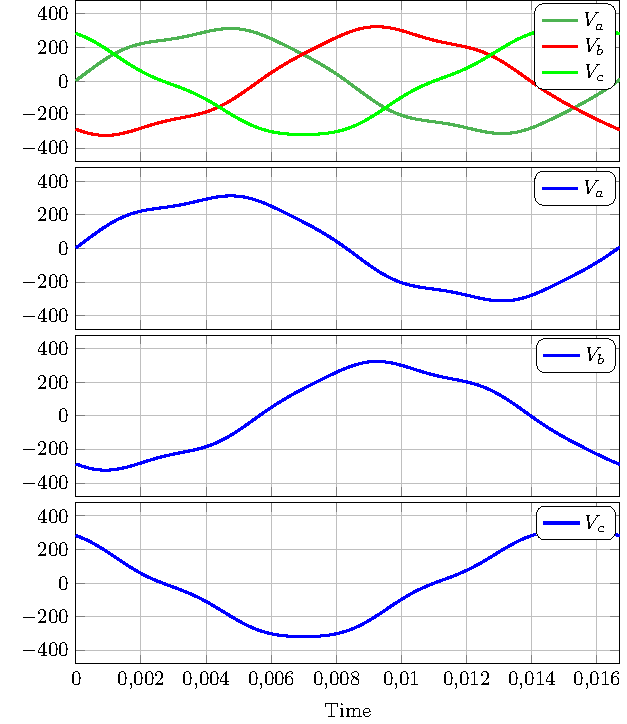
\includegraphics[width=\linewidth]{pictures/ex01}
% \fonte{o autor -- \showfont}
% \end{figure}


% Por exemplo, na \figref{fig:ex01}, tem-se...

% \begin{figure}
%     \caption{Exemplo de aquisição}
%     \label{fig:tek0009}
%     \centering
%     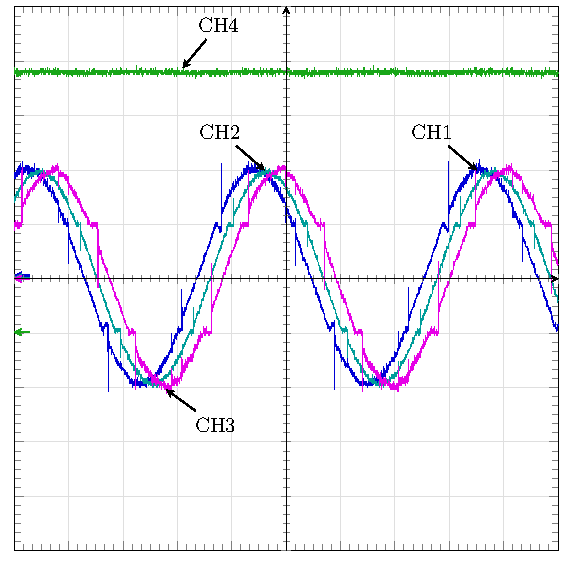
\includegraphics[width=0.9\linewidth]{pictures/tek0009}
%     \fonte{o autor -- \showfont}
% \end{figure}

% Este documento e seu código-fonte são exemplos de referência de uso da classe
% \textsf{abntex2} e do pacote \textsf{abntex2cite}. O documento
% exemplifica a elaboração de trabalho acadêmico (tese, dissertação e outros do
% gênero) produzido conforme a ABNT NBR 14724:2011 \emph{Informação e documentação
% - Trabalhos acadêmicos - Apresentação}.

% A expressão ``Modelo Canônico'' é utilizada para indicar que \abnTeX{} não é
% modelo específico de nenhuma universidade ou instituição, mas que implementa tão
% somente os requisitos das normas da ABNT. Uma lista completa das normas
% observadas pelo \abnTeX{} é apresentada em \textcite{abntex2classe}.

% Sinta-se convidado a participar do projeto \abnTeX{}! Acesse o site do projeto em
% \url{http://abntex2.googlecode.com/}. Também fique livre para conhecer,
% estudar, alterar e redistribuir o trabalho do \abnTeX{}, desde que os arquivos
% modificados tenham seus nomes alterados e que os créditos sejam dados aos
% autores originais, nos termos da ``The \LaTeX{} Project Public
% License''\footnote{\url{http://www.latex-project.org/lppl.txt}}.

% Encorajamos que sejam realizadas customizações específicas deste exemplo para
% universidades e outras instituições --- como capas, folha de aprovação, etc.
% Porém, recomendamos que ao invés de se alterar diretamente os arquivos do
% \abnTeX{}, distribua-se arquivos com as respectivas customizações.
% Isso permite que futuras versões do \abnTeX{}~não se tornem automaticamente
% incompatíveis com as customizações promovidas. Consulte
% \textcite{abntex2-wiki-como-customizar} par mais informações.

% Este documento deve ser utilizado como complemento dos manuais do \abnTeX{}
% \cite{abntex2classe,abntex2cite,abntex2cite-alf} e da classe \textsf{memoir}
% \cite{memoir}.

% Esperamos, sinceramente, que o \abnTeX{} aprimore a qualidade do trabalho que
% você produzirá, de modo que o principal esforço seja concentrado no principal:
% na contribuição científica.

% Equipe \abnTeX{}

% Lauro César Araujo




    % Capitulo com exemplos de comandos inseridos de arquivo externo
    \phantomsection

\chapter{Referencial Teórico}

O presente capítulo apresenta os conceitos teóricos necessários para o desenvolvimento do princípio de funcionamento do dispositivo.
São apresentados tópicos referentes a solicitações mecânicas e resistência dos materiais, princípios de sensoriamento de deformação e instrumentação de extensômetros,
obtenção de sinais e transmissão de dados. Também será apresentado as principais tecnologias necessárias para o processo de desenvolvimento do dispositivo.

\section{SOLICITAÇÕES E RESISTÊNCIA DOS MATERIAIS}

Um entendimento introdutório sobre resistência dos materiais é necessário de modo a entender sobre os comportamentos físicos de um componente mecânico
que sofre a ação de cargas externas. O ponto de partida do estudo da resistência dos materiais é o da análise do comportamento mecânico de um componente em equilíbrio.

Utilizando as equações de estática, deve-se determinar as forças e os momentos resultantes que agem no interior de um corpo, com a finalidade de verificar
e garantir a integridade do mesmo durante o uso \autocite{Hibbeler2010}. Um corpo em equilíbrio, deve satisfazer a \autoref{eq:Eq_110} e \autoref{eq:Eq_120}, que
descrevem o balanço estático conforme a segunda lei de newton.

\begin{equation}\label{eq:Eq_110}%
\mbox{\fontsize{17.28}{21.6}\selectfont\( %
\sum F_{x} = \sum F_{y} = \sum F_{z} = 0
\)} %
\end{equation}

\begin{equation}\label{eq:Eq_120}%
\mbox{\fontsize{17.28}{21.6}\selectfont\( %
\sum M_{x} = \sum M_{y} = \sum M_{z} = 0
\)} %
\end{equation}

onde

$F_{i}$: Forças axiais aplicadas no corpo no eixo "i"

$M_{i}$: Momentos aplicados no corpo no eixo "i"

\hfill

Para ser mantida a condição de integridade do corpo do material sobre forças externas devem estar presentes forças e momentos internos ao seu corpo,
\autocite{Hibbeler2010} ressalta que “Uma das mais importantes aplicações da estática na análise de problemas de resistência dos materiais é poder
determinar a força e o momento resultantes que agem no interior de um corpo e que são necessários para manter a integridade do corpo quando
submetido a cargas externas” e que “a força e o momento que agem em um ponto específico da área secionada de um corpo representam os efeitos resultantes
da distribuição de forças que agem sobre a área secionada”. A \autoref{fig:1010} apresenta uma representação gráfica da atuação de forças internas em um material:

\begin{figure}[htb]
	\caption{\label{fig:1010} Forças internas atuando em um corpo em equilíbrio}
	\begin{center}
		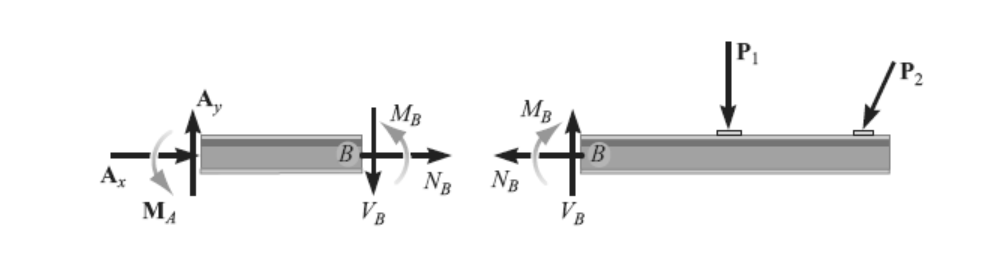
\includegraphics[width=\textwidth]{pictures/1010.png}
	\end{center}
	\fonte{\autocite{Hibbeler2010}}
\end{figure}

Uma vez que se tem a informação das forças internas atuantes em um ponto no corpo e na seção do material, então, pode-se partir para a análise das tensões
e deformações do local de análise.

\subsection{Deformação e limites do material}

Quando um segmento de um corpo sob balanço estático se encontra sob a ação de forças internas, este segmento apresentará uma variação de seu comprimento relativo
à força aplicada. Deformação é definido como a mudança de comprimento por unidade de comprimento, logo, é um valor adimensional,
e é calculada pela \autoref{eq:Eq_130}.\autocite{Norton2011}

\begin{equation}\label{eq:Eq_130}%
\mbox{\fontsize{17.28}{21.6}\selectfont\( %
\varepsilon = \frac{l - l_0}{l_0}
\)} %
\end{equation}

onde

$\varepsilon$: Deformação

$l$: Comprimento da barrra após deformação

$l_0$: Comprimento da barra sem deformação

\hfill

Com o objetivo de descobrir os limites no qual um material pode-se deformar antes de sua ruptura devem ser analisados seus diagramas tensão-deformação.
Hibbeler ressalta a importância na análise desse tipo de diagrama, uma vez que eles proporcionam meios para a obtenção de dados sobre resistência à tração
ou compressão de um material sem independentemente de suas características físicas e geométricas \autocite{Hibbeler2010}. Um exemplo de diagrama tensão-deformação
é mostrado na \autoref{fig:1020}.

\begin{figure}[htb]
	\caption{\label{fig:1020} Exemplo de diagrama tensão-deformação}
	\begin{center}
		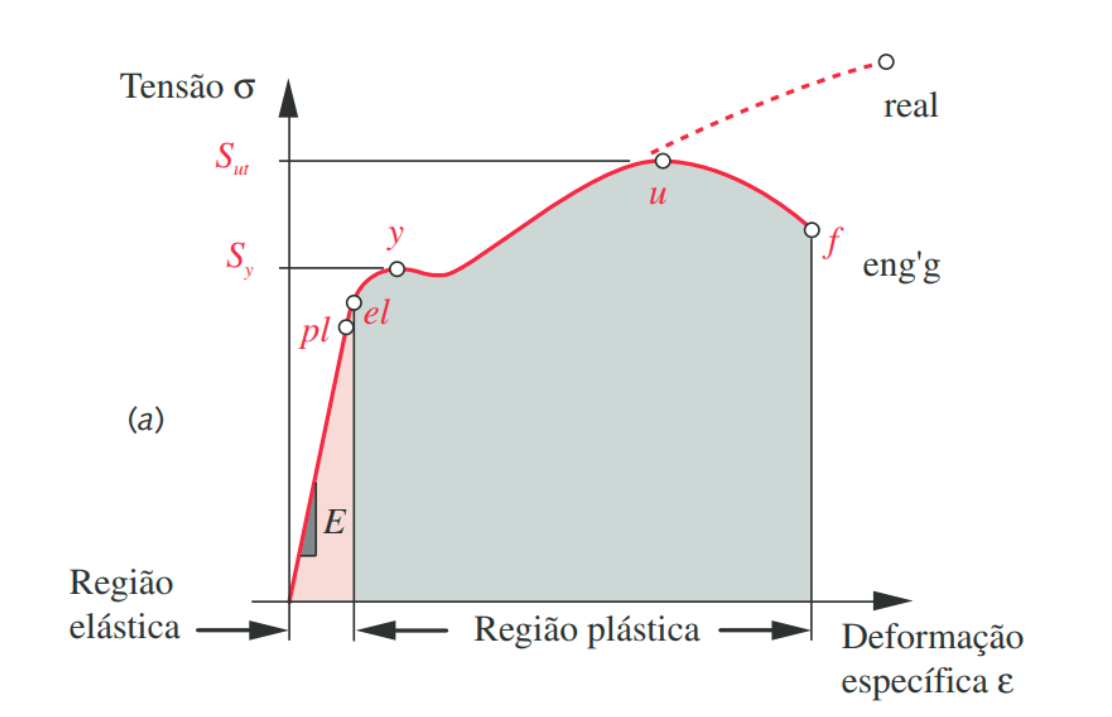
\includegraphics[width=\textwidth]{pictures/1020.png}
	\end{center}
	\fonte{\autocite{Norton2011}}
\end{figure}

Analisando o diagrama anterior pode-se notar uma zona de relacionamento linear entre a força aplicada no corpo de prova utilizado para construir o diagrama e sua
deformação, nesta região é observado o comportamento de deformação elástica do material e sobre seu limite \autocite{Norton2011} afirma que os pontos pl e el
“marca o limiar entre as regiões de comportamento elástico e comportamento plástico do material.
Os pontos $el$ e $pl$ normalmente são tão próximos que eles quase sempre são considerados o mesmo.”

Na maior parte dos materiais de engenharia é verificada uma relação linear entre deformação e tensão dentro da região elástica, logo, um aumento proporcional
na força aplicada em um material resulta em um aumento proporcional das deformações locais caso a condição de tensão esteja dentro do limite elástico, esse fato
foi descoberto por Robert Hooke, em 1676, em molas e é conhecido como Lei de Hooke \autocite{Hibbeler2010}. A lei de Hooke é apresentada na \autoref{eq:Eq_140}.

\begin{equation}\label{eq:Eq_140}%
\mbox{\fontsize{17.28}{21.6}\selectfont\( %
\sigma = E \varepsilon
\)} %
\end{equation}

onde

$\sigma $: Tensão interna do material

$E$: Módulo de elasticidade do material

$\varepsilon$: Deformação presente no material

\hfill

A variável $E$ da equação da Lei de Hooke é representa a inclinação da curva tensão-deformação e é chamada de Módulo de Young, ou módulo de elasticidade do
material \autocite{Norton2011}. Norton também afirma que o Módulo de Young “é uma medida da rigidez do material em sua região elástica e tem as mesmas unidades da tensão.
A maioria dos metais exibe esse comportamento linear e também tem módulos de elasticidade que variam muito pouco com tratamentos térmicos ou com a adição de elementos de liga.”

Para uma barra constituída de um material homogêneo e isotrópico e submetida a forças axiais que tem seu centro de atuação no centro da seção da barra essas cargas
irão gerar uma tensão normal uniforme ao longo do seu comprimento sobre a seção transversal \autocite{Hibbeler2010}.

\begin{figure}[htb]
	\caption{\label{fig:1030} Deflexão de uma barra sob carga de tração}
	\begin{center}
		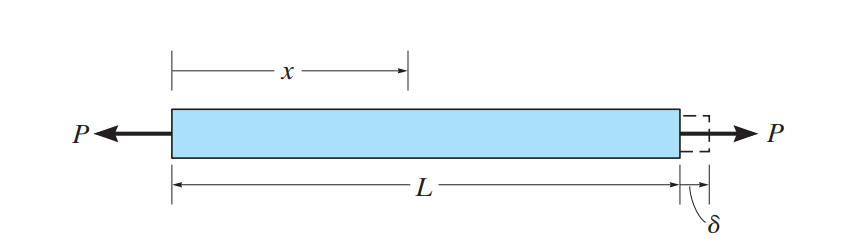
\includegraphics[width=\textwidth]{pictures/1030.png}
	\end{center}
	\fonte{\autocite{Hibbeler2010}}
\end{figure}

O alongamento ou contração de um segmento de reta por unidade de comprimento é denominado deformação normal e segue a \autoref{eq:Eq_150}.

\begin{equation}\label{eq:Eq_150}%
\mbox{\fontsize{17.28}{21.6}\selectfont\( %
\delta = \frac{PL}{AE}
\)} %
\end{equation}

onde

$\delta $: Deformação

$P$: Carga de tração aplicada na barra

$A$: Área da seção transversal

$L$: Comprimento da barra

\hfill

%Para outros tipos de carregamentos também são notados valores de deformação relativos às cargas aplicadas, os principais utilizados no desenvolvimento do experimento são introduzidos não sub subseções abaixo.
%
%\subsection{Deformação de um eixo em torção}
%
%Eixos normalmente são utilizados em situações em que as cargas torcionais são consideráveis, e caso estejam presentes cargas normais ou de flexão em sua utilização, e o material encontra-se em balanço estático, pode-se utilizar as mesmas equações de deformação da análise de barras e vigas. Norton afirma que “quando barras são solicitadas por um momento em relação ao seu eixo longitudinal, diz-se que estão sob torção, esse tipo de momento aplicado é denominado torque e esta situação é comum em eixos que transmitem potência.” A deformação vista no corpo de um eixo sob cargas de torção pura ao longo da sua seção transversal é ilustrada na \autoref{fig:1040}.
%
%\begin{figure}[htb]
%	\caption{\label{fig:1040} Representação do efeito da deflexão em um eixo sob torção}
%	\begin{center}
%		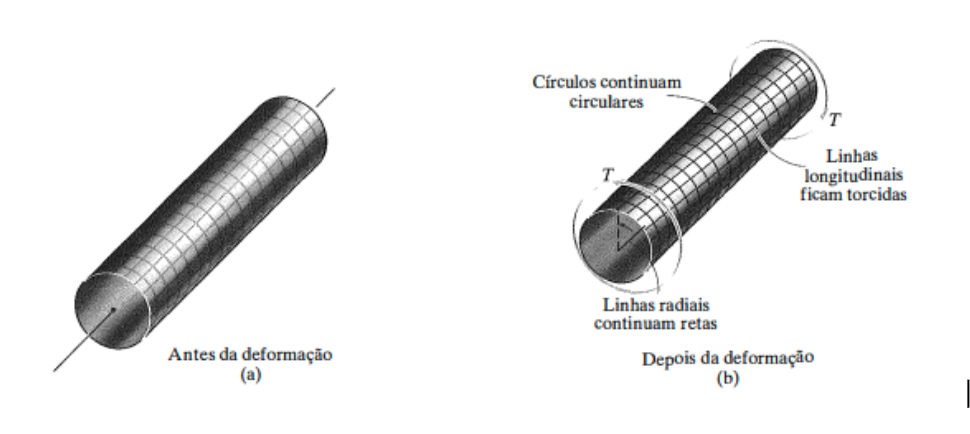
\includegraphics[width=\textwidth]{pictures/1040.png}
%	\end{center}
%	\fonte{\autocite{Hibbeler2010}}
%\end{figure}
%
%A Lei de Hooke para um corpo sob forças de torção é semelhante a mesma para o caso de um corpo em tração ou compressão como apresentada na \autoref{eq:Eq_160}.
%
%\begin{equation}\label{eq:Eq_160}%
%\mbox{\fontsize{17.28}{21.6}\selectfont\( %
%\tau = \frac{Gr\theta}{l_0}
%\)} %
%\end{equation}
%
%onde
%
%$\tau $: Tensão torcional no material
%
%$G$: Módulo de elasticidade torcional
%
%$r$: raio da seção transversal
%
%$\theta$: Ângulo de deformação
%
%$l_0$: Comprimento do material
%
%
%\hfill
%
%Desta vez o módulo presente dessa vez é denominado módulo de elasticidade transversal $G$ que é definido em termos do módulo de elasticidade $E$ e do coeficiente de Poisson $\nu$ do material. O coeficiente de Poisson $\nu$ representa a relação entre a deformação específica lateral e longitudinal do material.\autocite{Norton2011}
%
%\begin{equation}\label{eq:Eq_170}%
%\mbox{\fontsize{17.28}{21.6}\selectfont\( %
%G = \frac{E}{2(1+\nu )}
%\)} %
%\end{equation}
%
%onde
%
%$G$: Módulo de elasticidade torcional
%
%$E$: Módulo de elasticidade do material
%
%$\nu$: Módulo de poisson do material
%
%\hfill
%
%A \autoref{tab:PoissonValues} apresenta os principais valores de coeficiente de poisson para diferentes materiais metálicos. \autocite{Norton2011}
%
%\begin{table}[!ht]
%    \caption{Valores de coeficiente de Poisson para os principais materiais mealicos}
%    \label{tab:PoissonValues}
%    \centering
%    \resizebox{\linewidth}{!}{%
%        \begin{tabular}{ l | c c r } \toprule
%            Material & $\nu$ \\\hline
%            Alumínio & $\SI{0.34}$ \\
%            Cobre & $\SI{0.35}$ \\
%            Ferro 1 & $\SI{0.28}$ \\
%            Aço 2 & $\SI{0.28}$ \\
%            Magnésio 3 & $\SI{0.33}$ \\
%            Titânio 4 & $\SI{0.34}$ \\
%            \bottomrule
%        \end{tabular}}
%\fonte{O autor 2022}
%\end{table}
%
%Assim como visto na \autoref{fig:1040} é notado que a deformação nessa situação não se apresenta como aumento de comprimento do componente, como no caso da uma barra sob cargas axiais, mas por uma distribuição de deslocamentos angulares locais na direção radial da seção do eixo conforme se aumenta a dimensão de comprimento da análise das cargas internas como apresentado na \autoref{fig:1050}.
%
%\begin{figure}[htb]
%	\caption{\label{fig:1050} Deflexão e distribuição de tensão em um eixo sob torção}
%	\begin{center}
%		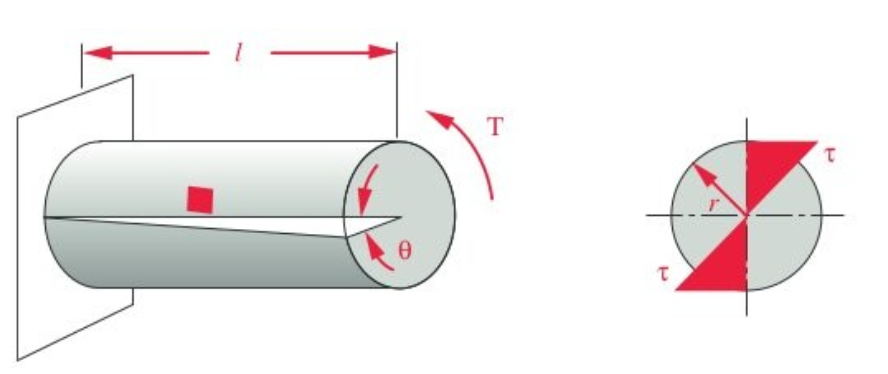
\includegraphics[width=\textwidth]{pictures/1050.png}
%	\end{center}
%	\fonte{\autocite{Norton2011}}
%\end{figure}
%
%A \autoref{eq:Eq_180} é obtida da análise da Lei de Hooke para um eixo em torção.
%
%\begin{equation}\label{eq:Eq_180}%
%\mbox{\fontsize{17.28}{21.6}\selectfont\( %
%\theta = \frac{Tl}{GJ}
%\)} %
%\end{equation}
%
%\hfill
%
%\begin{equation}\label{eq:Eq_190}%
%\mbox{\fontsize{17.28}{21.6}\selectfont\( %
%\tau = \frac{Tr}{J}
%\)} %
%\end{equation}
%
%sendo
%
%$T$: TBD
%
%$r$: TBD
%
%$l$: TBD
%
%$G$: TBD
%
%$J$: TBD
%
%\hfill
%
%Assim como as barras em tração, as equações aqui apresentadas apenas consideram a operação do componente em regime de deformação elástico, logo os valores esperados de θ serão relativamente pequenos para materiais de engenharia.

\subsection{Deformação de uma viga em flexão}

A flexão é presente em um corpo sempre que as forças não são aplicadas na direção normal da sua seção transversal.
Segundo \autocite{Hibbeler2010} “O momento fletor é causado pelas cargas externas que tendem a fletir o corpo em torno de um eixo que se encontra no plano da área.”
e que nesse momento “tende a produzir uma variação linear da deformação normal no interior de uma viga”.
A \autoref{fig:1060} mostra uma representação ilustrativa do efeito do momento fletor em uma viga.

\begin{figure}[htb]
	\caption{\label{fig:1060} Representação do efeito da deflexão em uma viga sob flexão}
	\begin{center}
		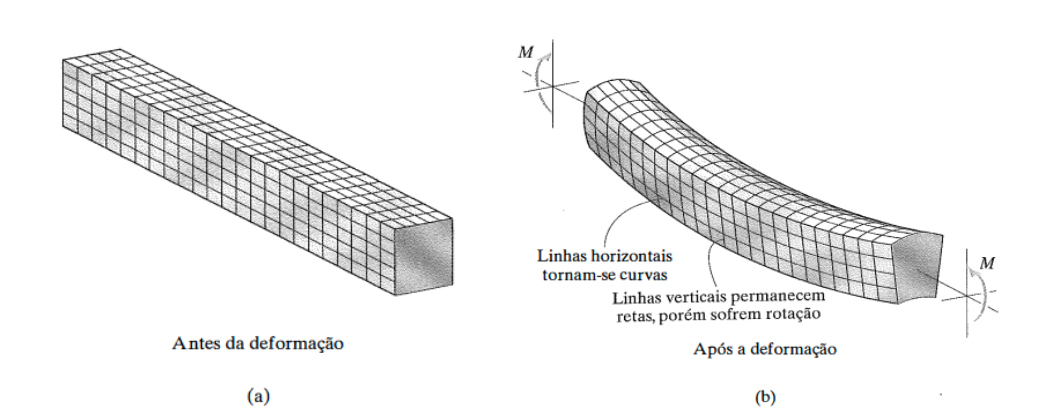
\includegraphics[width=\textwidth]{pictures/1060.png}
	\end{center}
	\fonte{\autocite{Hibbeler2010}}
\end{figure}

Em todo caso em que o material seja homogêneo e isotrópico e que a Lei de Hooke seja aplicável, pode-se relacionar o momento fletor presente com a distribuição de
tensão na seção \autocite{Hibbeler2010}. Deve-se notar que assim como a barra em torção, a tensão, e eventualmente a deflexão presente será função da distância entre o
ponto de interesse e o centro da área da seção transversal do material. A \autoref{eq:Eq_200} caracteriza a distribuição de tensão ao longo da seção do componente.

\begin{figure}[htb]
	\caption{\label{fig:1070} Deflexão e distribuição de tensão em uma sob flexão}10
	\begin{center}
		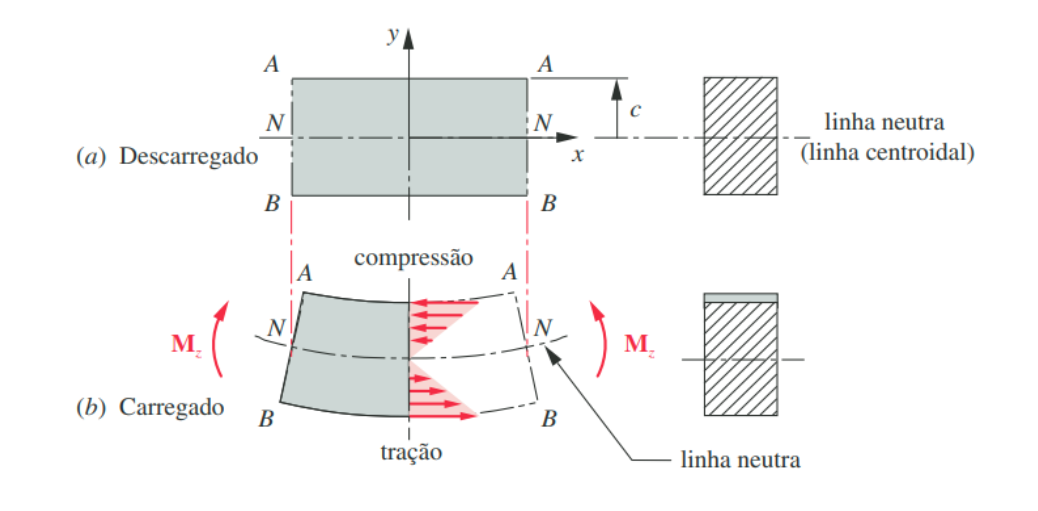
\includegraphics[width=\textwidth]{pictures/1070.png}
	\end{center}
	\fonte{\autocite{Norton2011}}
\end{figure}

\begin{equation}\label{eq:Eq_200}%
\mbox{\fontsize{17.28}{21.6}\selectfont\( %
\sigma = - \frac{My}{I}
\)} %
\end{equation}

onde

$M$: Momento fletor

$y$: Distância entre limite da área e seu centróide

$I$: Momento de inércia da seção transversal

\hfill

O valor de $I$ é igual ao momento de inércia da seção do material sobre carga de flexão e a variável $y$ representa a distância entre o centróide da área e o ponto de
análise de tensão, deve-se notar que as tensões máximas para qualquer corpo em flexão sempre acontecerão na superfície do material, e que enquanto um ponto qualquer
está sob forças de tração, o ponto inverso a este estará sob forças de compressão. Uma vez conhecido o módulo de elasticidade do material e a distribuição de tensão
de na seção de um corpo sob flexão, pode-se obter, utilizando a lei de hooke, os valores de deflexão causados pelas cargas de flexão.

As deformações em um componente podem ser altamente visíveis ou praticamente imperceptíveis se não forem utilizados equipamentos que façam medições precisas
\autocite{Hibbeler2010}. Considerando essa afirmação deve-se também ser estudado o método experimental de obtenção de dados de deflexão nos componentes.

\section{EXTENSOMETRIA}

O extensômetro de resistência elétrica é o dispositivo mais utilizado para medir a deflexão em uma superfície, o princípio de funcionamento desse tipo de sensor é
baseado no efeito de variação de resistência elétrica de um condutor quando ocorre uma variação de área da sua seção transversal \autocite{Hollman2011}.

\begin{figure}[htb]
	\caption{\label{fig:1080} Extensômetro fixado á um corpo de prova}
	\begin{center}
		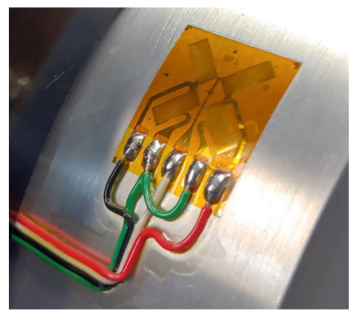
\includegraphics[width=\textwidth]{pictures/1080.png}
	\end{center}
	\fonte{https://binsfeld.com/category/strain-gage/ acesso em fev 2022}
\end{figure}

Caso um extensômetro esteja fortemente fixado a um corpo de um material em uma direção específica, qualquer carga que deforma a superfície desse corpo de prova irá
deformar igualmente o extensômetro, logo pode-se considerar o extensômetro como uma parte integrante do corpo de prova e qualquer deformação que aconteça no corpo de
prova acontecerá igual no extensômetro \autocite{Hibbeler2010}.

O fator de extensão ou gage factor, parâmetro que especifica a relação entre a variação da resistência nominal em um extensômetro para um valor unitário
de deflexão, é um valor especificado pelo fabricante, então, e a resistência nominal do extensômetro são valores especificados pelo fabricante do sensor, então medindo um valor
e variação de resistência elétrica no extensômetro pode-se obter um valor de deformação local \autocite{Hollman2011}. A \autoref{eq:Eq_210} mostra uma relação entre a variação
de resistência elétrica no extensômetro e os parâmetros repassados pelo fabricante.

\begin{equation}\label{eq:Eq_210}%
\mbox{\fontsize{17.28}{21.6}\selectfont\( %
K \varepsilon = \frac{\Delta R_s }{R_s}
\)} %
\end{equation}

sendo

$K$: Gage Factor

$\varepsilon$: Deformação no extensômetro

$\Delta R_s$: Variação de resistência causada pela deformação

$R_s$: Resistência nominal do extensômetro

\hfill

Porém, deve-se notar que os valores de deflexão esperados para um metal dentro de sua zona de deformação elástica são muito pequenos, o que acarreta em pequenas
variações de resistência no extensômetro. Com o objetivo de facilitar a medição da deflexão, devem ser utilizados artifícios de instrumentação como um circuito de ponte
com a finalidade de detectar com maior variação as mudanças de resistência do sensor.

\subsection{Ponte de Wheatstone}

Circuitos de ponte são utilizados para prover melhores medições e precisões em uma variedade de aplicações de medição de resistência elétrica, indutância e capacitância
sob condições tanto estáticas quanto transientes. Dentre diversos tipos de circuitos de ponte a ponte de Wheatstone, demonstrada na \autoref{fig:1090} se
demonstra como um dos tipos de circuito elétrico mais utilizado e facilita a leitura da variação de resistência de sensores que apresentam baixas variações de resistência
elétrica na sua operação. \autocite{Hollman2011}

\begin{figure}[htb]
	\caption{\label{fig:1090} Ponte de Wheatstone}
	\begin{center}
		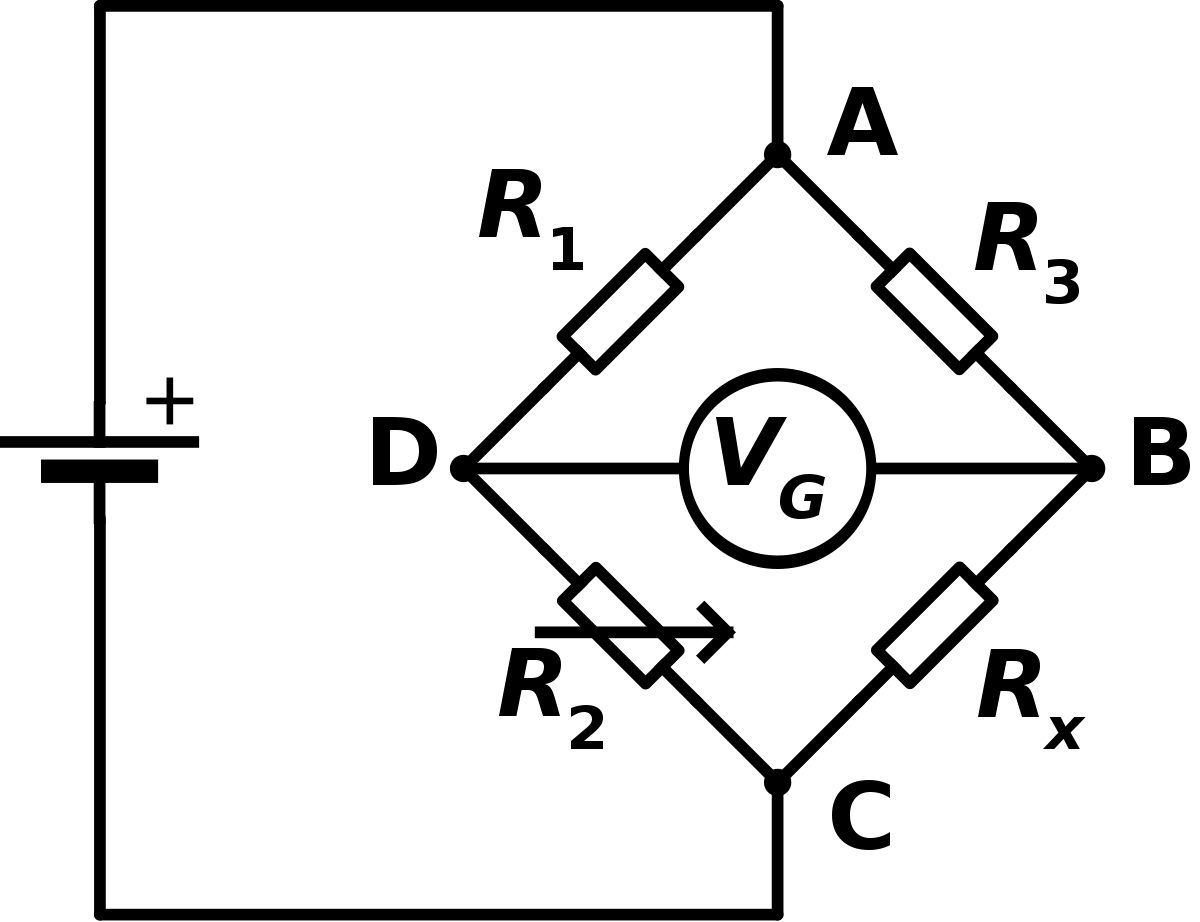
\includegraphics[width=\textwidth]{pictures/1090.png}
	\end{center}
	\fonte{https://en.wikipedia.org/wiki/Wheatstone_bridge acesso em fev 2022}
\end{figure}

A ponte de Wheatstone é normalmente utilizada em comparações e medições de resistência elétrica que variam de 1 $\Omega$ até 1 $M\Omega$ \autocite{Hollman2011}.

Utilizando as leis de kirchhoff para analisar a saída de tensão entre os pontos B e D se obtém a \autoref{eq:Eq_220}.

\begin{equation}\label{eq:Eq_220}%
\mbox{\fontsize{17.28}{21.6}\selectfont\( %
V_{out} = V_{in} \frac{R_1 R_3 - R_2 R_4}{(R_1 + R_2)(R_3 + R_4)}
\)} %
\end{equation}

onde

$E$: Tensão de saída da ponte

$V$: Tensão de excitação da ponte

$R_i$: Resistência nominal dos resistores da ponte

\hfill

Em uma aplicação onde o sensor de deformação representa uma resistência variável dentro do circuito e os outros resistores apresentam resistências
iguais ao do valor nominal do sensor utilizado, pode-se combinar a equação prévia com a equação do fator de extensão para obter uma relação entre tensão obtida
e valor de extensão apresentado no sensor, logo a equação de transferência do circuito é representada na \autoref{eq:Eq_225}.

\begin{equation}\label{eq:Eq_225}%
\mbox{\fontsize{17.28}{21.6}\selectfont\( %
\frac{V_{out}}{V_{in}} = \frac{k}{4}(\varepsilon_1 - \varepsilon_2 + \varepsilon_3 - \varepsilon_4)
\)} %
\end{equation}

onde

$V_{out}$: Tensão de saída da ponte

$V_{in}$: Tensão de excitação da ponte

$k$: Gage factor

$\varepsilon_{i}$: Valor de deformação no extensômetro "i"

\hfill

Circuitos de ponte se mostram de grande utilidade em experimentos práticos e são amplamente utilizados na medição da resistência de transdutores como extensômetros
e outros tipos de sensores que convertem uma grandeza física em uma variação de resistência. Para medições estáticas, a tensão de saída do circuito de ponte é normalmente
medido utilizando um voltímetro ou um dispositivo de coleta de dados de tensão \autocite{Hollman2011}.

Uma vez conhecido o fato de que não aconteceram grandes variações de tensão em um extensômetro na sua operação, devido ao fato do material apresentar pequenos valores de
deformação dentro de sua zona elástica, pode-se concluir que o sinal de saída da ponte de Wheatstone não será de grande ordem de grandeza, logo, deve-se estudar métodos de
amplificação dessa tensão com o objetivo de facilitar a obtenção das leituras por um voltímetro digital ou placa de controle.

\section{OBTENÇÃO DE SINAIS}

Medidas experimentais podem ocorrer de diversas formas e em vários casos os sinais são considerados fracos, logo eles devem ser amplificados com o objetivo de facilitar sua
utilização por um dispositivo de saída. A maior parte dos amplificadores de sinal atuais utilizam circuitos integrados ou dispositivos de estado sólido para amplificar um
sinal fraco analógico \autocite{Hollman2011}.

\begin{figure}[htb]
	\caption{\label{fig:1100} Princípio de funcionamento de um amplificador de sinal}
	\begin{center}
		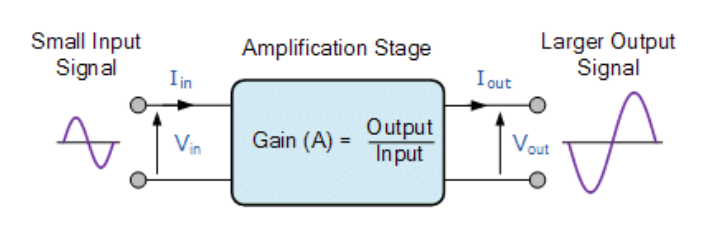
\includegraphics[width=\textwidth]{pictures/1100.png}
	\end{center}
	\fonte{https://www.electronics-tutorials.ws/amplifier/amp_1.html\\ acesso em fev 2022}
\end{figure}

O grau de amplificação de um amplificador pode ser dado pela \autoref{eq:Eq_230}, que relaciona o sinal de entrada recebido pelo amp com o sinal de saída,
que é lido pelo controlador.

\begin{equation}\label{eq:Eq_230}%
\mbox{\fontsize{17.28}{21.6}\selectfont\( %
Gain(A) = \frac{input}{output}
\)} %
\end{equation}

onde

$Gain (A)$: Grau de amplificação do amplificador de sinal

$input$: Sinal de entrada

$output$: Sinal amplificado

\hfill

Devido a efeitos aleatórios ou conhecidos ruídos característicos sempre estarão presentes em situações de tomada de medidas, esses ruídos podem ser filtrados utilizando
circuitos que apenas permitem que uma certa parte das frequências que compõem o sinal obtido passem adiante no circuito a fim de modificar o sinal de saída do amplificador.
Essa filtragem não resolve todos os problemas que podem ser encontrados, porém melhora significativamente o resultado de um experimento \autocite{Hollman2011}.

\begin{figure}[htb]
	\caption{\label{fig:1110} Ilustração de ruidos presentes em sinais analógicos e digitais}
	\begin{center}
		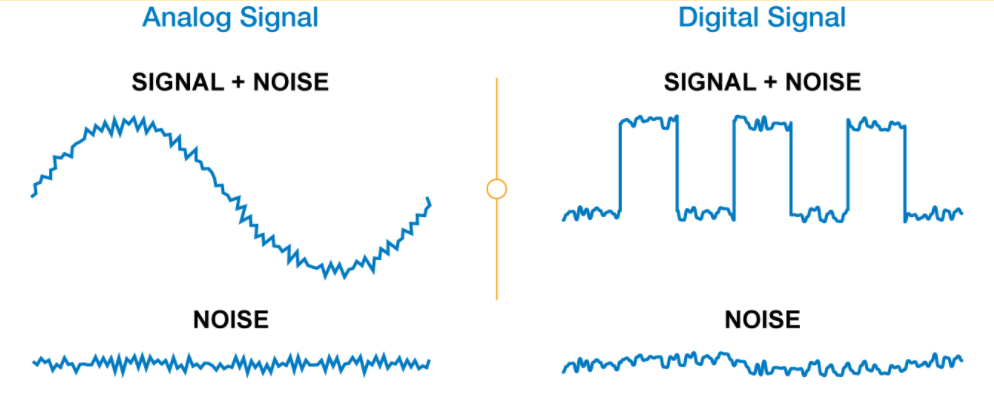
\includegraphics[width=\textwidth]{pictures/1110.png}
	\end{center}
	\fonte{www.quora.com/How-can-digital-signals-posses-noise-immunity acesso em fev 2022}
\end{figure}

Uma vez que os sinais encontrados até aqui no sistema são de característica analógica e espera-se que a utilização e tratamento deles ocorra em um computador ou placa
controladora como Arduino, que opera de maneira digital, deve-se então converter essas informações de tensão de um meio analogico para um meio digital, para isso é utilizado
um conversor digital-analógico.

\begin{figure}[htb]
	\caption{\label{fig:1120} Representação gráfica de um sinal analógico em forma digital}
	\begin{center}
		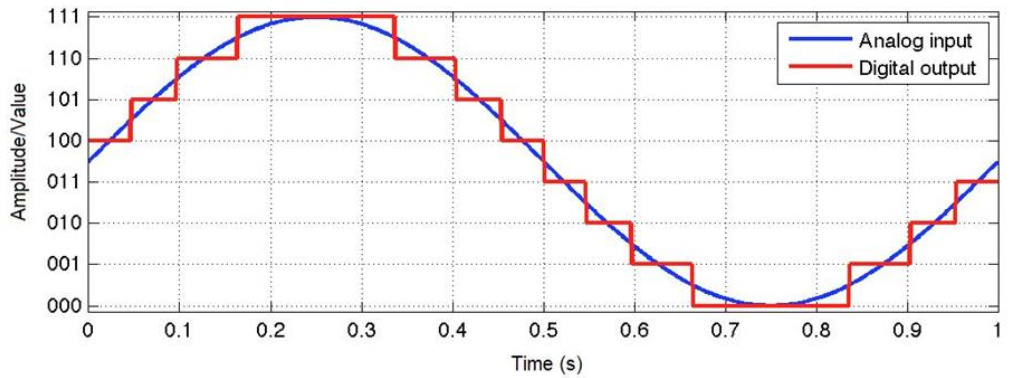
\includegraphics[width=\textwidth]{pictures/1120.png}
	\end{center}
	\fonte{{www.arrow.com/en/research-and-events/articles/engineering-resource-basics-of-analog-to-digital-converters} acesso em fev 2022}
\end{figure}

Em um meio analógico, as variáveis físicas são processadas como valores num meio contínuo, enquanto em um meio digital, valores são caracterizados por uma representação
discreta. Uma faz razões para o tratamento de sinais de maneira digital é imunizar o sinal obtido do efeito de ruídos durante a transmissão, uma vez que definir se um sinal
obtido é de valor 1 ou 0 é muito mais fácil do que definir se é um valor dentre os infinitos possíveis em um meio contínuo \autocite{Hollman2011}.

Com a finalidade de não ser perdidas informações no momento de conversão de um sinal do meio analógico para a forma digital, deve ser seguido o teorema sampling que estipula
que a taxa de leitura de um sinal de maneira digital necessita ser pelo menos duas vezes o valor da frequência desse sinal no meio analógico \autocite{Hollman2011}.

A aquisição e processamento subsequente dos sinais obtidos pode ser feito de diversas formas, desde simples cálculos e obtenção manuais de dados até utilizando
rotinas computacionais complexas. O objetivo do sistema de aquisição de dados é o de coletar, processar e/ou armazenar os dados obtidos em um experimento ou medição
\autocite{Hollman2011}.

\section{SISTEMAS DE MEDIÇÃO}

A maior parte dos sistemas de medição podem ser divididos em três partes, um estágio de detecção da medida física, um estágio intermediário de amplificação, filtragem
e conversão de sinal e um estágio final, que engloba a obtenção e processamento do sinal por um dispositivo de controle \autocite{Hollman2011}.

\begin{figure}[htb]
	\caption{\label{fig:1130} Diagrama de blocos dos estágios de um sistema de medição}
	\begin{center}
		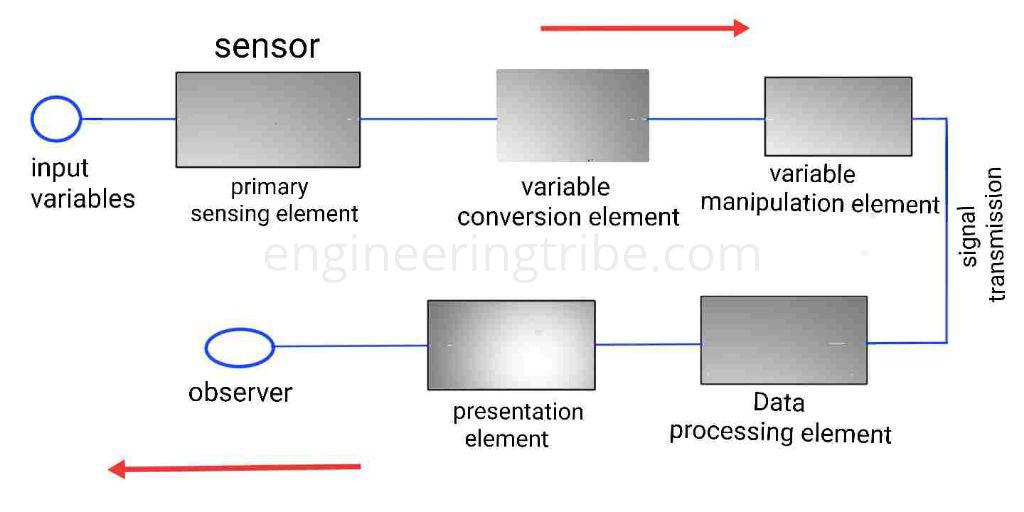
\includegraphics[width=\textwidth]{pictures/1130.jpg}
	\end{center}
	\fonte{https://www.engineeringtribe.com/2020/09/generalized-measurement-system.html\\ acesso em fev 2022}
\end{figure}

Uma medição é considerada estática quando a grandeza física analisada não apresenta mudanças no tempo como uma viga sobre uma carga constante de flexão, caso essa viga
é sujeita a um tipo de vibração, ou a um carregamento cíclico, então não pode mais se considerar o sinal estático \autocite{Hollman2011}.

Para desenvolver o sistema de controle e obtenção do sinal foi utilizado a plataforma de desenvolvimento ESP8266.
Suas principais vantagens sobre a plataforma Arduino, de menor preço e mais amplamente utilizada, é devido ao fato de que o ESP8266 apresenta em sua construção um módulo de
comunicação sem fio wifi integrado, o que reduz o tamanho do dispositivo e o torna mais barato em aplicações que necessitam de comunicação wireless \autocite{DocsESP8266}.

\begin{figure}[htb]
	\caption{\label{fig:1140} Controlador ESP8266}
	\begin{center}
		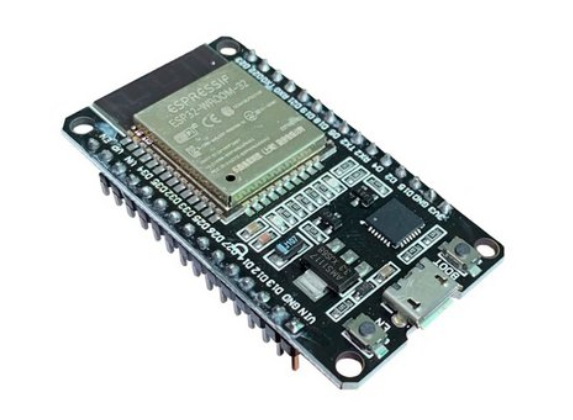
\includegraphics[width=\textwidth]{pictures/1140.jpg}
	\end{center}
	\fonte{amazon.com}
\end{figure}

A programação do controlador é feita utilizando uma linguagem de programação baseada na linguagem C + + adaptada para a utilização em placas de controle utilizando o ambiente
de desenvolvimento Arduino IDE, que permite a utilização de extensões para programação e utilização de módulos externos, como o amplificador de sinal.

O HX711 é conversor analógico digital de precisão com resolução de 24 bits, desenvolvido para utilização para balanças e aplicações de controle industriais para se conectar
diretamente com circuitos de ponte. O módulo é capaz de obter sinais na frequência de até 80 amostras por segundo e fator de ganho de 128. O amplificador de sinal que pode ser
utilizado para obtenção de sinais com tensão tão baixas quanto na faixa de ${\pm 20}{m\V}$, o que permite pequenos sinais serem medidos com alta resolução \autocite{DocsHX711}.

\begin{figure}[htb]
	\caption{\label{fig:1150} Conversor analógico digital HX711}
	\begin{center}
		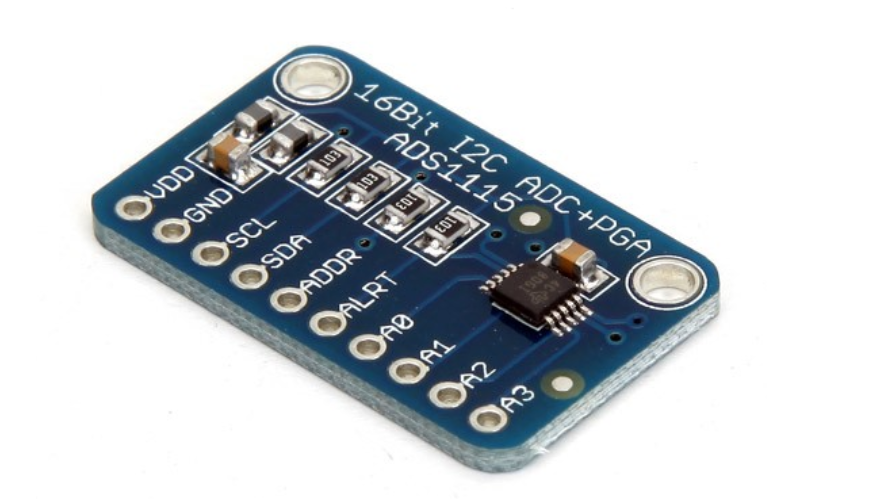
\includegraphics[width=\textwidth]{pictures/1150.jpg}
	\end{center}
	\fonte{amazon.com}
\end{figure}

Os dados obtidos pelo sistema de medição são todos em formato digital em forma de vetores unidimensionais compostos pelos valores das amostras obtidas durante o tempo do
experimento, esses valores são transmitidos em tempo real para um computador que executa um programa de obtenção de dados para realizar transformações mais complexas e
análises dos sinais obtidos em tempo real.

\section{ANÁLISE DOS SINAIS OBTIDOS}

Algum tipo de análise deve sempre ser feita em todo tipo de conjuntos de dados experimentais. Várias considerações entram na determinação final da validade dos resultados
experimentais, erros podem acarretar na invalidade dos dados mesmo quando estes foram obtidos com cautela. Alguns erros são de natureza aleatória, e outros podem ser por
natureza física ou por descuido do experimentador, como flutuações eletrônicas, fricção ou desgaste dos componentes, esses tipos de erros devem ser descartados imediatamente
\autocite{Hollman2011}.

Leituras individuais em um instrumento podem variar devido a erros de natureza aleatória, que seguem uma distribuição estatística normal, e o experimentador pode estar
desejando obter o valor médio de diversas leituras realizadas \autocite{Hollman2011}. A \autoref{eq:Eq_240} obtém o valor médio para uma medição experimental consistente
de diversas leituras.

\begin{equation}\label{eq:Eq_240}%
\mbox{\fontsize{17.28}{21.6}\selectfont\( %
\overline{x} = {\frac {1}{n}}\sum _{i=1}^{x}a_{i}
\)} %
\end{equation}

\hfill

Para cada leitura é esperado um valor de desvio lido, deve se notar que quanto melhor for o sistema de medição menor serão os valores de desvio obtidos no conjunto de
leituras, o desvio padrão, representado pela \autoref{eq:Eq_250}, se mostra como um bom indicador da situação dos desvios, e consequentemente da exatidão de um sistema de
medição.

\begin{equation}\label{eq:Eq_250}%
\mbox{\fontsize{17.28}{21.6}\selectfont\( %
\sigma = \sqrt{\frac{\Sigma(x_i-\mu)^{2}}{n}}
\)} %
\end{equation}

\hfill

Essa equação de desvio padrão deve ser utilizada para grandes populações de amostras ou para quando os dados obtidos podem ser comparados com grandezas
conhecidas \autocite{Hollman2011}. Para se obter a informação de se os valores experimentais estão de acordo com os desejados pode-se utilizar o teste do chi quadrado,
representado na \autoref{eq:Eq_260}.

\begin{equation}\label{eq:Eq_260}%
\mbox{\fontsize{17.28}{21.6}\selectfont\( %
\chi^{2} = \sum{\frac{(observed - expected)^{2}}{expected}}
\)} %
\end{equation}

\hfill

Esse teste é uma importante ferramenta de teste de qualquer resultado de distribuição experimental esperada. Se o valor de chi quadrado é igual a zero
então a distribuição assumida é exatamente a distribuição real, quanto maior o valor de chi quadrado, menor é a correlação entre os dados medidos e os reais. \autocite{Hollman2011}

\subsection{Ambiente de desenvolvimento computacional Python}

A linguagem computacional Python é utilizada tantop para desenvolvimento do software que realiza a comunicação entre o sistema de medição e o computador durante a utilização,
quanto para a criação de rotinas para obtenção dos dados estatísticos para cada amostra obtida.

Python se caracteriza como uma linguagem de programação humanamente amigável, básica e de fácil leitura e entendimento.
Que permite ao usuário a utilização de extensões e pacotes com funções de conveniência para resolver a maior parte dos problemas computacionais encontrados \autocite{TimHall2010}.

A extensão numpy é um pacote fundamental para computação científica utilizando a linguagem de programação Python. O numpy é uma ferramenta utilizada para o processamento
de dados em forma vetorial, uni ou multidimensional, seu funcionamento é baseado na conversão dos dados numéricos do formato de lista para um formato específico, altamente
otimizado chamado ndarray. O pacote numpy também apresenta diversas funções matemáticas, lógicas, estatísticas, algébricas feitas para serem utilizadas com objetos ndarray,
isso acarreta em uma minimização do tempo de processamento de um programa se comparado com utilizando funções nativas de python \autocite{DocsPandas}. As principais funções
utilizadas são demonstradas na \autoref{tab:PythonNumpy}.

\begin{table}[htb]
	\caption{Funções do pacote NumPy utilizadas}
	\label{tab:PythonNumpy}
	\resizebox{\textwidth}{!}{%
		\begin{tabular}{p{2.0cm}p{5.0cm}p{3.0cm}p{3.0cm}}
			\toprule
			\textbf{Função} & \textbf{Descrição } & \textbf{Parâmetros de entrada} & \textbf{Parâmetros de saída} \\
			\midrule
			array & Cria um objeto do numpy & Lista python & Vetor ndarray \\
			average & Obtem valor médio & Vetor ndarray & Valor médio \\
			std & Obtém desvio padrão & Vetor ndarray & Valor desvio padrão \\
			amax & Obtém valor máximo & Vetor ndarray & Valor máximo \\
			amin & Obtém valor mínimo & Vetor ndarray & Valor mínimo \\
			\bottomrule
		\end{tabular}
	}
	\fonte{O autor (2022)}
\end{table}

Uma grande gama de outros pacotes em python usam como base a estrutura de dados e funções presentes, como o pandas, que é utilizado para facilitar a manipulação e
armazenamento de dados em formato de tabular, como planilhas e bancos de dados \autocite{DocsPandas}. Dados em formatos tabulares do pandas podem facilmente ser processados,
analisados e armazenados utilizando funções do numpy e funções nativas do pandas.

Com o auxílio do processamento de dados tabulares e utilizando as funções estatísticas do pacote numpy pode-se facilmente obter os valores nominais e de erro de cada medida
tomada com o dispositivo de medição. Então deve-se partir para a fase da análise dos dados nominais obtidos.

\subsection{Análise dos valores nominais}

Uma vez obtidos todos os valores nominais para cada situação experimental analisada, devem ser criadas representações gráficas da distribuição dos resultados obtidos para
isso é utilizado o pacote scipy, que é uma coleção de algoritmos matemáticos e funções de conveniência, desenvolvidos em cima do pacote numpy. Ele proporciona ao usuário
funções e classes para manipulação e visualização de dados científicos. O pacote scipy se mostra como um forte competidor aos ambientes de desenvolvimento mais comumente
utilizados, como o Matlab, Scilab e o Octave \autocite{DocsSciPy}.

A principal visualização a ser obtida no experimento é o gráfico de distribuição de cargas aplicados pelos valores de tensão da ponte de Wheatstone obtidos, então, utilizando
o método de minimização dos quadrados, pode-se obter os parâmetros básicos que descrevem uma função matemática em que os erros entre valores observados do experimento e os
estimados sejam o mínimo o possível.

\begin{figure}[htb]
	\caption{\label{fig:1160} Regressão linear}
	\begin{center}
		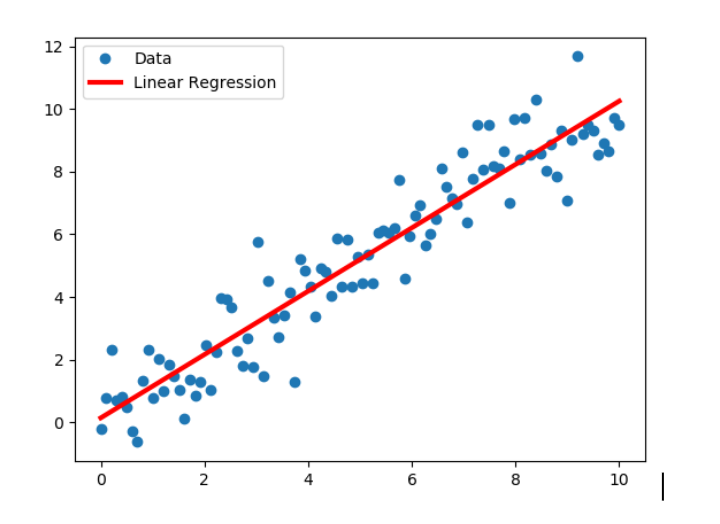
\includegraphics[width=\textwidth]{pictures/1160.png}
	\end{center}
	\fonte{www.researchgate.net/figure/Linear-Regression-model-sample-illustration_fig3_340271573 acesso em fev 2022}
\end{figure}

O gráfico de regressão linear dos dados experimentais é obtido utilizando a função scipy.lialg.regress do pacote scipy.

\section{METODOLOGIA DE DESENVOLVIMENTO DE PROJETO DE PRODUTO}

Desenvolvimento de produto entende-se como o processo de transformação de informações e conceitos até a produção e uso de um produto. Para se desenvolver um novo produto
é necessário saber o que fazer, para quem fazer, quando fazer, com que fazer e como fazer. Esta organização é denominada metodologia de projeto ou metodologia de
desenvolvimento de produtos. \autocite{Back2008}

O projeto de um produto engloba todas as etapas de definição das funções e características operacionais necessárias em um produto a ser desenvolvido, o modelo PRODIP
divide o projeto em macro etapas, cada uma contemplando uma fase do desenvolvimento de um produto, uma visão geral das etapas dessa metodologia é mostrada na \autoref{fig:1070}.
\autocite{PRODIP}.

\begin{figure}[htb]
	\caption{\label{fig:1170}Etapas da metodologia PRODIP}
	\begin{center}
		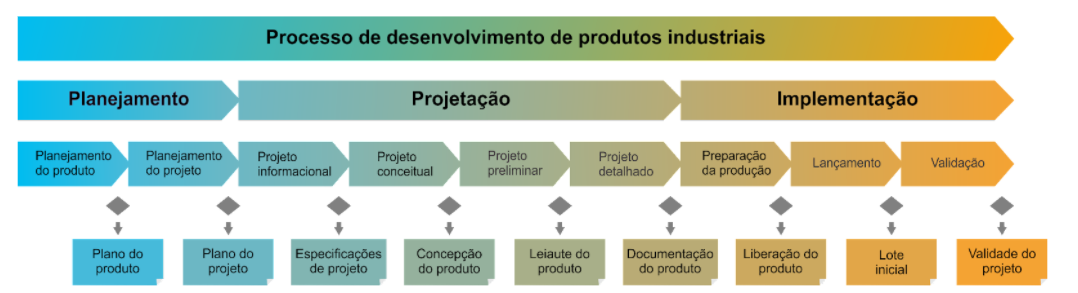
\includegraphics[width=\textwidth]{pictures/1170.png}
	\end{center}
	\fonte{\autocite{PRODIP}}
\end{figure}

Novos produtos não precisam ser necessariamente produtos totalmente originais. Um produto novo pode ser obtido pela atualização, melhorias e/ou modificações de um produto
existente, desta forma um produto existente pode ser reintroduzido a um novo nicho de mercado, e ele será considerado um novo produto. Para problemas de pequeno porte, pode
ocorrer de que não exista a necessidade de se seguir um longo e rigoroso caminho para o desenvolvimento do projeto do produto. \autocite{Back2008}

Embasado no argumento indicado por Back em sua obra, a metodologia seguida segue as etapas apresentadas na \autocite{PRODIP}, porém, nem todas as ferramentas e sub etapas
apresentadas serão rigorosamente seguidas. O autor ignorou ou simplificou algumas etapas, principalmente nas fases informacional e conceitual do projeto, uma vez que o
objetivo deste trabalho não é o de gerar um produto pronto para produção em massa.

\subsection{Fase de planejamento}

A fase de planejamento do projeto visa definir as etapas de desenvolvimento das ideias selecionadas utilizando definições de escopo, cronograma, orçamento riscos etc.
Nessa etapa são definidas as ideias do problema e produto, então é feito um mapeamento tecnológico, em que, segundo a metodologia "são organizadas as informações do mercado,
produto e tecnologia ao longo do tempo.  Essas informações são correlacionadas e servem de base para estabelecer o plano de produtos." \autocite{PRODIP}.

O resultado da fase de planejamento do projeto é um documento que contém informações relacionadas ao escopo do projeto, como o problema a ser resolvido e as ideias base de
resolução do problema. O escopo elaborado é o principal guia que direciona o desenvolvimento do produto e de suas funcionalidades. As próximas etapas apresentadas do projeto
servem para solucionar metodologicamente o problema base definido no escopo.

\subsection{Projeto informacional}

Nessa fase o objetivo é o estabelecimento das especificações de projeto, as quais irão orientar o desenvolvimento técnico do produto. O principal método empregado é a matriz
da casa da qualidade da metodologia QFD (Quality Function Deployment). O projeto informacional utiliza ferramentas para definição de especificações de projeto que irão
orientar o desenvolvimento do produto, o principal é a matriz QFD, utilizada para definir a importância dos requisitos do produto.  \autocite{PRODIP}

\begin{figure}[htb]
	\caption{\label{fig:1180}Etapas do projeto informacional}
	\begin{center}
		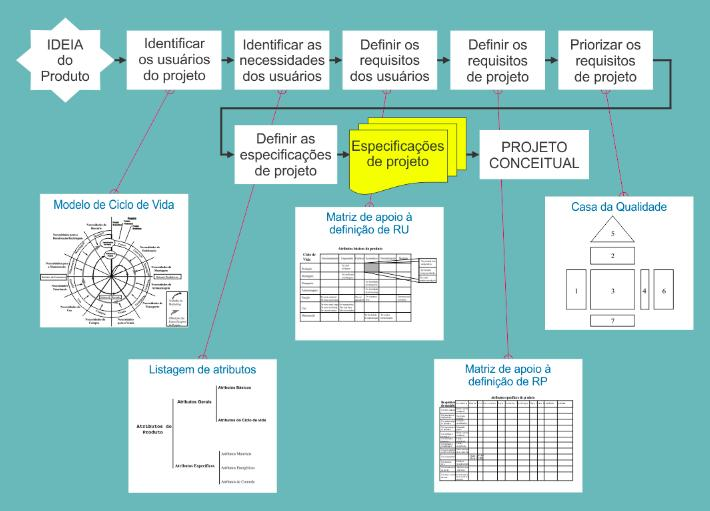
\includegraphics[width=\textwidth]{pictures/1180.jpg}
	\end{center}
	\fonte{\autocite{PRODIP}}
\end{figure}

No final do projeto informacional, é obtido de maneira clara e organizada quais são os requisitos do cliente em relação ao produto que está em desenvolvimento e quais são as
funções o produto necessários que o produto necessita ter a fim de realizar os requisitos do cliente. Também se obtém, de forma quantizada, a ordem de prioridade nas quais
o projeto necessita realizar os requisitos.

\subsection{Projeto conceitual}

Nesta etapa do projeto inicia-se o projeto e desenvolvimento das soluções conceituais para se atingir os requisitos obtidos na etapa anterior, o projeto conceitual é
caracterizado pela fase criativa onde são geradas e avaliadas técnica e economicamente as alternativas para resolução do problema. Dentre as ferramentas utilizadas nessa
fase se destacam matriz síntese de funções, matriz morfológica e matrizes multicritério de seleção. \autocite{PRODIP}

\begin{figure}[htb]
	\caption{\label{fig:1190}Etapas do projeto conceitual}
	\begin{center}
		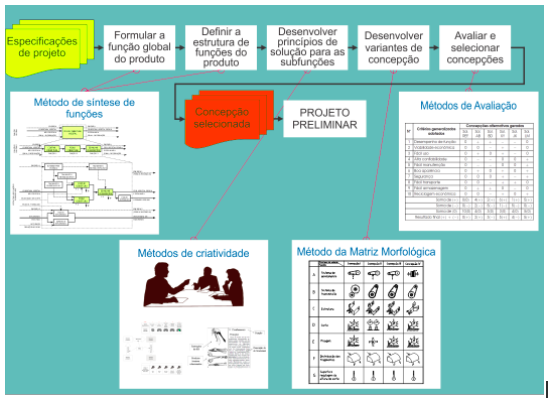
\includegraphics[width=\textwidth]{pictures/1190.png}
	\end{center}
	\fonte{\autocite{PRODIP}}
\end{figure}

\subsection{Projeto preliminar}

No projeto preliminar é definido a forma final do produto, nessa fase são definidas características geométricas, de montagem, materiais para fabricação, características
ergonômicas e de segurança e processos de manufatura do produto. Também pode ser realizados testes com protótipos para prova de conceito e otimização das características
do produto desenvolvido até essa fase. \autocite{Back2008}

Os resultados dessa fase são as documentações de viabilidade econômica e requisitos de manufatura, e um protótipo funcional do produto.

\subsection{Projeto detalhado}

A elaboração do projeto detalhado se destina a vários propósitos, como a aprovação do protótipo, a finalização das especificações dos componentes e o detalhamento do plano
de manufatura. \autocite{Back2008}

Nessa fase são gerados as documentações de especificação dos componentes, como desenhos técnicos, esquemas elétricos, planos de manufatura e softwares utilizados. Nesta fase
são feitos testes em campo e laboratório e acontece a otimização do protótipo com objetivo de preparação para produção.


    % Capitulo de revisão de literatura
    \phantomsection

\chapter{Desenvolvimento}

O presente capítulo é dividido em duas fases, a primeira apresenta o desenvolvimento e os resultados das etapas da metodologia de desenvolvimento do protótipo do dispositivo.
E a segunda seção apresenta a metodologia do experimento utilizado como prova de conceito do dispositivo desenvolvido.

\section{Planejamento do projeto}

O problema a ser solucionado é o de difícil acesso e altos custos para a obtenção de dados de deformação em tempo real.
A primeira etapa para realizar o planejamento do projeto foi uma pesquisa de custo e disponibilidade de produtos iguais ou semelhantes a este propósito no mercado digital,
os resultados da pesquisa são apresentados na próxima subseção.

\subsection{Mapeamento tecnológico}

Foram encontrados inúmeros dispositivos para telemetria e obtenção de sinais de sensores para aplicações industriais, de alta performance, ou para aplicações muito específicas,
estes foram ignorados devido devido a altos custos ou baixa flexibilidade em relação ao dispositivo proposto. Dos produtos encontrados, três se mostraram mais semelhantes ao que será desenvolvido.

A empresa Isso disponibiliza em sua loja virtual Dois dispositivos para controle e obtenção de dados, denominados dmi tcr 44es, mostrado na \autoref{fig:2010}, e dmi tcr 88es.
Segundo o fabricante esses dispositivos são utilizados para aplicações de acionamentos e telemetria remota, e são indicados para uso em automações residenciais e industriais,
a única diferença observada entre os dois modelos são o número de entradas e saídas de sinais que o dispositivo possui. \autocite{Isso44es}

\begin{figure}[htb]
	\caption{\label{fig:2010} Datalogger DMI TCR 44es}
	\begin{center}
		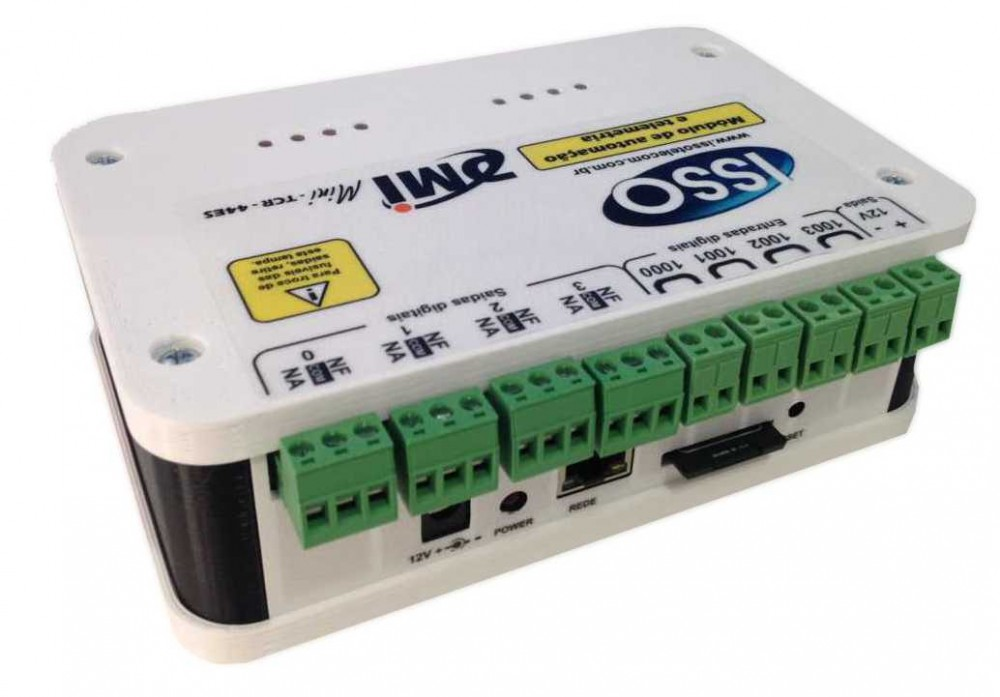
\includegraphics[width=\textwidth]{pictures/2010.jpg}
	\end{center}
	\fonte{\autocite{Isso44es}}
\end{figure}

Outro dispositivo, denominado Bridge101A, mostrado na \autoref{fig:2030}, fabricado pela empresa Madgetech foi encontrado, segundo a empresa é um data logger compacto que mede e armazena valores de tensões elétricas,
e é normalmente utilizado com extensômetros, células de carga e outras sensores de baixa tensão, e que o dispositivo é utilizado para calcular com precisão parâmetros de tensão, torque, deformação
e pressão ao longo do tempo. \autocite{Bridge101A}

\begin{figure}[htb]
	\caption{\label{fig:2030} Dispositivo Bridge101A}
	\begin{center}
		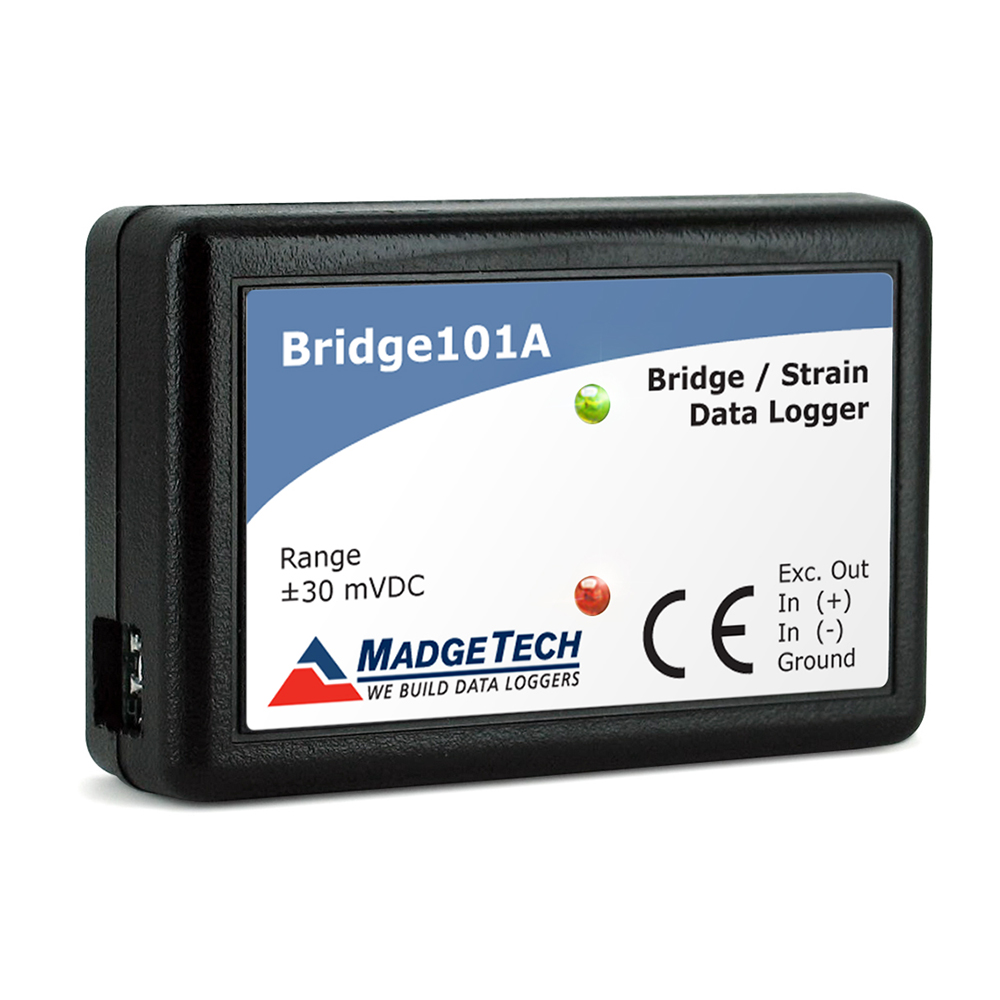
\includegraphics[width=\textwidth]{pictures/2030.jpg}
	\end{center}
	\fonte{\autocite{Bridge101A}}
\end{figure}

A \autoref{tab:Banchmarking} mostra uma comparação entre os dados de utilização obtidos pela documentação dos dois dispositivos previamente apresentados.

\begin{table}[!ht]
    \caption{Benchmarking entre dispositivos encontrados}
    \label{tab:Banchmarking}
    \centering
    \resizebox{\linewidth}{!}{%
        \begin{tabular}{ l | c c r } \toprule
         			  & Isso DMI TCR 44es & Isso DMI TCR 88es & Madgetech Bridge101A \\
			\midrule
			Dimensões & 124x117x55mm & 190x117x55mm & 36x64x16mm \\
			Comunicação com PC & Conexão Ethernet & Conexão Ethernet & Conexão USB \\
%			Interface com o usuário & Software próprio & Software próprio & Software próprio \\
%			Programação & Software próprio & Software próprio & Software próprio \\
			Taxa de leitura & Não disponiblizado & Não disponiblizado & $\SI{4}{\hz}$ \\
			Faixa de tensão de leitura & Não disponiblizado & Não disponiblizado & $\SI{\pm 30}{\mV}$ \\
			Faixa de preço & R\$1100,00 & R\$1300,00 & R\$2800,00 \\
            \bottomrule
        \end{tabular}}
\fonte{O autor 2022}
\end{table}

Dentre os valores apresentados na tabela fica claro os altos preços envolvidos em qualquer aplicação que necessite a utilização desse tipo de dispositivo.
Muitos deles necessitam ainda de programas para programação e utilização proprietários e que ainda tem custos adicionais para utilização. O dispositivo desenvolvido neste trabalho tem como objetivo um preço
consideravelmente menor que os analisados e programável e utilizável utilizando tecnologias gratuitas e de código aberto.

\subsection{Pesquisa científica}

Com o intuito de facilitar o desenvolvimento do dispositivo, foi realizada uma revisão sistemática de trabalhos científicos e acadêmicos disponíveis nas bases de dados Web of Science, Springer,
Sciencedirect e Google Scholar, utilizando como palavras-chave “Dynamic, Torque, Shaft, Sensor, Strain, Gauge”, os principais obtidos são apresentados nessa subseção.

Um artigo desenvolvido por \autocite{Niedworok2014} relata o desenvolvimento e aplicação de um sistema de sensoriamento de torque em tempo real em um eixo cardan de um carro de mina utilizando a medição
da deformação utilizando extensômetro com transferência dos dados via radiofrequência, o trabalho também indica que o posicionamento do sensor necessita estar em contato com a superfície de maior deformação do componente,
o autor realiza uma análise por elementos finitos para encontrar esse local. O artigo também aponta que o sinal vindo do sensor deve ser ampliado utilizando uma ponte de Wheatstone para conseguir ter a instrumentação
correta da grandeza. O artigo mostrou resultados satisfatórios e não discutiu sobre ruídos e imprecisões presentes nos dados obtidos.

\autocite{Nurprasetio2018} desenvolve, em seu trabalho, um sistema de medição para veículos terrestres, aplicado em uma bancada de testes que simula o estado de veículos terrestres em operação, o sistema
utiliza um microprocessador Arduino nano de fácil acesso e baixo custo. Os dados são transmitidos via comunicação bluetooth. O artigo também ilustra o processo de calibração do dispositivo feito antes do teste dinâmico,
assim como no trabalho anterior, também é enfatizada a necessidade das metodologias de instrumentação do sinal vindo do extensômetro. Seus resultados também se mostraram promissores, porém o autor indica que é necessário
a remoção dos ruídos de medição, o que segundo ele será endereçado em um trabalho futuro.

\autocite{Gharghan2017} compara um sistema de medição similar ao dos dois trabalhos prévios com um sistema de medição de torque em tempo real de alto custo utilizado por ciclistas profissionais no pedivela.
O artigo introduz a tecnologia de transmissão de dados Zigbee, que consegue transmitir dados a um baixo consumo energético. Após a obtenção dos dados, o autor utiliza as ferramentas de análise estatística de Bland-Altman
e porcentagem de erro médio absoluto para a validação do sistema.

\autocite{Silva2017} compara os dados de um sistema semelhante aos anteriores com resultados de análises de modelo matemático analítico e análise por elementos finitos aplicados em bancadas de viga engastada com carga
na ponta e de torque aplicado em um eixo com um dos lados travados, diferente dos trabalhos anteriores, este possui uma seção com o desenvolvimento das equações dos modelos utilizados, e assim como os artigos anteriores
foram encontrados resultados satisfatórios.

Com os dados do mapeamento tecnológico e da revisão dos trabalhos científicos recentes, é elaborado um documento de escopo base do projeto com o conceito de funcionamento básico e uma descrição dos componentes
necessários e seus respectivos preços, esse escopo está disponível no apêndice A.

\section{Projeto informacional}

%Definição do público alvo
%
%Formulário de pesquisa
%
%Matriz de requisitos do cliente
%
%Matriz de requisitos do projeto
%
%Matriz QFD

\section{Elaboração do conceito}

%Matriz morfológica
%
%Comparação e benchmarking
%
%Placa de controle:	Opções	Vantagens e desvantagens de cada uma	Qual foi a escolhida	Preços

\begin{table}[!ht]
    \caption{Características de ganho para o ADS1115}
    \label{tab:ads1115modes}
    \centering
    \resizebox{\textwidth}{!}{%
        \begin{tabular}{ l | c c r } \toprule
         	Ganho & Faixa de leitura & Resolução \\
			\midrule
			 2/3x & ${\pm 6.144}V$ & $1bit$ = ${0.1875}{m}V$ \\
			 1x & ${\pm 4.096}V$ & $1bit$ = ${0.125}{m}V$ \\
			 2x & ${\pm 2.048}V$ & $1bit$ = ${0.0625}{m}V$ \\
			 4x & ${\pm 1.024}V$ & $1bit$ = ${0.03125}{m}V$ \\
			 8x & ${\pm 0.512}V$ & $1bit$ = ${0.015625}{m}V$ \\
			 16x & ${\pm 0.256}V$ & $1bit$ = ${0.0078125}{m}V$ \\
            \bottomrule
        \end{tabular}}
\fonte{O autor 2022}
\end{table}

%
%amplificador: Opções	Vantagens e desvantagens de cada uma	Qual foi a escolhida	Preços

\section{Preparação do protótipo}



\section{Validação do protótipo}

A metodologia de execução do experimento para validar o funcionamento do protótipo desenvolvido segue a mesma metodologia do experimento realizado no trabalho de conclusão
de curso de \autocite{Minela2017}, uma introdução aos principais tópicos dessa metodologia e eventuais diferenças entre os dispositivos utilizados nos dois trabalhos para cada tópico é feita nessa seção.

Os ensaios realizados envolvem a leitura de extensômetros colados em corpos de prova sobre ação de cargas específicas. Um dispositivo de análise de cargas de flexão e
um para cargas em torção foram desenvolvidos e produzidos por \autocite{Minela2017}, os mesmos dispositivos foram utilizados para este trabalho.

\subsection{Dispositivo para ensaio de flexão}

O dispositivo para realizar o ensaio de flexão é composto por uma viga de seção retangular de $20mm$ de largura por $2mm$ de espessura, que mede $200mm$
de comprimento e é de uma liga desconhecida de alumínio, e uma base projetada e fabricada em aço 1020 para fixar a viga em uma situação de engaste na viga.
A imagem mostra o projeto do dispositivo desenvolvido por \autocite{Minela2017}.

\begin{figure}[htb]
	\caption{\label{fig:2040} Dispositivo de ensaio de flexão}
	\begin{center}
		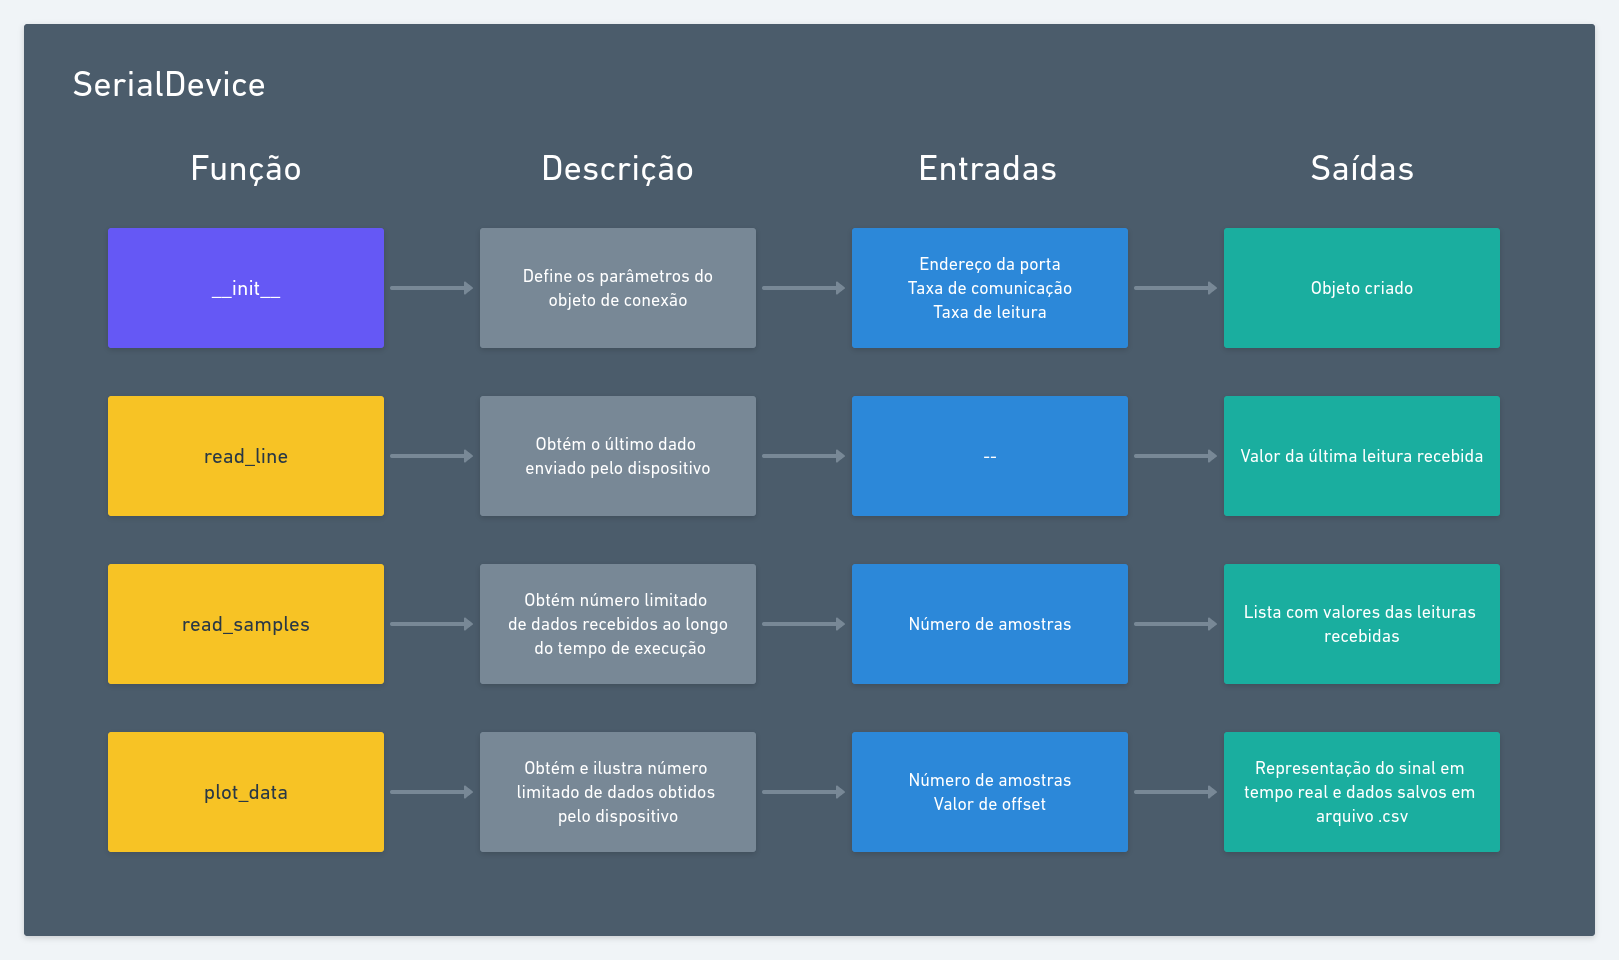
\includegraphics[width=\textwidth]{pictures/2040.png}
	\end{center}
	\fonte{\autocite{Minela2017}}
\end{figure}

Na viga é colado um extensômetro unidimensional para obter os dados de deformação, as propriedades do extensômetro utilizado são mostradas na
\autoref{tab:PropriedadesExtensometro}.

\begin{table}[htb]
\caption[]{Propriedades do extensômetro colado ao dispositivo de flexão}
\label{tab:PropriedadesExtensometro}
\resizebox{\textwidth}{!}{%
\begin{tabular}{p{6.5cm}p{8cm}}
	\toprule
	Marca & Micro Measurements \textregistered \\
	Tipo de extensômetro & EA-06-250AF-120 \\
	Resistência Elétrica & ${120\pm 0.15\% \Omega}$ \\
	Factor de gage até ${75 ^\circ F}$ & ${2.025 \pm 0.5 \%}$ \\
	Comprimento & ${6.35} \mm$ \\
	Limite de têmperatura & ${-75\tccentigrade}$ á ${175\tccentigrade}$ para medições estáticas \\
	\bottomrule
\end{tabular}
}
\fonte{Adapdato de \autocite{Minela2017}}
\end{table}

As cargas são aplicadas na extremidade livre da viga a distância de 150mm entre o centro do extensômetro e o ponto de aplicação da carga.
Com a finalidade de se obter os valores de deformação causados pela aplicação de cada carga, cada trabalho utiliza-se de um sistema de medição diferente, apresentado
na seção seguinte.

\subsection{Sistemas de medição}

Tanto o sistema de medição utilizado em \autocite{Minela2017} quanto o utilizado para o desenvolvimento deste trabalho seguem o mesmo princípio de funcionamento.

\begin{figure}[htb]
	\caption{\label{fig:2050} Sistema de medição utilizado por \autocite{Minela2017}}
	\begin{center}
		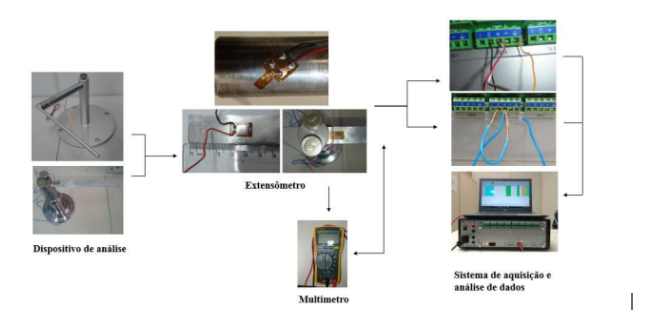
\includegraphics[width=\textwidth]{pictures/2050.png}
	\end{center}
	\fonte{\autocite{Minela2017}}
\end{figure}

O sistema de medição utilizado por \autocite{Minela2017} é composto por um dispositivo de obtenção de dados ADS2002, desenvolvido e fabricado pela LYNX Tecnologia,
que é conectado a um computador. O ADS2002 obtém os dados gerados pelo sensor e os envia ao computador via conexão ethernet.
O computador utiliza o software AQDados para conexão com o ADS2002, calibração e aferição dos extensômetros, e o softwre AqAnalysis para fazer o processamento dos sinais
e gerar relatórios de análise, ambos os programas são desenvolvidos pela fabricante do dispositivo de obtenção de dados.

\begin{figure}[htb]
	\caption{\label{fig:2060} Sistema de de medição utilizando o LINX ADS2002}
	\begin{center}
		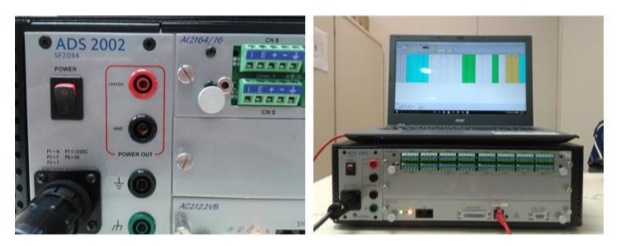
\includegraphics[width=\textwidth]{pictures/2060.png}
	\end{center}
	\fonte{\autocite{Minela2017}}
\end{figure}

A conexão entre o dispositivo de obtenção de dados e o extensômetro ocorre utilizando os terminais elétricos do canal específico de análise, o ADS2002 já possui,
integrado em si, os componentes elétricos do circuito da ponte de wheatstone para a instrumentação do sinal.
A calibração do extensômetro afim dos resultados serem mostrados como valores deformação, ao invés de tensões, é feita utilizando a \autoref{eq:Eq_270} que define um valor de
fator de engenharia em função do fator gage $FG$ da resistência média do extensômetro $RM$, resistência de calibração $RC$, que é disponibilizada pelo fabricante.

\begin{equation}\label{eq:Eq_270}%
\mbox{\fontsize{17.28}{21.6}\selectfont\( %
VE = \left ( \frac{1}{FG}\left ( \frac{RM}{RM + RC} \right ) \right )
\)} %
\end{equation}

\newline

O sistema de medição utilizando o protótipo desenvolvido pelo autor é feito pela conexão entre o controlador ESP 32 e o computador via o software desenvolvido em python
para realizar a transferência dos dados obtidos entre o controlador e o computador em tempo real.

\begin{figure}[htb]
	\caption{\label{fig:2070} Protótipo do dispositivo desenvolvido conectado com o extensometro no dispositivo de flexão}
	\begin{center}
		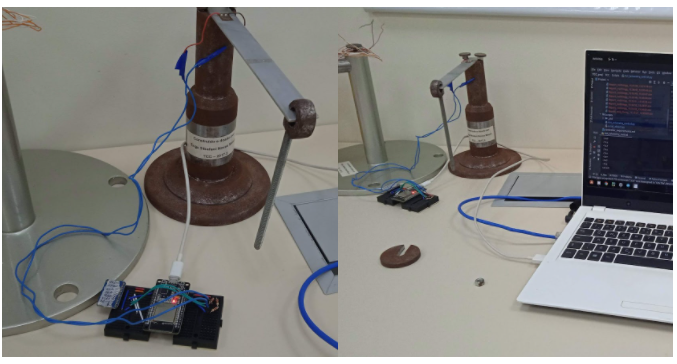
\includegraphics[width=\textwidth]{pictures/2070.png}
	\end{center}
	\fonte{O autor 2021}
\end{figure}

A calibração do dispositivo desenvolvido pelo autor é feita utilizando os sinais resultantes da aplicação de duas massas distintas conhecidas.
Os valores nominais obtidos nos sinais alimentam a \autoref{eq:Eq_280} que é utilizada para converter os valores discretos obtidos em bits pelo
amplificador de sinal para um valor de gradeza física desejado.

\begin{equation}\label{eq:Eq_280}%
\mbox{\fontsize{17.28}{21.6}\selectfont\( %
F(W) = \frac{output_{high}-output_{low}}{W_{high}-W_{low}}(W - W_{low}) + output_{low}
\)} %
\end{equation}

onde

$F(W)$: Função de calibração

$W$: Valor nominal do sinal

$W_{high}$: Carga de calibração de massa alta

$W_{low}$: Carga de calibração de massa baixa

$output_{high}$: Valor nominal do sinal obtido pela aplicação da carga alta

$output_{high}$: Valor nominal do sinal obtido pela aplicação da carga baixa

\hfill

A calibração ocorre por um método automatizado implementado no software de comunicação entre o controlador e o computador.
Após calibrado, o dados são mostrados como os valores de grandeza física calibrada.

\subsection{Cargas aplicadas}

\autocite{Minela2017} utiliza pesos com massas pré definidas apoiadas utilizando um fuso de fixação para aplicação das cargas no ponto “F” no dispositivo, mostrado na figura.
Dentre as massas utilizadas por \autocite{Minela2017} duas não foram localizadas pelo autor deste trabalho, com a finalidade de poder se obter resultados que se possam fazer
comparações diretas entre os trabalhos foram substituidas as massas não encontradas por massas semelhantes.

Todos os valores de massa dos pesos utilizados foram obtidos novamente pelo autor utilizando o valor médio de três leituras obtidas por uma balança de precisão disponibilizada pelo laboratório de metrologia
da UFSC Joinville. Os valores obtidos são apresentados na \autoref{tab:MassasUtilizadas}.

\begin{table}[!ht]
    \caption{Valores de massas utilizadas para aplicação das cargas nos dispositivos de flexão e torção}
    \label{tab:MassasUtilizadas}
    \centering
    \resizebox{\linewidth}{!}$ \\
            Fuso & $\SI{48.63}{\g}$ & $\SI{48.78}{\g}$ & $\SI{0.31}{\%}$ \\
            Peso 1 & $\SI{86.73}{\g}$ & $\SI{99.68}{\g}$ & $\SI{12.99}{\%}$ \\
            Peso 2 & $\SI{198.38}{\g}$ & $\SI{198.36}{\g}$ & $\SI{0.01}{\%}$ \\
            Peso 3 & $\SI{997.13}{\g}$ & $\SI{997.3}{\g}$ & $\SI{0.02}{\%}$ \\
            Peso 4 & $\SI{497.66}{\g}$ &$\SI{497.69}{\g}$ & $\SI{0.02}{\%}$ \\
            Peso 5 & $\SI{495.25}{\g}$ & $\SI{496.22}{\g}$ & $\SI{0.20}{\%}$ \\
            \bottomrule
        \end{tabular}}
\fonte{O autor 2022}
\end{table}

As massas da porca e do “peso 1” utilizados em \autocite{Minela2017} variam de forma considerável em relação aos pesos utilizados neste trabalho, então para todas as comparações diretas de
resultados experimentais obtidos entre os dois trabalhos deve ser aplicados fatores de correção de 11.42g para a porca e 12.95g para o “peso 1”.

O método de aplicação de cargas é caracterizado pela aplicação na extremidade livre da viga das massas utilizando o fuso como suporte, a Figura mostra a viga de aluminio defletida pela aplicação da carga do "peso 3".

\begin{figure}[htb]
	\caption{\label{fig:2080} Aplicaçao do 'peso 3' no dispositivo de flexão}
	\begin{center}
		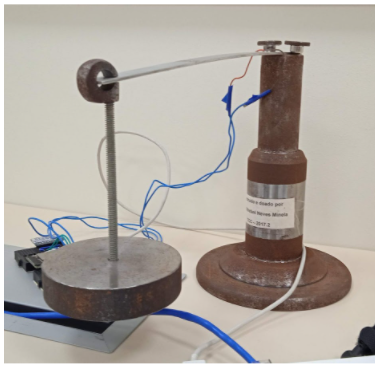
\includegraphics[width=\textwidth]{pictures/2080.png}
	\end{center}
	\fonte{O autor 2021}
\end{figure}

Na extremidade da viga encontra-se uma demarcação para auxiliar o posicionamento do apoio do fuso e as cargas são aplicadas de maneira cuidadosa de modo que não sejam geradas forças de impulso na viga.
O sistema de medição obtem valores em bits proporcionais a carga aplicada no experimento.

Os valores obtidos em bits são posteriormente convertidos em valores de carga, ou de deformação utilizando uma função de transferencia obtida pelo método de calibração.


    % Primeiro capitulo de Resultados
    
\phantomsection

\chapter{Resultados}\label{ch:capitulo_resultados}

Este capítulo apresenta os sinais e valores obtidos no experimento realizado no dispositivo de flexão.
Os tópicos aqui analisados apresentam a comparação dos resultados obtidos pelo experimento realizado pelo autor com os valores obtidos pelo
estudo de caso feito por Minela (2017).

O objetivo primário da comparação dos resultados é o de se obter dados descritivos de desempenho do dispositivo desenvolvido em relação a um sistema de medição industrial
homologado, no final do capítulo são indicados as situações de melhor desempenho do protótipo.

\section{Sinais obtidos}

Os sinais captados pelo sistema de medição desenvolvido seguem um formato trapezoidal, onde as zonas iniciais e finais representam os momentos em que a viga não se encontrava
sob a aplicação da carga, e a zona intermediária representa a total aplicação da carga no dispositivo.

\subsection{Sinais de calibração}

A primeira etapa da utilização do dispositivo é definir os sinais de calibração, para isso é obtido as respostas de leitura do módulo de conversão de sinal para a aplicação das cargas
de 0,138kg e 1,04kg, que representavam o menor e o maior peso disponível para o experimento, sem considerar as combinações.

Foi obtido o valor médio de 190 unidades discretas na zona superior do sinal trapezoidal na aplicação da massa de 0,138kg, como mostrado na \autoref{fig:4100}.
Para a aplicação da massa de 1.04kg foi obtido o valor de 612 unidades discretas, mostrado na \autoref{fig:420}.

\begin{figure}[H]
	\caption{\label{fig:4100} Sinal obtido pela aplicação da carga de 0,138kg no dispositivo}
	\begin{center}
		\includegraphics[width=350]{pictures/signals/cal_signal_1.png}
	\end{center}
	\fonte{O autor 2022}
\end{figure}

\begin{figure}[H]
	\caption{\label{fig:420} Sinal obtido pela aplicação da carga de 1,04kg no dispositivo}
	\begin{center}
		\includegraphics[width=350]{pictures/signals/cal_signal_2.png}
	\end{center}
	\fonte{O autor 2022}
\end{figure}

Uma vez obtidos os valores discretos para cada ponto de calibração e conhecidos os seus valores de deformação teóricos, é calculado os fatores $ fa $ e $ fb $ da função de interpolação
linear que converte valores obtidos pelo módulo de conversão de sinal em unidades discretas para valores equivalentes de deformação no extensômetro.
O valor do fator a encontrado foi de $ 2.8881*10^{-6} $ e o de b foi de $ -363.4311*10^{-6} $.

Uma vez definidos os parâmetros de calibração são feitos os experimentos aplicando a carga de cada peso no dispositivo de flexão.
Alguns dos sinais obtidos e uma discussão geral sobre eles são discutidos nas seções a seguir.

\subsection{Sinais calibrados obtidos}

O experimento é realizado obtendo os sinais calibrados obtidos pelo dispositivo na aplicação de cada uma das massas disponíveis e pela aplicação de combinações entre essas massas,
os valores de cargas aplicadas para a realização dos experimentos são mostradas na \autoref{tab:Cargasaplicadas}.

\begin{table}[H]
    \caption{Cargas aplicadas para os experimentos}
    \label{tab:Cargasaplicadas}
    \centering
    \resizebox{350}{!}{%
        \begin{tabular}{ l c r } \toprule
			Pesos aplicados & {Massa aplicada (Considerando fuso e porca)} \\
			Peso 1 & ${138.42} {g} $ \\
			Peso 2 & ${250.07} {g} $ \\
			Peso 3 & ${1048.82} {g} $ \\
			Peso a & ${549.35} {g} $ \\
			Pesos 1 e 2 & ${336.8} {g} $ \\
			Pesos 1 e a & ${636.08} {g} $ \\
			Pesos 2 e a & ${747.73} {g} $ \\
			Pesos 1, 2 e a & ${834.46} {g} $ \\
			Pesos 3 e 1 & ${1135.55} {g} $ \\
			Pesos 3 e 2 & ${1247.2} {g} $ \\
			Pesos 3, 2 e 1 & ${1333.93} {g} $ \\
            \bottomrule
        \end{tabular}}
\fonte{O autor 2022}
\end{table}

O primeiro peso aplicado é o de menor massa disponível, que ja tinha sido previamente utilizada para utilização na calibração do dispositivo,
o sinal obtido é mostrado na \autoref{fig:41002}, o valor de deformação obtido foi de $ 182.42 {\mu}m/m $.

\begin{figure}[H]
	\caption{\label{fig:41002} Sinal obtido da aplicação de 0,138 kg de carga aplicada no dispositivo}
	\begin{center}
		\includegraphics[width=350]{pictures/signals/w1.png}
	\end{center}
	\fonte{O autor 2022}
\end{figure}

O sinal equivalente obtido por Minela (2017) é mostrado na \autoref{fig:4102_m}.

\begin{figure}[H]
	\caption{\label{fig:4102_m} Sinal obtido da aplicação da massa de 0,163 kg de carga aplicada no dispositivo indústrial}
	\begin{center}
		\includegraphics[width=350]{pictures/signals/wp1.png}
	\end{center}
	\fonte{\autocite{Minela2017}}
\end{figure}

Uma comparação direta de valor não pode ser feita considerando os dois sinais, uma vez que as massas aplicadas não foram as mesmas, porém, analisando os sinais
pode-se notar que o efeito dos ruídos no dispositivo desenvolvido é consideravelmente menor do que os obtidos pelo dispositivo utilizado em Minela (2017).
Foi constatado que os dados apresentados por Minela (2017) foram obtidos sem a ativação dos métodos de redução de ruídos disponíveis no dispositivo Lynx ADS2002,
logo, pode-se concluir que a atuação dos filtros de passa-altas do módulo de conversão de sinal utilizado no dispositivo desenvolvido é o principal motivo pelos quais
os ruídos em todos os resultados obtidos pela utilização do protótipo desenvolvido se mostraram de baixas amplitudes.

O sinal obtido pela aplicação do de 1,04kg é mostrado na \autoref{fig:4109}, o valor de deformação obtido foi de $ 1421.41 {\mu}m/m $.

\begin{figure}[H]
	\caption{\label{fig:4109} Sinal obtido da aplicação de 1,040 kg de carga aplicada no dispositivo}
	\begin{center}
		\includegraphics[width=350]{pictures/signals/w8.png}
	\end{center}
	\fonte{O autor 2022}
\end{figure}

O sinal equivalente obtido por Minela (2017) é mostrado na \autoref{fig:4109_m}

\begin{figure}[H]
	\caption{\label{fig:4109_m} Sinal obtido da aplicação da massa de 0,163 kg de carga aplicada no dispositivo indústrial}
	\begin{center}
		\includegraphics[width=350]{pictures/signals/wp3.png}
	\end{center}
	\fonte{\autocite{Minela2017}}
\end{figure}

Assim como no primeiro sinal, nota-se que os sinais são semelhantes, com a exceção dos ruídos, que são mais impactantes com 
a utilização do dispositivo utilizado por Minela (2017) do que com a utilização do protótipo desenvolvido.

Os sinais obtidos para cada carga utilizada no experimento podem ser encontrados no \autoref{ch:sinais-obtidos}.

\subsection{Comparação dos valores de deformação experimentais e analíticos}

Utilizando a \autoref{eq:Eq_201} pode-se obter analiticamente valores de deformação esperados para cada situação de carga do experimento.
O valor de módulo de elasticidade utilizado no modelo analítico foi de $ 85.19 GPa $, que foi obtido experimentalmente no trabalho de Minela (2017)
para o mesmo dispositivo utilizado.
A \autoref{tab:ResultadosDeformacao} mostra os resultados de valores de deformação obtidos para cada experimento, os valores de deformação esperados
calculados e os valores de erro de cada resultado obtido em relação ao teórico.

\begin{table}[H]
    \caption{Resultados de deformação obtidos}
    \label{tab:ResultadosDeformacao}
    \centering
    \resizebox{350}{!} $ \\
			$ {250.07} {g} $ & $ {334.77} {\mu}m/m $ & $ {358.59} {\mu}m/m $ & $ {7.12\%} $ \\
			$ {336.8} {g} $ & $ {450.88} {\mu}m/m $ & $ {474.12} {\mu}m/m $ & $ {5.15\%} $ \\
			$ {549.35} {g} $ & $ {735.43} {\mu}m/m $ & $ {760.04} {\mu}m/m $ & $ {3.35\%} $ \\
			$ {636.08} {g} $ & $ {851.53} {\mu}m/m $ & $ {884.22} {\mu}m/m $ & $ {3.84\%} $ \\
			$ {747.73} {g} $ & $ {1001.00} {\mu}m/m $ & $ {1017.08} {\mu}m/m $ & $ {1.61\%} $ \\
			$ {834.46} {g} $ & $ {1117.11} {\mu}m/m $ & $ {1144.15} {\mu}m/m $ & $ {2.42\%} $ \\
			$ {1048.82} {g} $ & $ {1404.08} {\mu}m/m $ & $ {1421.41} {\mu}m/m $ & $ {1.23\%} $ \\
			$ {1135.55} {g} $ & $ {1520.19} {\mu}m/m $ & $ {1542.71} {\mu}m/m $ & $ {1.48\%} $ \\
			$ {1247.2} {g} $ & $ {1669.66} {\mu}m/m $ & $ {1701.55} {\mu}m/m $ & $ {1.91\%} $ \\
			$ {1333.93} {g} $ & $ {1785.76} {\mu}m/m $ & $ {1811.3} {\mu}m/m $ & $ {1.43\%} $ \\
			\bottomrule
        \end{tabular}}
\fonte{O autor 2022}
\end{table}

Analisando os resultados pode-se notar que os valores de erro são mais altos nas situações de menores cargas aplicadas, e diminuem conforme a carga aplicada aumenta.

\subsection{Comparação dos valores de deformação obtidos pelo dispositivo e por Minela (2017)}

Para poder se fazer uma comparação direta entre os resultados obtidos pelo autor com os do trabalho de Minela (2017), foi aplicado fatores de correção nos resultados de deformação
obtidos, que equivalem a compensação da variação da massa dos componentes previamente apresentados na \autoref{tab:MassasUtilizadas}.
A \autoref{tab:ResultadosComparacao} compara os principais resultados corrigidos obtidos pelo experimento desenvolvido pelo autor com os resultados obtidos pelo trabalho desenvolvido por Minela (2017).

\begin{table}[H]
    \caption{Comparação entre os resultados obtidos com os obtidos por Minela (2017)}
    \label{tab:ResultadosComparacao}
    \centering
    \resizebox{\linewidth}{!} $ \\
			$ {261.62} {g} $ & $ {373.72} {\mu}m/m $ & $ {357.53} {\mu}m/m $ & $ {4.33} {\%} $ \\
			$ {1060.56} {g} $ & $ {1520.59} {\mu}m/m $ & $ {1433.79} {\mu}m/m $ & $ {5.71} {\%} $ \\
			$ {1160.24} {g} $ & $ {1574.89} {\mu}m/m $ & $ {1567.61} {\mu}m/m $ & $ {0.46} {\%} $ \\
			$ {1258.92} {g} $ & $ {1716.18} {\mu}m/m $ & $ {1720.84} {\mu}m/m $ & $ {0.27} {\%} $ \\
			$ {1358.6} {g} $ & $ {1843.45} {\mu}m/m $ & $ {1818.79} {\mu}m/m $ & $ {1.34} {\%} $ \\
            \bottomrule
        \end{tabular}}
\fonte{O autor 2022}
\end{table}

Nota-se que assim como a comparação com os resultados analíticos, também foi observado as altas variações na aplicação de baixas cargas e erros que se diminuem com as maiores cargas
aplicadas.
A \autoref{fig:430} faz a comparação final entre os resultados obtidos pelo protótipo do dispotivo desenvolvido e pelo dispositivo utilizado por Minela (2017).

\begin{figure}[H]
	\caption{\label{fig:430} Comparação final dos resultados obtidos}
	\begin{center}
		\includegraphics[width=\linewidth]{pictures/final_chart.png}
	\end{center}
	\fonte{O autor 2022}
\end{figure}

%%TODO falar que os resultados não foram obtidos de maneira sem fio e que não se pode garantir que de modo sem fio vão ser livres de efeitos de ruidos de transmissão


    % PARTE
    \ifforcedinclude\else\part{\lang{Implementation}{Implementação}}\fi
    \label{segunda_parte}

    % Segundo capitulo de Resultados
    
% The \phantomsection command is needed to create a link to a place in the document that is not a
% figure, equation, table, section, subsection, chapter, etc.
% https://tex.stackexchange.com/questions/44088/when-do-i-need-to-invoke-phantomsection
\phantomsection


\chapter{Desenvolvimento matemático}%\label{cap:Desenvolvimento matemático}
%
%Esse capítulo ilustra o desenvolvimento matemático a ser utilizado nas etapas de análises computacionais e validação do conceito experimental.
%
%\section{Deformação de viga devido a carga estática}
%
%Em uma viga retangular engastada, a tensão máxima causada por flexão é dada pela \autoref{eq:Eq_501}.
%
%\begin{equation}\label{eq:Eq_501}
%\sigma = \frac{My}{I}
%\end{equation}
%
%onde
%
%$\sigma$: Tensão causada pelo momento fletor
%
%M: Momento fletor na posição x
%
%y: Distância entre superfície de análise e linha neutra
%
%I: Segundo momento de inércia da seção transversal
%
%\vspace{\baselineskip}
%
%O segundo momento de inércia de uma seção retangular em relação ao seu centro é dado pela \autoref{eq:Eq_502}.
%
%\begin{equation}\label{eq:Eq_502}
%I = \frac{bh^{3}}{12}
%\end{equation}
%
%onde
%
%b: Largura da seção retangular
%
%h: Altura da seção retangular
%
%\vspace{\baselineskip}
%
%Os valores de deformação para um caso geral podem ser facilmente obtido utilizando a lei de Hooke representado pela \autoref{eq:Eq_503}.
%
%\begin{equation}\label{eq:Eq_503}
%\sigma = E \varepsilon
%\end{equation}
%
%onde
%
%E: Módulo de elasticidade do material
%
%$\varepsilon$: Deformação
%
%\vspace{\baselineskip}
%
%Então, pode-se encontrar uma equação geral para a deformação de uma viga genérica sujeita a um momento M \autoref{eq:Eq_504}.
%
%\begin{equation}\label{eq:Eq_504}
%\varepsilon = \frac{6My}{Ebh^{2}}
%\end{equation}
%
%\vspace{\baselineskip}
%
%\section{Deformação de um eixo em torção}
%
%Torque aplicado em um eixo (Norton): “Quando barras estão solicitadas por um momento em relação ao seu eixo longitudinal, diz-se que estão sob torção, e o momento aplicado é denominado torque” “está situação é comum em eixos que transmitem potência” \autoref{eq:Eq_505}, \autoref{eq:Eq_506}, \autoref{fig:Fig_501}.
%
%\begin{figure}[htb]
%	\caption{\label{fig:Fig_501}Deflexão e distribuição de tensão devido a torção}
%	\begin{center}
%		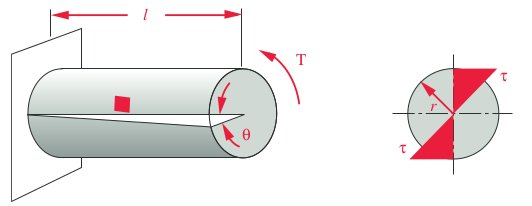
\includegraphics[width=\textwidth]{images/img501.jpg}
%	\end{center}
%	\fonte{**Norton 4ed**}
%\end{figure}
%
%\begin{equation}\label{eq:Eq_505}
%\theta = \frac{Tl}{GJ}
%\end{equation}
%
%\begin{equation}\label{eq:Eq_506}
%\tau = \frac{Tr}{J}
%\end{equation}
%
%\vspace{\baselineskip}
%
%\section{Sensoriamento de deformações}
%
%\subsection{Strain gauge}
%
%Strain gauges são sensores que sofrem alterações de resistência elétrica conforme a deformação ocorrida na superfície em que são aplicados, uma relação entre a variação de resistência e deformação em um strain gauge é denominado gauge factor.
%
%\begin{equation}\label{eq:Eq_507}
%K\varepsilon = \frac{\Delta R_{s}}{R_{s}}
%\end{equation}
%
%onde
%
%K: Gauge factor
%
%$\Delta R_{s}$: variação de resistência no strain gauge
%
%$R_{s}$: resistência nominal do strain gauge
%
%\vspace{\baselineskip}
%
%O resistor a ser utilizado é do modelo B350-3AA, que possui resistência nominal de 350 ohms e gauge factor de 2. 
%
%\subsection{Ponte de Wheatstone}
%
%Devido às pequenas variações de resistência durante o funcionamento do strain gauge, o que gera pequenas variações de tensão em seu funcionamento no circuito elétrico, é necessária sua montagem como parte de uma Ponte de Wheatstone. Esse tipo de montagem permite a instrumentação desses sensores, devido a melhor sensibilidade na leitura do voltímetro V.
%
%\begin{figure}[htb]
%	\caption{\label{fig:Fig_502}esquema basico de ponte de Wheatstone}
%	\begin{center}
%		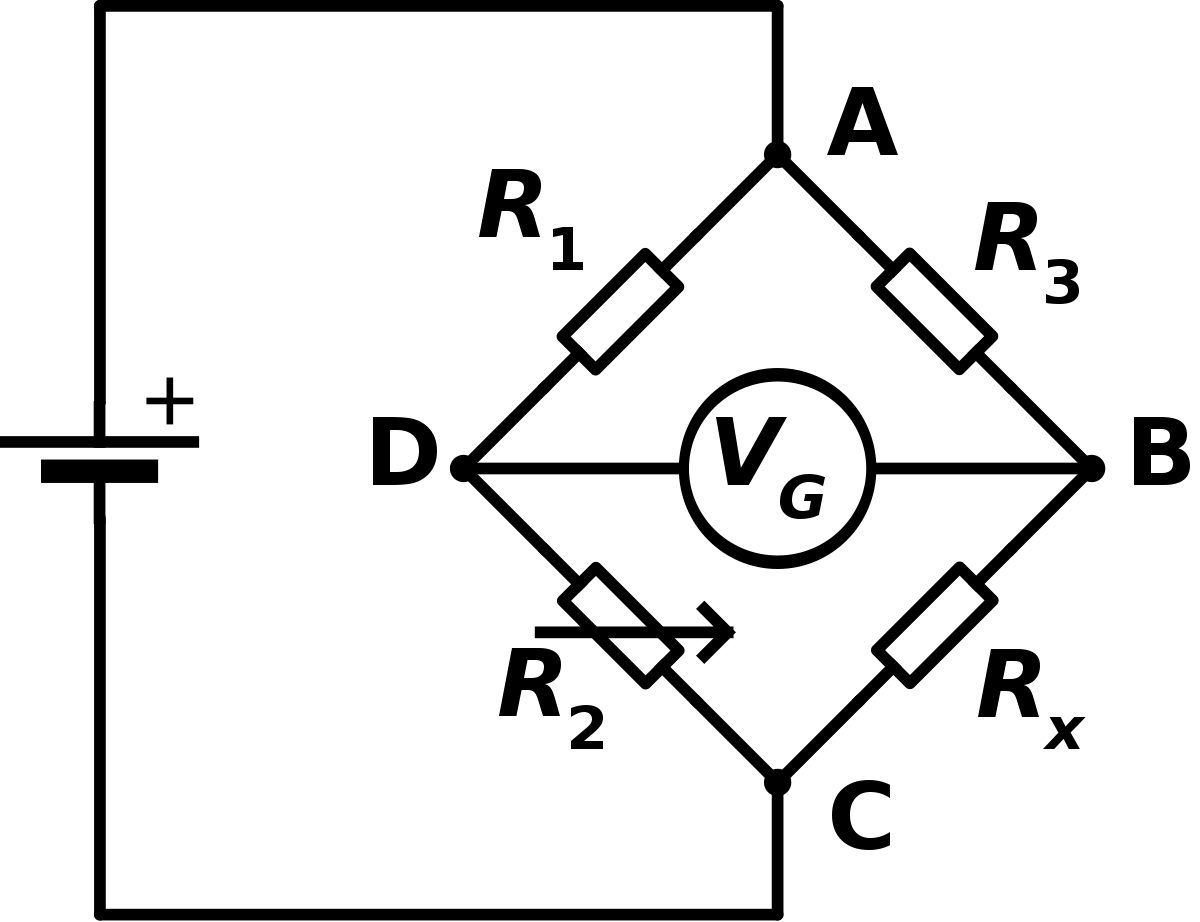
\includegraphics[width=\textwidth]{images/img502.png}
%	\end{center}
%	\fonte{*internet**}
%\end{figure}
%
%Substituindo a resistência R4 pelo strain gauge e utilizando resistores com resistências iguais ao do valor nominal do sensor em R1, R2 e R3, Utilizando as leis de Kirchoff para o circuito, a equação de transferência do circuito é encontrada.
%
%\begin{equation}\label{eq:Eq_508}
%\frac{V}{V_{in}} = \frac{K \varepsilon}{4 = K \varepsilon}
%\end{equation}
%
%onde
%
%Vin: Tensão de alimentação do circuito
%
%V: Tensão mostrada pelo voltímetro Vg



\chapter{Experimento}%\label{cap:Experimento}
%
%O presente capítulo demonstra a metodologia que será utilizada na execução do experimento e processamento dos dados obtidos.
%
%\vspace{\baselineskip}
%- Componentes necessários
%
%- Bancada Nat Geo
%
%- Comunicação Arduino PC
%
%- Pós processamento de dados
%
%- Pesquisas de metodologia de projeto
%
%- Projeto do dispositivo
%
%\section{Análise computacional}
%
%Descrever as rotinas computacionais desenvolvidas e seus resultados
%
%\vspace{\baselineskip}
%- Simulação feita no python
%
%- Resultados de torque esperados para aplicações
%
%- Verificar se os componentes são adequados
%
%\section{Microprocessador}
%
%Arduino (Documentação Arduino): “plataforma eletrônica de código aberto baseado em hardwares e softwares fáceis de usar” “as placas são capazes de ler entradas, e transformadas em saídas” “você pode dizer a sua placa o que fazer enviando um conjunto de informações ao microcontrolador na placa. Para isso, você utiliza a linguagem de programação Arduino, e o Arduino software (IDE), baseado em processamento” “Professores e estudantes utilizam para construção de instrumentos científicos de baixo custo. Designers e arquitetos constroem protótipos interativos” Vantagens: inexpensive, cross-platform, simple, clear programming environment, open source and extensible software and hardware
%
%Função analogRead(): Função que lê o valor relativo a tensão no pino de análise, sua saída varia entre 0 e 1023, o que significa 0 a 5V respectivamente (dependendo da placa pode ser 0 a 3.3V) (0.0049mV/unidade) “it takes around 100 microseconds (0.0001s) to read an analog input, so the maximum reading rate is about 10KHz”
%
%\section{Obtenção dos sinais}
%
%Análise no domínio do tempo de sistemas em tempo discreto (Lathi): “um sinal em tempo discreto é basicamente uma sequência de números. [...] podem aparecer como resultado da amostragem de sinais contínuos no tempo em sistemas amostrados de filtragem digital.”, “sistemas cujas entradas e saídas são sinais em tempo discreto são chamados de sistemas em tempo discreto ou simplesmente sistemas discretos. Um computador digital é um exemplo típico desse tipo de sistema. ”
%
%Amostragem: a ponte entre o contínuo e o discreto: “Um sinal em tempo contínuo pode ser processado, a partir de suas amostras, por um sistema que opere em tempo discreto. para isso, é importante manter a taxa de amostragem do sinal suficientemente alta para permitir a reconstrução sem erro (ou com um erro dentro de uma dada tolerância) do sinal original”, “O teorema da amostragem é a ponte entre os mundos de tempo contínuo e tempo discreto. A informação inerente em um sinal em tempo contínuo amostrado é equivalente a de um sinal em tempo discreto”
%
%Teorema da amostragem: Lathi demonstra que “um sinal em tempo real cujo espectro é limitado em faixa a B Hz pode ser reconstruído exatamente (sem qualquer erro) de suas amostras tomadas uniformemente a uma taxa de fz > 2B Hz”
%
%Conversão analógica para digital: “um sinal analógico é caracterizado pelo fato de sua amplitude poder assumir qualquer valor em um faixa contínua [...] um sinal analógico pode ser convertido em um sinal digital através de amostragem e quantização (arredondamento).”
%
%\vspace{\baselineskip}
%fig 8-14: conversão analógica pra digital (A/D)
%\vspace{\baselineskip}
%
%\section{Processamento dos dados}
%
%\section{Validação do dispositivo}
%
%-Calibração do dispositivo
%
%-Testes experimentais utilizando a bancada do nat geo
%
%*Falar sobre as ferramentas de validação estatística e seus resultados nas analises.



\phantomsection


\chapter{Resultados}%\label{cap:Resultados}


\phantomsection

\chapter{Conclusões}%\label{cap:Conclusões}


    % Finaliza a parte no bookmark do PDF para que se inicie o bookmark na raiz
    % e adiciona espaço de parte no Sumário
    \phantompart

    % Conclusão (outro exemplo de capítulo sem numeração e presente no sumário)
    
\phantomsection

\chapter{Considerações Finais}

O objetivo geral do trabalho foi considerado como alcançado, uma vez que foi desenvolvido com sucesso um protótipo funcional.
Por mais que não foi possível a sua aplicação em um eixo rotacional, o seu conceito de funcionamento foi validado por um experimento estático.

O objetivos específico de desenvolver um protótipo focado na utilização por um público alvo foi parcialmente alcançado.
As etapas e as decisões das fases da metodologia de projeto foram tomadas considerando os requisitos dos clientes, porém não foi possível validar
um dos componentes essenciais do funcionamento do dispositivo na etapa de experimentação, os testes foram realizados utilizando um módulo de conversão
de sinal diferentes do definido no projeto conceitual.

As documentações necessárias para replicar o dispositivo se encontram nos \autoref{ch:projeto-elétrico}, \autoref{ch:algoritmo-de-programação-do-controlador-do-dispositivo}
e \autoref{ch:algoritmos-desenvolvidos-para-o-software-de-conexão}.
Porém o projeto detalhado, principalmente o projeto mecânico ainda pode ser consideravelmente melhorado adicionando com maior detalhe os encaixes para os componentes de alimentação
e os encaixes dos módulos no encapsulamento do dispositivo.

Os valores obtidos pelo experimento se mostraram com erros aceitáveis para aplicações de baixo custo, principalmente quando comparados com os
valores obtidos por um dispositivo homologado, logo, a precisão do dispositivo foi considerada como aceitável para a utilização por equipes de competição,
uma vez que atualmente é observado a dificuldade pela obtenção desses tipos de dados.

Os dados obtidos pelo dispositivo ainda podem apresentar melhores valores de faixa de leitura e precisão, para isso é sugerido a implementação de um método de zerar a tensão
inicial da ponte de Wheatstone substituindo um dos resistores da ponte por elemento de resistência variável que pode ser ajustado pelo usuário, como um potenciômetro.

Também deve-se apontar que uma equipe de competição provavelmente já estará utilizando dispositivos para obtenção de dados de sensor, logo, pode-se integrar o dispositivo desenvolvido
á um dispositivo central de obtenção, caso esse suporte uma obtenção de dados utilizando comunicação via rede sem fio.

O software de obtenção de dados desenvolvido pode ser facilmente modificado e expandido para a representação de diferentes tipos de dados, logo, ele pode ser aplicado para aplicações
além de obter os dados do dispositivo desenvolvido.

O Método de obtenção de dados via rede de internet faz com que o dispositivo possa ser utilizado para aplicações remotas, como em aplicações de telemetria industrial, porém
deve-se notar as limitações em relação a precisão dos dados obtidos.

O preço final encontrado do dispositivo se mostra consideravelmente menor do que os dos dispositivos encontrados no mercado, porém, deve-se notar que os módulos utilizados são
desenvolvidos para aplicações específicas e normalmente utilizados por entusiastas em pequenos projetos, logo, não se pode confirmar a confiabilidade e precisão ao longo do tempo,
assim como a durabilidade de um dispositivo fabricado.

\subsection{Trabalhos futuros sugeridos}

Possíveis melhorias do dispositivo e expansão do estudo desenvolvido pelo autor são apresentados na listagem a seguir:

\begin{alineas}
    \item{Utilizar o dispositivo para obter os dados em uma aplicação veicular}
    \item{Estudar o efeito do desbalanceamento de massa do dispositivo no eixo em que está acoplado}
    \item{Estudar o impacto da utilização de diferentes elementos extensômetros na obtenção do sinal pelo dispositivo}
    \item{Realizar o experimento utilizando uma ponte de Wheatstone composta unicamente por extensômetros}
    \item{Realizar o experimento utilizando o dispositivo de torção desenvolvido por Minela (2017)}
    \item{Obter os valores de deformação de um eixo utilizando primariamente os valores de tensão obtidos utilizando uma função de transferência}
    \item{Estudar efeitos de atraso na transmissão dos sinais por comunicação sem fio}
    \item{Desenvolver método para transmissão de dados em longas distâncias e em locais que não possuem redes de internet sem fio disponíveis}
\end{alineas}


    % ELEMENTOS PÓS-TEXTUAIS
    \postextual
    \setlength\beforechapskip{0pt}
    \setlength\midchapskip{15pt}
    \setlength\afterchapskip{15pt}

    % Referências bibliográficas
    \begingroup
        % https://tex.stackexchange.com/questions/163559/how-to-modify-line-spacing-per-entry-of-bibliography
        % https://tex.stackexchange.com/questions/19105/how-can-i-put-more-space-between-bibliography-entries-biblatex
        \setlength\bibitemsep{\baselineskip}
        \advisor{}{\linespread{1.18}\selectfont}

        % https://tex.stackexchange.com/questions/17128/using-bibtex-to-make-a-list-of-references-without-having-citations-in-the-body
        \nocite{*}
        \printbibliography[title=\lang{REFERENCES}{REFERÊNCIAS}]
    \endgroup

    % Glossário, consulte o manual da classe abntex2 para orientações sobre o glossário.
    % \ifforcedinclude\else\glossary\fi

    % Inicia os apêndices
    \begin{apendicesenv}
        % Imprime uma página indicando o início dos apêndices
        \ifforcedinclude\else\partapendices\fi
        \setlength\beforechapskip{50pt}
        \setlength\midchapskip{20pt}
        \setlength\afterchapskip{20pt}

        \chapter{Projeto elétrico}\label{ch:projeto-elétrico}

\includepdf{aftertext/Projeto_eletrico.pdf}

%
%
%
%%
%% How to fix the Underfull \vbox badness has occurred while \output is active on my memoir chapter style?
%% https://tex.stackexchange.com/questions/387881/how-to-fix-the-underfull-vbox-badness-has-occurred-while-output-is-active-on-m
%%
%
%% ---
%
%\lang
%{\chapter[Page not filled]{Since this page is not being completely filled, it is generating the bottom bottom of the page}}
%{\chapter[Página não gerada]{Como esta página não está sendo completamente preenchida, ele está gerando a caixa inferior inferior da página}}
%% ---
%
%
%% Multiple-language document - babel - selectlanguage vs begin/end{otherlanguage}
%% https://tex.stackexchange.com/questions/36526/multiple-language-document-babel-selectlanguage-vs-begin-endotherlanguage
%\begin{otherlanguage*}{english}
%
%\showfont
%
%1. How to display the font size in use in the final output,
%2. How to display the font size in use in the final output,
%3. How to display the font size in use in the final output,
%4. How to display the font size in use in the final output,
%5. How to display the font size in use in the final output,
%6. How to display the font size in use in the final output,
%7. How to display the font size in use in the final output,
%8. How to display the font size in use in the final output,
%9. How to display the font size in use in the final output,
%
%
%% As this page is not being completely filled, it is generating the page bottom bad box.
%% Fix Underfull \vbox (badness 10000) has occurred while \output is active
%%
%% \flushbottom vs \raggedbottom
%% https://tex.stackexchange.com/questions/65355/flushbottom-vs-raggedbottom
%\newpage
%
%
%
%\section[Some encoding tests]{\showfont}
%
%1. How to display the font size in use in the final output,
%2. How to display the font size in use in the final output,
%3. How to display the font size in use in the final output,
%4. How to display the font size in use in the final output,
%5. How to display the font size in use in the final output,
%6. How to display the font size in use in the final output,
%
%7. How to display the font size in use in the final output,
%8. How to display the font size in use in the final output,
%9. How to display the font size in use in the final output,
%10. How to display the font size in use in the final output,
%11. How to display the font size in use in the final output,
%12. How to display the font size in use in the final output,
%
%\subsection{\showfont}
%
%1. How to display the font size in use in the final output,
%2. How to display the font size in use in the final output,
%3. How to display the font size in use in the final output,
%4. How to display the font size in use in the final output,
%5. How to display the font size in use in the final output,
%6. How to display the font size in use in the final output,
%
%7. How to display the font size in use in the final output,
%8. How to display the font size in use in the final output,
%9. How to display the font size in use in the final output,
%10. How to display the font size in use in the final output,
%11. How to display the font size in use in the final output,
%12. How to display the font size in use in the final output,
%
%\subsubsection{\showfont}
%
%1. How to display the font size in use in the final output,
%2. How to display the font size in use in the final output,
%3. How to display the font size in use in the final output,
%4. How to display the font size in use in the final output,
%5. How to display the font size in use in the final output,
%6. How to display the font size in use in the final output,
%
%7. How to display the font size in use in the final output,
%8. How to display the font size in use in the final output,
%9. How to display the font size in use in the final output,
%10. How to display the font size in use in the final output,
%11. How to display the font size in use in the final output,
%12. How to display the font size in use in the final output,
%
%\subsubsubsection{\showfont}
%
%1. How to display the font size in use in the final output,
%2. How to display the font size in use in the final output,
%3. How to display the font size in use in the final output,
%4. How to display the font size in use in the final output,
%5. How to display the font size in use in the final output,
%6. How to display the font size in use in the final output,
%7. How to display the font size in use in the final output,
%
%8. How to display the font size in use in the final output,
%9. How to display the font size in use in the final output,
%10. How to display the font size in use in the final output,
%11. How to display the font size in use in the final output,
%12. How to display the font size in use in the final output,
%
%
%Lipsum me [31-35]
%
%\end{otherlanguage*}
%
%

    \end{apendicesenv}

    % Inicia os anexos
    \begin{anexosenv}
        % Imprime uma página indicando o início dos anexos
        \ifforcedinclude\else\partanexos\fi
        \setlength\beforechapskip{50pt}
        \setlength\midchapskip{20pt}
        \setlength\afterchapskip{20pt}

        

%
% How to fix the Underfull \vbox badness has occurred while \output is active on my memoir chapter style?
% https://tex.stackexchange.com/questions/387881/how-to-fix-the-underfull-vbox-badness-has-occurred-while-output-is-active-on-m
%

% ----------------------------------------------------------
\chapter{\lang{Article published in SOBRAEP magazine}{Artigo publicado}}
% ----------------------------------------------------------


% Multiple-language document - babel - selectlanguage vs begin/end{otherlanguage}
% https://tex.stackexchange.com/questions/36526/multiple-language-document-babel-selectlanguage-vs-begin-endotherlanguage
\begin{otherlanguage*}{english}

% An environment for setting \emergencystretch locally
% https://tex.stackexchange.com/questions/84510/an-environment-for-setting-emergencystretch-locally
{
    \setlength{\emergencystretch}{10pt}
    \section[English guidelines for publication]
    {English guidelines for publication - TITLE HERE (14 PT TYPE SIZE, UPPERCASE, BOLD, CENTERED)}
}
    \noindent\textbf{Abstract:}
    The objective of this document is to instruct the authors about the preparation of the
    manuscript for its submission to the Revista Eletrônica de Potência (Brazilian Power Electronics
    Journal).~The authors should use these guidelines for preparing both the initial and final
    versions of their paper. Additional information about procedures and guidelines for publication
    can be obtained directly with the editor, or through the web site
    \url{http://www.sobraep.org.br/revista}. This text was written according to these guidelines

\end{otherlanguage*}

% What is a “Overfull \hbox (9.89561pt too wide)”?
% https://tex.stackexchange.com/questions/111948/what-is-a-overfull-hbox-9-89561pt-too-wide
interwordspace: \the\fontdimen2\font

interwordstretch: \the\fontdimen3\font

emergencystretch: \the\emergencystretch\par\relax


\modifiedincludepdf{-}{ArtigoSOBRAEP}{pictures/SOBRAEP.pdf}{0.9}



        


%
% How to fix the Underfull \vbox badness has occurred while \output is active on my memoir chapter style?
% https://tex.stackexchange.com/questions/387881/how-to-fix-the-underfull-vbox-badness-has-occurred-while-output-is-active-on-m
%

% ----------------------------------------------------------
\lang
{\chapter[Sample example]{How to display the font size in use in the final output}}
{\chapter[Anexo exemplo]{Como exibir o tamanho da fonte em uso na saída final}}
% ----------------------------------------------------------


% Multiple-language document - babel - selectlanguage vs begin/end{otherlanguage}
% https://tex.stackexchange.com/questions/36526/multiple-language-document-babel-selectlanguage-vs-begin-endotherlanguage
\begin{otherlanguage*}{english}

\showfont

1. How to display the font size in use in the final output,
2. How to display the font size in use in the final output,
3. How to display the font size in use in the final output,


\section[Some encoding tests]{\showfont}

1. How to display the font size in use in the final output,
2. How to display the font size in use in the final output,
3. How to display the font size in use in the final output,
4. How to display the font size in use in the final output,
5. How to display the font size in use in the final output,
6. How to display the font size in use in the final output,

7. How to display the font size in use in the final output,
8. How to display the font size in use in the final output,
9. How to display the font size in use in the final output,
10. How to display the font size in use in the final output,
11. How to display the font size in use in the final output,
12. How to display the font size in use in the final output,

\subsection{\showfont}

1. How to display the font size in use in the final output,
2. How to display the font size in use in the final output,
3. How to display the font size in use in the final output,
4. How to display the font size in use in the final output,
5. How to display the font size in use in the final output,
6. How to display the font size in use in the final output,

7. How to display the font size in use in the final output,
8. How to display the font size in use in the final output,
9. How to display the font size in use in the final output,
10. How to display the font size in use in the final output,
11. How to display the font size in use in the final output,
12. How to display the font size in use in the final output,

\subsubsection{\showfont}

1. How to display the font size in use in the final output,
2. How to display the font size in use in the final output,
3. How to display the font size in use in the final output,
4. How to display the font size in use in the final output,
5. How to display the font size in use in the final output,
6. How to display the font size in use in the final output,

7. How to display the font size in use in the final output,
8. How to display the font size in use in the final output,
9. How to display the font size in use in the final output,
10. How to display the font size in use in the final output,
11. How to display the font size in use in the final output,
12. How to display the font size in use in the final output,

\subsubsubsection{\showfont}

1. How to display the font size in use in the final output,
2. How to display the font size in use in the final output,
3. How to display the font size in use in the final output,
4. How to display the font size in use in the final output,
5. How to display the font size in use in the final output,
6. How to display the font size in use in the final output,
7. How to display the font size in use in the final output,

8. How to display the font size in use in the final output,
9. How to display the font size in use in the final output,
10. How to display the font size in use in the final output,
11. How to display the font size in use in the final output,
12. How to display the font size in use in the final output,


Lipsum me [55-65]

\end{otherlanguage*}



    \end{anexosenv}

    % INDICE REMISSIVO
    \ifforcedinclude\else
        \phantompart
        \printindex
    \fi

\end{document}

